\chapter{Simulations}
\label{C:simulations}
This chapter is a computational companion to chapter~\ref{C:stein-proof}.  

\section{Preliminaries}
First, we provide simulations accompanying section~\ref{S:stein-proof-preliminaries}.  We generate 
i.i.d. samples $\{u_i\}_{i=1}^{N} \sim \Normal(-1, 1)$ and $\{u_i\}_{i=N+1}^{2N} \sim \Normal(1, 1)$
for exponentially spaced values of $N \in \{\text{floor}(10^{.5+.5i})\}_{i=1}^7$.  The $u_i$ are scaled
and centered, and for each $N$, we perform $10,000$ permutations.  

We plot Monte Carlo estimates of the means of each term, scaled by the rate of our bound, along with
95\%ile bootstrap confidence intervals for different values of $p \in \{2, 4, 6, 8\}$.

\begin{figure}[!ht]
  \centering
  % Created by tikzDevice version 0.6.2 on 2012-04-22 09:19:32
% !TEX encoding = UTF-8 Unicode
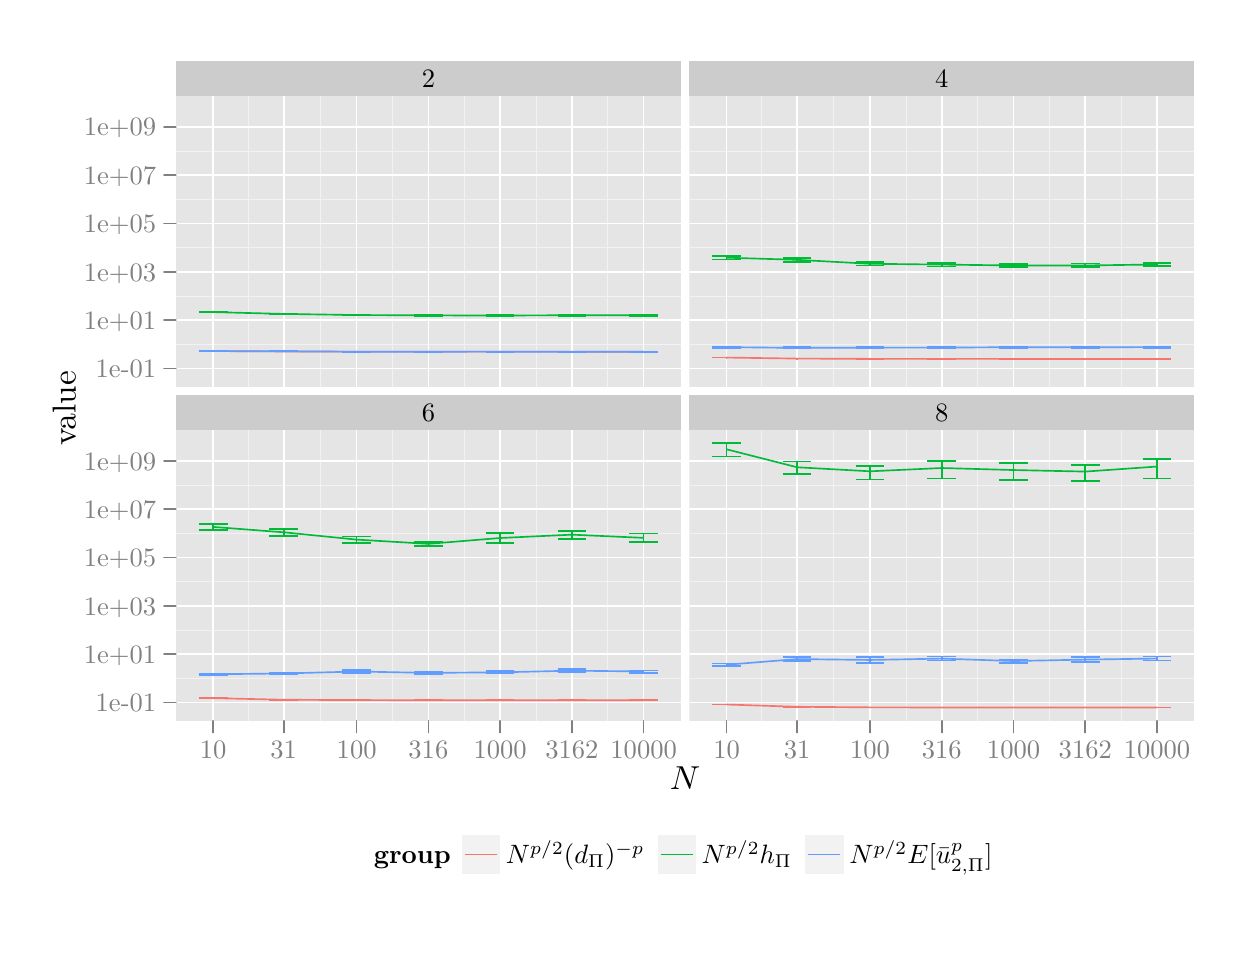
\begin{tikzpicture}[x=1pt,y=1pt]
\definecolor[named]{drawColor}{rgb}{0.00,0.00,0.00}
\definecolor[named]{fillColor}{rgb}{1.00,1.00,1.00}
\fill[color=fillColor,fill opacity=0.00,] (0,0) rectangle (433.62,325.21);
\begin{scope}
\path[clip] (  0.00,  0.00) rectangle (433.62,325.21);
\definecolor[named]{drawColor}{rgb}{0.41,0.16,0.58}
\end{scope}
\begin{scope}
\path[clip] (  0.00,  0.00) rectangle (433.62,325.21);
\definecolor[named]{drawColor}{rgb}{0.41,0.16,0.58}
\end{scope}
\begin{scope}
\path[clip] (  0.00,  0.00) rectangle (433.62,325.21);
\definecolor[named]{drawColor}{rgb}{0.41,0.16,0.58}
\end{scope}
\begin{scope}
\path[clip] (  0.00,  0.00) rectangle (433.62,325.21);
\definecolor[named]{drawColor}{rgb}{0.41,0.16,0.58}
\end{scope}
\begin{scope}
\path[clip] (  0.00,  0.00) rectangle (433.62,325.21);
\definecolor[named]{drawColor}{rgb}{0.41,0.16,0.58}
\end{scope}
\begin{scope}
\path[clip] (  0.00,  0.00) rectangle (433.62,325.21);
\definecolor[named]{drawColor}{rgb}{0.41,0.16,0.58}
\end{scope}
\begin{scope}
\path[clip] (  0.00,  0.00) rectangle (433.62,325.21);
\definecolor[named]{drawColor}{rgb}{0.41,0.16,0.58}
\end{scope}
\begin{scope}
\path[clip] (  0.00,  0.00) rectangle (433.62,325.21);
\definecolor[named]{drawColor}{rgb}{0.41,0.16,0.58}
\end{scope}
\begin{scope}
\path[clip] ( 53.55,195.47) rectangle (236.06,300.54);
\definecolor[named]{drawColor}{rgb}{0.41,0.16,0.58}
\end{scope}
\begin{scope}
\path[clip] (  0.00,  0.00) rectangle (433.62,325.21);
\definecolor[named]{drawColor}{rgb}{0.41,0.16,0.58}
\end{scope}
\begin{scope}
\path[clip] (239.07,195.47) rectangle (421.58,300.54);
\definecolor[named]{drawColor}{rgb}{0.41,0.16,0.58}
\end{scope}
\begin{scope}
\path[clip] (  0.00,  0.00) rectangle (433.62,325.21);
\definecolor[named]{drawColor}{rgb}{0.41,0.16,0.58}
\end{scope}
\begin{scope}
\path[clip] ( 53.55, 74.76) rectangle (236.06,179.83);
\definecolor[named]{drawColor}{rgb}{0.41,0.16,0.58}
\end{scope}
\begin{scope}
\path[clip] (  0.00,  0.00) rectangle (433.62,325.21);
\definecolor[named]{drawColor}{rgb}{0.41,0.16,0.58}
\end{scope}
\begin{scope}
\path[clip] (239.07, 74.76) rectangle (421.58,179.83);
\definecolor[named]{drawColor}{rgb}{0.41,0.16,0.58}
\end{scope}
\begin{scope}
\path[clip] (  0.00,  0.00) rectangle (433.62,325.21);
\definecolor[named]{drawColor}{rgb}{0.41,0.16,0.58}
\end{scope}
\begin{scope}
\path[clip] (  0.00,  0.00) rectangle (433.62,325.21);
\definecolor[named]{drawColor}{rgb}{0.41,0.16,0.58}
\end{scope}
\begin{scope}
\path[clip] (  0.00,  0.00) rectangle (433.62,325.21);
\definecolor[named]{drawColor}{rgb}{0.41,0.16,0.58}
\end{scope}
\begin{scope}
\path[clip] (  0.00,  0.00) rectangle (433.62,325.21);
\definecolor[named]{drawColor}{rgb}{0.41,0.16,0.58}
\end{scope}
\begin{scope}
\path[clip] (  0.00,  0.00) rectangle (433.62,325.21);
\definecolor[named]{drawColor}{rgb}{0.41,0.16,0.58}
\end{scope}
\begin{scope}
\path[clip] (  0.00,  0.00) rectangle (433.62,325.21);
\definecolor[named]{drawColor}{rgb}{0.41,0.16,0.58}
\end{scope}
\begin{scope}
\path[clip] (  0.00,  0.00) rectangle (433.62,325.21);
\definecolor[named]{drawColor}{rgb}{0.41,0.16,0.58}
\end{scope}
\begin{scope}
\path[clip] (  0.00,  0.00) rectangle (433.62,325.21);
\definecolor[named]{drawColor}{rgb}{0.41,0.16,0.58}
\end{scope}
\begin{scope}
\path[clip] (  0.00,  0.00) rectangle (433.62,325.21);
\definecolor[named]{drawColor}{rgb}{0.41,0.16,0.58}
\end{scope}
\begin{scope}
\path[clip] (  0.00,  0.00) rectangle (433.62,325.21);
\definecolor[named]{drawColor}{rgb}{0.41,0.16,0.58}
\end{scope}
\begin{scope}
\path[clip] (  0.00,  0.00) rectangle (433.62,325.21);
\definecolor[named]{drawColor}{rgb}{0.41,0.16,0.58}
\end{scope}
\begin{scope}
\path[clip] (  0.00,  0.00) rectangle (433.62,325.21);
\definecolor[named]{drawColor}{rgb}{0.41,0.16,0.58}
\end{scope}
\begin{scope}
\path[clip] (  0.00,  0.00) rectangle (433.62,325.21);
\definecolor[named]{drawColor}{rgb}{0.41,0.16,0.58}
\end{scope}
\begin{scope}
\path[clip] (  0.00,  0.00) rectangle (433.62,325.21);
\definecolor[named]{drawColor}{rgb}{0.41,0.16,0.58}
\end{scope}
\begin{scope}
\path[clip] (  0.00,  0.00) rectangle (433.62,325.21);
\definecolor[named]{drawColor}{rgb}{0.41,0.16,0.58}
\end{scope}
\begin{scope}
\path[clip] (  0.00,  0.00) rectangle (433.62,325.21);
\definecolor[named]{drawColor}{rgb}{0.41,0.16,0.58}
\end{scope}
\begin{scope}
\path[clip] (  0.00,  0.00) rectangle (433.62,325.21);
\definecolor[named]{drawColor}{rgb}{0.41,0.16,0.58}
\end{scope}
\begin{scope}
\path[clip] (  0.00,  0.00) rectangle (433.62,325.21);
\definecolor[named]{drawColor}{rgb}{0.41,0.16,0.58}
\end{scope}
\begin{scope}
\path[clip] (  0.00,  0.00) rectangle (433.62,325.21);
\definecolor[named]{drawColor}{rgb}{0.41,0.16,0.58}
\end{scope}
\begin{scope}
\path[clip] (  0.00,  0.00) rectangle (433.62,325.21);
\definecolor[named]{drawColor}{rgb}{0.41,0.16,0.58}
\end{scope}
\begin{scope}
\path[clip] (  0.00,  0.00) rectangle (433.62,325.21);
\definecolor[named]{drawColor}{rgb}{0.41,0.16,0.58}
\end{scope}
\begin{scope}
\path[clip] (  0.00,  0.00) rectangle (433.62,325.21);
\definecolor[named]{drawColor}{rgb}{0.41,0.16,0.58}
\end{scope}
\begin{scope}
\path[clip] (  0.00,  0.00) rectangle (433.62,325.21);
\definecolor[named]{drawColor}{rgb}{0.41,0.16,0.58}
\end{scope}
\begin{scope}
\path[clip] (  0.00,  0.00) rectangle (433.62,325.21);
\definecolor[named]{drawColor}{rgb}{0.41,0.16,0.58}
\end{scope}
\begin{scope}
\path[clip] (  0.00,  0.00) rectangle (433.62,325.21);
\definecolor[named]{drawColor}{rgb}{0.41,0.16,0.58}
\end{scope}
\begin{scope}
\path[clip] (  0.00,  0.00) rectangle (433.62,325.21);
\definecolor[named]{drawColor}{rgb}{0.41,0.16,0.58}
\end{scope}
\begin{scope}
\path[clip] (  0.00,  0.00) rectangle (433.62,325.21);
\definecolor[named]{drawColor}{rgb}{0.41,0.16,0.58}
\end{scope}
\begin{scope}
\path[clip] (  0.00,  0.00) rectangle (433.62,325.21);
\definecolor[named]{drawColor}{rgb}{0.41,0.16,0.58}
\end{scope}
\begin{scope}
\path[clip] (  0.00,  0.00) rectangle (433.62,325.21);
\definecolor[named]{drawColor}{rgb}{0.41,0.16,0.58}
\end{scope}
\begin{scope}
\path[clip] (  0.00,  0.00) rectangle (433.62,325.21);
\definecolor[named]{drawColor}{rgb}{0.41,0.16,0.58}
\end{scope}
\begin{scope}
\path[clip] (  0.00,  0.00) rectangle (433.62,325.21);
\definecolor[named]{drawColor}{rgb}{0.41,0.16,0.58}
\end{scope}
\begin{scope}
\path[clip] (  0.00,  0.00) rectangle (433.62,325.21);
\definecolor[named]{drawColor}{rgb}{0.41,0.16,0.58}
\end{scope}
\begin{scope}
\path[clip] (  0.00,  0.00) rectangle (433.62,325.21);
\definecolor[named]{drawColor}{rgb}{0.41,0.16,0.58}
\end{scope}
\begin{scope}
\path[clip] (  0.00,  0.00) rectangle (433.62,325.21);
\definecolor[named]{drawColor}{rgb}{0.41,0.16,0.58}
\definecolor[named]{fillColor}{rgb}{1.00,1.00,1.00}

\draw[fill=fillColor,draw opacity=0.00,] (  0.00,  0.00) rectangle (433.62,325.21);
\end{scope}
\begin{scope}
\path[clip] (  0.00,  0.00) rectangle (433.62,325.21);
\definecolor[named]{drawColor}{rgb}{0.41,0.16,0.58}
\end{scope}
\begin{scope}
\path[clip] ( 53.55,195.47) rectangle (236.06,300.54);
\definecolor[named]{drawColor}{rgb}{0.41,0.16,0.58}
\definecolor[named]{fillColor}{rgb}{0.90,0.90,0.90}

\draw[fill=fillColor,draw opacity=0.00,] ( 53.55,195.47) rectangle (236.06,300.54);
\definecolor[named]{drawColor}{rgb}{0.95,0.95,0.95}

\draw[color=drawColor,line width= 0.3pt,line cap=round,line join=round,fill opacity=0.00,] ( 53.55,210.76) --
	(236.06,210.76);

\draw[color=drawColor,line width= 0.3pt,line cap=round,line join=round,fill opacity=0.00,] ( 53.55,228.23) --
	(236.06,228.23);

\draw[color=drawColor,line width= 0.3pt,line cap=round,line join=round,fill opacity=0.00,] ( 53.55,245.70) --
	(236.06,245.70);

\draw[color=drawColor,line width= 0.3pt,line cap=round,line join=round,fill opacity=0.00,] ( 53.55,263.17) --
	(236.06,263.17);

\draw[color=drawColor,line width= 0.3pt,line cap=round,line join=round,fill opacity=0.00,] ( 53.55,280.64) --
	(236.06,280.64);

\draw[color=drawColor,line width= 0.3pt,line cap=round,line join=round,fill opacity=0.00,] ( 79.77,195.47) --
	( 79.77,300.54);

\draw[color=drawColor,line width= 0.3pt,line cap=round,line join=round,fill opacity=0.00,] (105.69,195.47) --
	(105.69,300.54);

\draw[color=drawColor,line width= 0.3pt,line cap=round,line join=round,fill opacity=0.00,] (131.83,195.47) --
	(131.83,300.54);

\draw[color=drawColor,line width= 0.3pt,line cap=round,line join=round,fill opacity=0.00,] (157.76,195.47) --
	(157.76,300.54);

\draw[color=drawColor,line width= 0.3pt,line cap=round,line join=round,fill opacity=0.00,] (183.69,195.47) --
	(183.69,300.54);

\draw[color=drawColor,line width= 0.3pt,line cap=round,line join=round,fill opacity=0.00,] (209.61,195.47) --
	(209.61,300.54);
\definecolor[named]{drawColor}{rgb}{1.00,1.00,1.00}

\draw[color=drawColor,line width= 0.6pt,line cap=round,line join=round,fill opacity=0.00,] ( 53.55,202.03) --
	(236.06,202.03);

\draw[color=drawColor,line width= 0.6pt,line cap=round,line join=round,fill opacity=0.00,] ( 53.55,219.50) --
	(236.06,219.50);

\draw[color=drawColor,line width= 0.6pt,line cap=round,line join=round,fill opacity=0.00,] ( 53.55,236.97) --
	(236.06,236.97);

\draw[color=drawColor,line width= 0.6pt,line cap=round,line join=round,fill opacity=0.00,] ( 53.55,254.44) --
	(236.06,254.44);

\draw[color=drawColor,line width= 0.6pt,line cap=round,line join=round,fill opacity=0.00,] ( 53.55,271.91) --
	(236.06,271.91);

\draw[color=drawColor,line width= 0.6pt,line cap=round,line join=round,fill opacity=0.00,] ( 53.55,289.38) --
	(236.06,289.38);

\draw[color=drawColor,line width= 0.6pt,line cap=round,line join=round,fill opacity=0.00,] ( 67.03,195.47) --
	( 67.03,300.54);

\draw[color=drawColor,line width= 0.6pt,line cap=round,line join=round,fill opacity=0.00,] ( 92.51,195.47) --
	( 92.51,300.54);

\draw[color=drawColor,line width= 0.6pt,line cap=round,line join=round,fill opacity=0.00,] (118.88,195.47) --
	(118.88,300.54);

\draw[color=drawColor,line width= 0.6pt,line cap=round,line join=round,fill opacity=0.00,] (144.79,195.47) --
	(144.79,300.54);

\draw[color=drawColor,line width= 0.6pt,line cap=round,line join=round,fill opacity=0.00,] (170.73,195.47) --
	(170.73,300.54);

\draw[color=drawColor,line width= 0.6pt,line cap=round,line join=round,fill opacity=0.00,] (196.65,195.47) --
	(196.65,300.54);

\draw[color=drawColor,line width= 0.6pt,line cap=round,line join=round,fill opacity=0.00,] (222.58,195.47) --
	(222.58,300.54);
\definecolor[named]{drawColor}{rgb}{0.97,0.46,0.43}

\draw[color=drawColor,line width= 0.6pt,line join=round,fill opacity=0.00,] ( 67.03,208.37) --
	( 92.51,208.20) --
	(118.88,208.15) --
	(144.79,208.14) --
	(170.73,208.14) --
	(196.65,208.13) --
	(222.58,208.13);
\definecolor[named]{drawColor}{rgb}{0.00,0.73,0.22}

\draw[color=drawColor,line width= 0.6pt,line join=round,fill opacity=0.00,] ( 67.03,222.43) --
	( 92.51,221.77) --
	(118.88,221.37) --
	(144.79,221.25) --
	(170.73,221.19) --
	(196.65,221.30) --
	(222.58,221.31);
\definecolor[named]{drawColor}{rgb}{0.38,0.61,1.00}

\draw[color=drawColor,line width= 0.6pt,line join=round,fill opacity=0.00,] ( 67.03,208.33) --
	( 92.51,208.25) --
	(118.88,208.12) --
	(144.79,208.12) --
	(170.73,208.14) --
	(196.65,208.07) --
	(222.58,208.14);
\definecolor[named]{drawColor}{rgb}{0.97,0.46,0.43}

\draw[color=drawColor,line width= 0.6pt,line join=round,fill opacity=0.00,] ( 61.85,208.37) --
	( 72.22,208.37);

\draw[color=drawColor,line width= 0.6pt,line join=round,fill opacity=0.00,] ( 67.03,208.37) --
	( 67.03,208.36);

\draw[color=drawColor,line width= 0.6pt,line join=round,fill opacity=0.00,] ( 61.85,208.36) --
	( 72.22,208.36);

\draw[color=drawColor,line width= 0.6pt,line join=round,fill opacity=0.00,] ( 87.32,208.20) --
	( 97.69,208.20);

\draw[color=drawColor,line width= 0.6pt,line join=round,fill opacity=0.00,] ( 92.51,208.20) --
	( 92.51,208.20);

\draw[color=drawColor,line width= 0.6pt,line join=round,fill opacity=0.00,] ( 87.32,208.20) --
	( 97.69,208.20);

\draw[color=drawColor,line width= 0.6pt,line join=round,fill opacity=0.00,] (113.69,208.15) --
	(124.06,208.15);

\draw[color=drawColor,line width= 0.6pt,line join=round,fill opacity=0.00,] (118.88,208.15) --
	(118.88,208.15);

\draw[color=drawColor,line width= 0.6pt,line join=round,fill opacity=0.00,] (113.69,208.15) --
	(124.06,208.15);

\draw[color=drawColor,line width= 0.6pt,line join=round,fill opacity=0.00,] (139.60,208.14) --
	(149.97,208.14);

\draw[color=drawColor,line width= 0.6pt,line join=round,fill opacity=0.00,] (144.79,208.14) --
	(144.79,208.14);

\draw[color=drawColor,line width= 0.6pt,line join=round,fill opacity=0.00,] (139.60,208.14) --
	(149.97,208.14);

\draw[color=drawColor,line width= 0.6pt,line join=round,fill opacity=0.00,] (165.54,208.14) --
	(175.91,208.14);

\draw[color=drawColor,line width= 0.6pt,line join=round,fill opacity=0.00,] (170.73,208.14) --
	(170.73,208.14);

\draw[color=drawColor,line width= 0.6pt,line join=round,fill opacity=0.00,] (165.54,208.14) --
	(175.91,208.14);

\draw[color=drawColor,line width= 0.6pt,line join=round,fill opacity=0.00,] (191.47,208.13) --
	(201.83,208.13);

\draw[color=drawColor,line width= 0.6pt,line join=round,fill opacity=0.00,] (196.65,208.13) --
	(196.65,208.13);

\draw[color=drawColor,line width= 0.6pt,line join=round,fill opacity=0.00,] (191.47,208.13) --
	(201.83,208.13);

\draw[color=drawColor,line width= 0.6pt,line join=round,fill opacity=0.00,] (217.39,208.13) --
	(227.76,208.13);

\draw[color=drawColor,line width= 0.6pt,line join=round,fill opacity=0.00,] (222.58,208.13) --
	(222.58,208.13);

\draw[color=drawColor,line width= 0.6pt,line join=round,fill opacity=0.00,] (217.39,208.13) --
	(227.76,208.13);
\definecolor[named]{drawColor}{rgb}{0.00,0.73,0.22}

\draw[color=drawColor,line width= 0.6pt,line join=round,fill opacity=0.00,] ( 61.85,222.60) --
	( 72.22,222.60);

\draw[color=drawColor,line width= 0.6pt,line join=round,fill opacity=0.00,] ( 67.03,222.60) --
	( 67.03,222.24);

\draw[color=drawColor,line width= 0.6pt,line join=round,fill opacity=0.00,] ( 61.85,222.24) --
	( 72.22,222.24);

\draw[color=drawColor,line width= 0.6pt,line join=round,fill opacity=0.00,] ( 87.32,221.97) --
	( 97.69,221.97);

\draw[color=drawColor,line width= 0.6pt,line join=round,fill opacity=0.00,] ( 92.51,221.97) --
	( 92.51,221.57);

\draw[color=drawColor,line width= 0.6pt,line join=round,fill opacity=0.00,] ( 87.32,221.57) --
	( 97.69,221.57);

\draw[color=drawColor,line width= 0.6pt,line join=round,fill opacity=0.00,] (113.69,221.57) --
	(124.06,221.57);

\draw[color=drawColor,line width= 0.6pt,line join=round,fill opacity=0.00,] (118.88,221.57) --
	(118.88,221.17);

\draw[color=drawColor,line width= 0.6pt,line join=round,fill opacity=0.00,] (113.69,221.17) --
	(124.06,221.17);

\draw[color=drawColor,line width= 0.6pt,line join=round,fill opacity=0.00,] (139.60,221.44) --
	(149.97,221.44);

\draw[color=drawColor,line width= 0.6pt,line join=round,fill opacity=0.00,] (144.79,221.44) --
	(144.79,221.05);

\draw[color=drawColor,line width= 0.6pt,line join=round,fill opacity=0.00,] (139.60,221.05) --
	(149.97,221.05);

\draw[color=drawColor,line width= 0.6pt,line join=round,fill opacity=0.00,] (165.54,221.38) --
	(175.91,221.38);

\draw[color=drawColor,line width= 0.6pt,line join=round,fill opacity=0.00,] (170.73,221.38) --
	(170.73,220.99);

\draw[color=drawColor,line width= 0.6pt,line join=round,fill opacity=0.00,] (165.54,220.99) --
	(175.91,220.99);

\draw[color=drawColor,line width= 0.6pt,line join=round,fill opacity=0.00,] (191.47,221.51) --
	(201.83,221.51);

\draw[color=drawColor,line width= 0.6pt,line join=round,fill opacity=0.00,] (196.65,221.51) --
	(196.65,221.12);

\draw[color=drawColor,line width= 0.6pt,line join=round,fill opacity=0.00,] (191.47,221.12) --
	(201.83,221.12);

\draw[color=drawColor,line width= 0.6pt,line join=round,fill opacity=0.00,] (217.39,221.51) --
	(227.76,221.51);

\draw[color=drawColor,line width= 0.6pt,line join=round,fill opacity=0.00,] (222.58,221.51) --
	(222.58,221.12);

\draw[color=drawColor,line width= 0.6pt,line join=round,fill opacity=0.00,] (217.39,221.12) --
	(227.76,221.12);
\definecolor[named]{drawColor}{rgb}{0.38,0.61,1.00}

\draw[color=drawColor,line width= 0.6pt,line join=round,fill opacity=0.00,] ( 61.85,208.43) --
	( 72.22,208.43);

\draw[color=drawColor,line width= 0.6pt,line join=round,fill opacity=0.00,] ( 67.03,208.43) --
	( 67.03,208.24);

\draw[color=drawColor,line width= 0.6pt,line join=round,fill opacity=0.00,] ( 61.85,208.24) --
	( 72.22,208.24);

\draw[color=drawColor,line width= 0.6pt,line join=round,fill opacity=0.00,] ( 87.32,208.36) --
	( 97.69,208.36);

\draw[color=drawColor,line width= 0.6pt,line join=round,fill opacity=0.00,] ( 92.51,208.36) --
	( 92.51,208.16);

\draw[color=drawColor,line width= 0.6pt,line join=round,fill opacity=0.00,] ( 87.32,208.16) --
	( 97.69,208.16);

\draw[color=drawColor,line width= 0.6pt,line join=round,fill opacity=0.00,] (113.69,208.22) --
	(124.06,208.22);

\draw[color=drawColor,line width= 0.6pt,line join=round,fill opacity=0.00,] (118.88,208.22) --
	(118.88,208.01);

\draw[color=drawColor,line width= 0.6pt,line join=round,fill opacity=0.00,] (113.69,208.01) --
	(124.06,208.01);

\draw[color=drawColor,line width= 0.6pt,line join=round,fill opacity=0.00,] (139.60,208.23) --
	(149.97,208.23);

\draw[color=drawColor,line width= 0.6pt,line join=round,fill opacity=0.00,] (144.79,208.23) --
	(144.79,208.01);

\draw[color=drawColor,line width= 0.6pt,line join=round,fill opacity=0.00,] (139.60,208.01) --
	(149.97,208.01);

\draw[color=drawColor,line width= 0.6pt,line join=round,fill opacity=0.00,] (165.54,208.25) --
	(175.91,208.25);

\draw[color=drawColor,line width= 0.6pt,line join=round,fill opacity=0.00,] (170.73,208.25) --
	(170.73,208.04);

\draw[color=drawColor,line width= 0.6pt,line join=round,fill opacity=0.00,] (165.54,208.04) --
	(175.91,208.04);

\draw[color=drawColor,line width= 0.6pt,line join=round,fill opacity=0.00,] (191.47,208.17) --
	(201.83,208.17);

\draw[color=drawColor,line width= 0.6pt,line join=round,fill opacity=0.00,] (196.65,208.17) --
	(196.65,207.97);

\draw[color=drawColor,line width= 0.6pt,line join=round,fill opacity=0.00,] (191.47,207.97) --
	(201.83,207.97);

\draw[color=drawColor,line width= 0.6pt,line join=round,fill opacity=0.00,] (217.39,208.25) --
	(227.76,208.25);

\draw[color=drawColor,line width= 0.6pt,line join=round,fill opacity=0.00,] (222.58,208.25) --
	(222.58,208.03);

\draw[color=drawColor,line width= 0.6pt,line join=round,fill opacity=0.00,] (217.39,208.03) --
	(227.76,208.03);
\end{scope}
\begin{scope}
\path[clip] (  0.00,  0.00) rectangle (433.62,325.21);
\definecolor[named]{drawColor}{rgb}{0.41,0.16,0.58}
\end{scope}
\begin{scope}
\path[clip] (239.07,195.47) rectangle (421.58,300.54);
\definecolor[named]{drawColor}{rgb}{0.41,0.16,0.58}
\definecolor[named]{fillColor}{rgb}{0.90,0.90,0.90}

\draw[fill=fillColor,draw opacity=0.00,] (239.07,195.47) rectangle (421.57,300.54);
\definecolor[named]{drawColor}{rgb}{0.95,0.95,0.95}

\draw[color=drawColor,line width= 0.3pt,line cap=round,line join=round,fill opacity=0.00,] (239.07,210.76) --
	(421.58,210.76);

\draw[color=drawColor,line width= 0.3pt,line cap=round,line join=round,fill opacity=0.00,] (239.07,228.23) --
	(421.58,228.23);

\draw[color=drawColor,line width= 0.3pt,line cap=round,line join=round,fill opacity=0.00,] (239.07,245.70) --
	(421.58,245.70);

\draw[color=drawColor,line width= 0.3pt,line cap=round,line join=round,fill opacity=0.00,] (239.07,263.17) --
	(421.58,263.17);

\draw[color=drawColor,line width= 0.3pt,line cap=round,line join=round,fill opacity=0.00,] (239.07,280.64) --
	(421.58,280.64);

\draw[color=drawColor,line width= 0.3pt,line cap=round,line join=round,fill opacity=0.00,] (265.29,195.47) --
	(265.29,300.54);

\draw[color=drawColor,line width= 0.3pt,line cap=round,line join=round,fill opacity=0.00,] (291.21,195.47) --
	(291.21,300.54);

\draw[color=drawColor,line width= 0.3pt,line cap=round,line join=round,fill opacity=0.00,] (317.35,195.47) --
	(317.35,300.54);

\draw[color=drawColor,line width= 0.3pt,line cap=round,line join=round,fill opacity=0.00,] (343.28,195.47) --
	(343.28,300.54);

\draw[color=drawColor,line width= 0.3pt,line cap=round,line join=round,fill opacity=0.00,] (369.21,195.47) --
	(369.21,300.54);

\draw[color=drawColor,line width= 0.3pt,line cap=round,line join=round,fill opacity=0.00,] (395.13,195.47) --
	(395.13,300.54);
\definecolor[named]{drawColor}{rgb}{1.00,1.00,1.00}

\draw[color=drawColor,line width= 0.6pt,line cap=round,line join=round,fill opacity=0.00,] (239.07,202.03) --
	(421.58,202.03);

\draw[color=drawColor,line width= 0.6pt,line cap=round,line join=round,fill opacity=0.00,] (239.07,219.50) --
	(421.58,219.50);

\draw[color=drawColor,line width= 0.6pt,line cap=round,line join=round,fill opacity=0.00,] (239.07,236.97) --
	(421.58,236.97);

\draw[color=drawColor,line width= 0.6pt,line cap=round,line join=round,fill opacity=0.00,] (239.07,254.44) --
	(421.58,254.44);

\draw[color=drawColor,line width= 0.6pt,line cap=round,line join=round,fill opacity=0.00,] (239.07,271.91) --
	(421.58,271.91);

\draw[color=drawColor,line width= 0.6pt,line cap=round,line join=round,fill opacity=0.00,] (239.07,289.38) --
	(421.58,289.38);

\draw[color=drawColor,line width= 0.6pt,line cap=round,line join=round,fill opacity=0.00,] (252.55,195.47) --
	(252.55,300.54);

\draw[color=drawColor,line width= 0.6pt,line cap=round,line join=round,fill opacity=0.00,] (278.03,195.47) --
	(278.03,300.54);

\draw[color=drawColor,line width= 0.6pt,line cap=round,line join=round,fill opacity=0.00,] (304.40,195.47) --
	(304.40,300.54);

\draw[color=drawColor,line width= 0.6pt,line cap=round,line join=round,fill opacity=0.00,] (330.31,195.47) --
	(330.31,300.54);

\draw[color=drawColor,line width= 0.6pt,line cap=round,line join=round,fill opacity=0.00,] (356.25,195.47) --
	(356.25,300.54);

\draw[color=drawColor,line width= 0.6pt,line cap=round,line join=round,fill opacity=0.00,] (382.17,195.47) --
	(382.17,300.54);

\draw[color=drawColor,line width= 0.6pt,line cap=round,line join=round,fill opacity=0.00,] (408.09,195.47) --
	(408.09,300.54);
\definecolor[named]{drawColor}{rgb}{0.97,0.46,0.43}

\draw[color=drawColor,line width= 0.6pt,line join=round,fill opacity=0.00,] (252.55,206.00) --
	(278.03,205.63) --
	(304.40,205.54) --
	(330.31,205.52) --
	(356.25,205.51) --
	(382.17,205.51) --
	(408.09,205.50);
\definecolor[named]{drawColor}{rgb}{0.00,0.73,0.22}

\draw[color=drawColor,line width= 0.6pt,line join=round,fill opacity=0.00,] (252.55,242.09) --
	(278.03,241.32) --
	(304.40,239.89) --
	(330.31,239.60) --
	(356.25,239.28) --
	(382.17,239.28) --
	(408.09,239.64);
\definecolor[named]{drawColor}{rgb}{0.38,0.61,1.00}

\draw[color=drawColor,line width= 0.6pt,line join=round,fill opacity=0.00,] (252.55,209.76) --
	(278.03,209.50) --
	(304.40,209.59) --
	(330.31,209.59) --
	(356.25,209.76) --
	(382.17,209.69) --
	(408.09,209.79);
\definecolor[named]{drawColor}{rgb}{0.97,0.46,0.43}

\draw[color=drawColor,line width= 0.6pt,line join=round,fill opacity=0.00,] (247.36,206.02) --
	(257.73,206.02);

\draw[color=drawColor,line width= 0.6pt,line join=round,fill opacity=0.00,] (252.55,206.02) --
	(252.55,205.98);

\draw[color=drawColor,line width= 0.6pt,line join=round,fill opacity=0.00,] (247.36,205.98) --
	(257.73,205.98);

\draw[color=drawColor,line width= 0.6pt,line join=round,fill opacity=0.00,] (272.84,205.64) --
	(283.21,205.64);

\draw[color=drawColor,line width= 0.6pt,line join=round,fill opacity=0.00,] (278.03,205.64) --
	(278.03,205.63);

\draw[color=drawColor,line width= 0.6pt,line join=round,fill opacity=0.00,] (272.84,205.63) --
	(283.21,205.63);

\draw[color=drawColor,line width= 0.6pt,line join=round,fill opacity=0.00,] (299.21,205.54) --
	(309.58,205.54);

\draw[color=drawColor,line width= 0.6pt,line join=round,fill opacity=0.00,] (304.40,205.54) --
	(304.40,205.54);

\draw[color=drawColor,line width= 0.6pt,line join=round,fill opacity=0.00,] (299.21,205.54) --
	(309.58,205.54);

\draw[color=drawColor,line width= 0.6pt,line join=round,fill opacity=0.00,] (325.12,205.52) --
	(335.49,205.52);

\draw[color=drawColor,line width= 0.6pt,line join=round,fill opacity=0.00,] (330.31,205.52) --
	(330.31,205.52);

\draw[color=drawColor,line width= 0.6pt,line join=round,fill opacity=0.00,] (325.12,205.52) --
	(335.49,205.52);

\draw[color=drawColor,line width= 0.6pt,line join=round,fill opacity=0.00,] (351.06,205.51) --
	(361.43,205.51);

\draw[color=drawColor,line width= 0.6pt,line join=round,fill opacity=0.00,] (356.25,205.51) --
	(356.25,205.51);

\draw[color=drawColor,line width= 0.6pt,line join=round,fill opacity=0.00,] (351.06,205.51) --
	(361.43,205.51);

\draw[color=drawColor,line width= 0.6pt,line join=round,fill opacity=0.00,] (376.98,205.51) --
	(387.35,205.51);

\draw[color=drawColor,line width= 0.6pt,line join=round,fill opacity=0.00,] (382.17,205.51) --
	(382.17,205.51);

\draw[color=drawColor,line width= 0.6pt,line join=round,fill opacity=0.00,] (376.98,205.51) --
	(387.35,205.51);

\draw[color=drawColor,line width= 0.6pt,line join=round,fill opacity=0.00,] (402.91,205.50) --
	(413.28,205.50);

\draw[color=drawColor,line width= 0.6pt,line join=round,fill opacity=0.00,] (408.09,205.50) --
	(408.09,205.50);

\draw[color=drawColor,line width= 0.6pt,line join=round,fill opacity=0.00,] (402.91,205.50) --
	(413.28,205.50);
\definecolor[named]{drawColor}{rgb}{0.00,0.73,0.22}

\draw[color=drawColor,line width= 0.6pt,line join=round,fill opacity=0.00,] (247.36,242.67) --
	(257.73,242.67);

\draw[color=drawColor,line width= 0.6pt,line join=round,fill opacity=0.00,] (252.55,242.67) --
	(252.55,241.48);

\draw[color=drawColor,line width= 0.6pt,line join=round,fill opacity=0.00,] (247.36,241.48) --
	(257.73,241.48);

\draw[color=drawColor,line width= 0.6pt,line join=round,fill opacity=0.00,] (272.84,241.97) --
	(283.21,241.97);

\draw[color=drawColor,line width= 0.6pt,line join=round,fill opacity=0.00,] (278.03,241.97) --
	(278.03,240.59);

\draw[color=drawColor,line width= 0.6pt,line join=round,fill opacity=0.00,] (272.84,240.59) --
	(283.21,240.59);

\draw[color=drawColor,line width= 0.6pt,line join=round,fill opacity=0.00,] (299.21,240.50) --
	(309.58,240.50);

\draw[color=drawColor,line width= 0.6pt,line join=round,fill opacity=0.00,] (304.40,240.50) --
	(304.40,239.24);

\draw[color=drawColor,line width= 0.6pt,line join=round,fill opacity=0.00,] (299.21,239.24) --
	(309.58,239.24);

\draw[color=drawColor,line width= 0.6pt,line join=round,fill opacity=0.00,] (325.12,240.29) --
	(335.49,240.29);

\draw[color=drawColor,line width= 0.6pt,line join=round,fill opacity=0.00,] (330.31,240.29) --
	(330.31,238.89);

\draw[color=drawColor,line width= 0.6pt,line join=round,fill opacity=0.00,] (325.12,238.89) --
	(335.49,238.89);

\draw[color=drawColor,line width= 0.6pt,line join=round,fill opacity=0.00,] (351.06,239.79) --
	(361.43,239.79);

\draw[color=drawColor,line width= 0.6pt,line join=round,fill opacity=0.00,] (356.25,239.79) --
	(356.25,238.70);

\draw[color=drawColor,line width= 0.6pt,line join=round,fill opacity=0.00,] (351.06,238.70) --
	(361.43,238.70);

\draw[color=drawColor,line width= 0.6pt,line join=round,fill opacity=0.00,] (376.98,239.93) --
	(387.35,239.93);

\draw[color=drawColor,line width= 0.6pt,line join=round,fill opacity=0.00,] (382.17,239.93) --
	(382.17,238.62);

\draw[color=drawColor,line width= 0.6pt,line join=round,fill opacity=0.00,] (376.98,238.62) --
	(387.35,238.62);

\draw[color=drawColor,line width= 0.6pt,line join=round,fill opacity=0.00,] (402.91,240.24) --
	(413.28,240.24);

\draw[color=drawColor,line width= 0.6pt,line join=round,fill opacity=0.00,] (408.09,240.24) --
	(408.09,239.07);

\draw[color=drawColor,line width= 0.6pt,line join=round,fill opacity=0.00,] (402.91,239.07) --
	(413.28,239.07);
\definecolor[named]{drawColor}{rgb}{0.38,0.61,1.00}

\draw[color=drawColor,line width= 0.6pt,line join=round,fill opacity=0.00,] (247.36,209.96) --
	(257.73,209.96);

\draw[color=drawColor,line width= 0.6pt,line join=round,fill opacity=0.00,] (252.55,209.96) --
	(252.55,209.56);

\draw[color=drawColor,line width= 0.6pt,line join=round,fill opacity=0.00,] (247.36,209.56) --
	(257.73,209.56);

\draw[color=drawColor,line width= 0.6pt,line join=round,fill opacity=0.00,] (272.84,209.71) --
	(283.21,209.71);

\draw[color=drawColor,line width= 0.6pt,line join=round,fill opacity=0.00,] (278.03,209.71) --
	(278.03,209.24);

\draw[color=drawColor,line width= 0.6pt,line join=round,fill opacity=0.00,] (272.84,209.24) --
	(283.21,209.24);

\draw[color=drawColor,line width= 0.6pt,line join=round,fill opacity=0.00,] (299.21,209.83) --
	(309.58,209.83);

\draw[color=drawColor,line width= 0.6pt,line join=round,fill opacity=0.00,] (304.40,209.83) --
	(304.40,209.35);

\draw[color=drawColor,line width= 0.6pt,line join=round,fill opacity=0.00,] (299.21,209.35) --
	(309.58,209.35);

\draw[color=drawColor,line width= 0.6pt,line join=round,fill opacity=0.00,] (325.12,209.83) --
	(335.49,209.83);

\draw[color=drawColor,line width= 0.6pt,line join=round,fill opacity=0.00,] (330.31,209.83) --
	(330.31,209.35);

\draw[color=drawColor,line width= 0.6pt,line join=round,fill opacity=0.00,] (325.12,209.35) --
	(335.49,209.35);

\draw[color=drawColor,line width= 0.6pt,line join=round,fill opacity=0.00,] (351.06,209.99) --
	(361.43,209.99);

\draw[color=drawColor,line width= 0.6pt,line join=round,fill opacity=0.00,] (356.25,209.99) --
	(356.25,209.52);

\draw[color=drawColor,line width= 0.6pt,line join=round,fill opacity=0.00,] (351.06,209.52) --
	(361.43,209.52);

\draw[color=drawColor,line width= 0.6pt,line join=round,fill opacity=0.00,] (376.98,209.93) --
	(387.35,209.93);

\draw[color=drawColor,line width= 0.6pt,line join=round,fill opacity=0.00,] (382.17,209.93) --
	(382.17,209.44);

\draw[color=drawColor,line width= 0.6pt,line join=round,fill opacity=0.00,] (376.98,209.44) --
	(387.35,209.44);

\draw[color=drawColor,line width= 0.6pt,line join=round,fill opacity=0.00,] (402.91,210.01) --
	(413.28,210.01);

\draw[color=drawColor,line width= 0.6pt,line join=round,fill opacity=0.00,] (408.09,210.01) --
	(408.09,209.52);

\draw[color=drawColor,line width= 0.6pt,line join=round,fill opacity=0.00,] (402.91,209.52) --
	(413.28,209.52);
\end{scope}
\begin{scope}
\path[clip] (  0.00,  0.00) rectangle (433.62,325.21);
\definecolor[named]{drawColor}{rgb}{0.41,0.16,0.58}
\end{scope}
\begin{scope}
\path[clip] ( 53.55, 74.76) rectangle (236.06,179.83);
\definecolor[named]{drawColor}{rgb}{0.41,0.16,0.58}
\definecolor[named]{fillColor}{rgb}{0.90,0.90,0.90}

\draw[fill=fillColor,draw opacity=0.00,] ( 53.55, 74.76) rectangle (236.06,179.83);
\definecolor[named]{drawColor}{rgb}{0.95,0.95,0.95}

\draw[color=drawColor,line width= 0.3pt,line cap=round,line join=round,fill opacity=0.00,] ( 53.55, 90.05) --
	(236.06, 90.05);

\draw[color=drawColor,line width= 0.3pt,line cap=round,line join=round,fill opacity=0.00,] ( 53.55,107.52) --
	(236.06,107.52);

\draw[color=drawColor,line width= 0.3pt,line cap=round,line join=round,fill opacity=0.00,] ( 53.55,124.99) --
	(236.06,124.99);

\draw[color=drawColor,line width= 0.3pt,line cap=round,line join=round,fill opacity=0.00,] ( 53.55,142.46) --
	(236.06,142.46);

\draw[color=drawColor,line width= 0.3pt,line cap=round,line join=round,fill opacity=0.00,] ( 53.55,159.93) --
	(236.06,159.93);

\draw[color=drawColor,line width= 0.3pt,line cap=round,line join=round,fill opacity=0.00,] ( 79.77, 74.76) --
	( 79.77,179.83);

\draw[color=drawColor,line width= 0.3pt,line cap=round,line join=round,fill opacity=0.00,] (105.69, 74.76) --
	(105.69,179.83);

\draw[color=drawColor,line width= 0.3pt,line cap=round,line join=round,fill opacity=0.00,] (131.83, 74.76) --
	(131.83,179.83);

\draw[color=drawColor,line width= 0.3pt,line cap=round,line join=round,fill opacity=0.00,] (157.76, 74.76) --
	(157.76,179.83);

\draw[color=drawColor,line width= 0.3pt,line cap=round,line join=round,fill opacity=0.00,] (183.69, 74.76) --
	(183.69,179.83);

\draw[color=drawColor,line width= 0.3pt,line cap=round,line join=round,fill opacity=0.00,] (209.61, 74.76) --
	(209.61,179.83);
\definecolor[named]{drawColor}{rgb}{1.00,1.00,1.00}

\draw[color=drawColor,line width= 0.6pt,line cap=round,line join=round,fill opacity=0.00,] ( 53.55, 81.32) --
	(236.06, 81.32);

\draw[color=drawColor,line width= 0.6pt,line cap=round,line join=round,fill opacity=0.00,] ( 53.55, 98.79) --
	(236.06, 98.79);

\draw[color=drawColor,line width= 0.6pt,line cap=round,line join=round,fill opacity=0.00,] ( 53.55,116.26) --
	(236.06,116.26);

\draw[color=drawColor,line width= 0.6pt,line cap=round,line join=round,fill opacity=0.00,] ( 53.55,133.73) --
	(236.06,133.73);

\draw[color=drawColor,line width= 0.6pt,line cap=round,line join=round,fill opacity=0.00,] ( 53.55,151.20) --
	(236.06,151.20);

\draw[color=drawColor,line width= 0.6pt,line cap=round,line join=round,fill opacity=0.00,] ( 53.55,168.67) --
	(236.06,168.67);

\draw[color=drawColor,line width= 0.6pt,line cap=round,line join=round,fill opacity=0.00,] ( 67.03, 74.76) --
	( 67.03,179.83);

\draw[color=drawColor,line width= 0.6pt,line cap=round,line join=round,fill opacity=0.00,] ( 92.51, 74.76) --
	( 92.51,179.83);

\draw[color=drawColor,line width= 0.6pt,line cap=round,line join=round,fill opacity=0.00,] (118.88, 74.76) --
	(118.88,179.83);

\draw[color=drawColor,line width= 0.6pt,line cap=round,line join=round,fill opacity=0.00,] (144.79, 74.76) --
	(144.79,179.83);

\draw[color=drawColor,line width= 0.6pt,line cap=round,line join=round,fill opacity=0.00,] (170.73, 74.76) --
	(170.73,179.83);

\draw[color=drawColor,line width= 0.6pt,line cap=round,line join=round,fill opacity=0.00,] (196.65, 74.76) --
	(196.65,179.83);

\draw[color=drawColor,line width= 0.6pt,line cap=round,line join=round,fill opacity=0.00,] (222.58, 74.76) --
	(222.58,179.83);
\definecolor[named]{drawColor}{rgb}{0.97,0.46,0.43}

\draw[color=drawColor,line width= 0.6pt,line join=round,fill opacity=0.00,] ( 67.03, 82.93) --
	( 92.51, 82.36) --
	(118.88, 82.22) --
	(144.79, 82.18) --
	(170.73, 82.17) --
	(196.65, 82.17) --
	(222.58, 82.16);
\definecolor[named]{drawColor}{rgb}{0.00,0.73,0.22}

\draw[color=drawColor,line width= 0.6pt,line join=round,fill opacity=0.00,] ( 67.03,144.80) --
	( 92.51,142.86) --
	(118.88,140.22) --
	(144.79,138.69) --
	(170.73,140.80) --
	(196.65,142.01) --
	(222.58,140.85);
\definecolor[named]{drawColor}{rgb}{0.38,0.61,1.00}

\draw[color=drawColor,line width= 0.6pt,line join=round,fill opacity=0.00,] ( 67.03, 91.57) --
	( 92.51, 91.85) --
	(118.88, 92.56) --
	(144.79, 92.06) --
	(170.73, 92.26) --
	(196.65, 92.86) --
	(222.58, 92.57);
\definecolor[named]{drawColor}{rgb}{0.97,0.46,0.43}

\draw[color=drawColor,line width= 0.6pt,line join=round,fill opacity=0.00,] ( 61.85, 82.96) --
	( 72.22, 82.96);

\draw[color=drawColor,line width= 0.6pt,line join=round,fill opacity=0.00,] ( 67.03, 82.96) --
	( 67.03, 82.91);

\draw[color=drawColor,line width= 0.6pt,line join=round,fill opacity=0.00,] ( 61.85, 82.91) --
	( 72.22, 82.91);

\draw[color=drawColor,line width= 0.6pt,line join=round,fill opacity=0.00,] ( 87.32, 82.36) --
	( 97.69, 82.36);

\draw[color=drawColor,line width= 0.6pt,line join=round,fill opacity=0.00,] ( 92.51, 82.36) --
	( 92.51, 82.35);

\draw[color=drawColor,line width= 0.6pt,line join=round,fill opacity=0.00,] ( 87.32, 82.35) --
	( 97.69, 82.35);

\draw[color=drawColor,line width= 0.6pt,line join=round,fill opacity=0.00,] (113.69, 82.23) --
	(124.06, 82.23);

\draw[color=drawColor,line width= 0.6pt,line join=round,fill opacity=0.00,] (118.88, 82.23) --
	(118.88, 82.22);

\draw[color=drawColor,line width= 0.6pt,line join=round,fill opacity=0.00,] (113.69, 82.22) --
	(124.06, 82.22);

\draw[color=drawColor,line width= 0.6pt,line join=round,fill opacity=0.00,] (139.60, 82.18) --
	(149.97, 82.18);

\draw[color=drawColor,line width= 0.6pt,line join=round,fill opacity=0.00,] (144.79, 82.18) --
	(144.79, 82.18);

\draw[color=drawColor,line width= 0.6pt,line join=round,fill opacity=0.00,] (139.60, 82.18) --
	(149.97, 82.18);

\draw[color=drawColor,line width= 0.6pt,line join=round,fill opacity=0.00,] (165.54, 82.17) --
	(175.91, 82.17);

\draw[color=drawColor,line width= 0.6pt,line join=round,fill opacity=0.00,] (170.73, 82.17) --
	(170.73, 82.17);

\draw[color=drawColor,line width= 0.6pt,line join=round,fill opacity=0.00,] (165.54, 82.17) --
	(175.91, 82.17);

\draw[color=drawColor,line width= 0.6pt,line join=round,fill opacity=0.00,] (191.47, 82.17) --
	(201.83, 82.17);

\draw[color=drawColor,line width= 0.6pt,line join=round,fill opacity=0.00,] (196.65, 82.17) --
	(196.65, 82.17);

\draw[color=drawColor,line width= 0.6pt,line join=round,fill opacity=0.00,] (191.47, 82.17) --
	(201.83, 82.17);

\draw[color=drawColor,line width= 0.6pt,line join=round,fill opacity=0.00,] (217.39, 82.16) --
	(227.76, 82.16);

\draw[color=drawColor,line width= 0.6pt,line join=round,fill opacity=0.00,] (222.58, 82.16) --
	(222.58, 82.16);

\draw[color=drawColor,line width= 0.6pt,line join=round,fill opacity=0.00,] (217.39, 82.16) --
	(227.76, 82.16);
\definecolor[named]{drawColor}{rgb}{0.00,0.73,0.22}

\draw[color=drawColor,line width= 0.6pt,line join=round,fill opacity=0.00,] ( 61.85,145.85) --
	( 72.22,145.85);

\draw[color=drawColor,line width= 0.6pt,line join=round,fill opacity=0.00,] ( 67.03,145.85) --
	( 67.03,143.60);

\draw[color=drawColor,line width= 0.6pt,line join=round,fill opacity=0.00,] ( 61.85,143.60) --
	( 72.22,143.60);

\draw[color=drawColor,line width= 0.6pt,line join=round,fill opacity=0.00,] ( 87.32,144.13) --
	( 97.69,144.13);

\draw[color=drawColor,line width= 0.6pt,line join=round,fill opacity=0.00,] ( 92.51,144.13) --
	( 92.51,141.44);

\draw[color=drawColor,line width= 0.6pt,line join=round,fill opacity=0.00,] ( 87.32,141.44) --
	( 97.69,141.44);

\draw[color=drawColor,line width= 0.6pt,line join=round,fill opacity=0.00,] (113.69,141.36) --
	(124.06,141.36);

\draw[color=drawColor,line width= 0.6pt,line join=round,fill opacity=0.00,] (118.88,141.36) --
	(118.88,138.93);

\draw[color=drawColor,line width= 0.6pt,line join=round,fill opacity=0.00,] (113.69,138.93) --
	(124.06,138.93);

\draw[color=drawColor,line width= 0.6pt,line join=round,fill opacity=0.00,] (139.60,139.46) --
	(149.97,139.46);

\draw[color=drawColor,line width= 0.6pt,line join=round,fill opacity=0.00,] (144.79,139.46) --
	(144.79,137.83);

\draw[color=drawColor,line width= 0.6pt,line join=round,fill opacity=0.00,] (139.60,137.83) --
	(149.97,137.83);

\draw[color=drawColor,line width= 0.6pt,line join=round,fill opacity=0.00,] (165.54,142.62) --
	(175.91,142.62);

\draw[color=drawColor,line width= 0.6pt,line join=round,fill opacity=0.00,] (170.73,142.62) --
	(170.73,138.95);

\draw[color=drawColor,line width= 0.6pt,line join=round,fill opacity=0.00,] (165.54,138.95) --
	(175.91,138.95);

\draw[color=drawColor,line width= 0.6pt,line join=round,fill opacity=0.00,] (191.47,143.42) --
	(201.83,143.42);

\draw[color=drawColor,line width= 0.6pt,line join=round,fill opacity=0.00,] (196.65,143.42) --
	(196.65,140.48);

\draw[color=drawColor,line width= 0.6pt,line join=round,fill opacity=0.00,] (191.47,140.48) --
	(201.83,140.48);

\draw[color=drawColor,line width= 0.6pt,line join=round,fill opacity=0.00,] (217.39,142.38) --
	(227.76,142.38);

\draw[color=drawColor,line width= 0.6pt,line join=round,fill opacity=0.00,] (222.58,142.38) --
	(222.58,139.28);

\draw[color=drawColor,line width= 0.6pt,line join=round,fill opacity=0.00,] (217.39,139.28) --
	(227.76,139.28);
\definecolor[named]{drawColor}{rgb}{0.38,0.61,1.00}

\draw[color=drawColor,line width= 0.6pt,line join=round,fill opacity=0.00,] ( 61.85, 91.87) --
	( 72.22, 91.87);

\draw[color=drawColor,line width= 0.6pt,line join=round,fill opacity=0.00,] ( 67.03, 91.87) --
	( 67.03, 91.27);

\draw[color=drawColor,line width= 0.6pt,line join=round,fill opacity=0.00,] ( 61.85, 91.27) --
	( 72.22, 91.27);

\draw[color=drawColor,line width= 0.6pt,line join=round,fill opacity=0.00,] ( 87.32, 92.26) --
	( 97.69, 92.26);

\draw[color=drawColor,line width= 0.6pt,line join=round,fill opacity=0.00,] ( 92.51, 92.26) --
	( 92.51, 91.42);

\draw[color=drawColor,line width= 0.6pt,line join=round,fill opacity=0.00,] ( 87.32, 91.42) --
	( 97.69, 91.42);

\draw[color=drawColor,line width= 0.6pt,line join=round,fill opacity=0.00,] (113.69, 93.13) --
	(124.06, 93.13);

\draw[color=drawColor,line width= 0.6pt,line join=round,fill opacity=0.00,] (118.88, 93.13) --
	(118.88, 91.99);

\draw[color=drawColor,line width= 0.6pt,line join=round,fill opacity=0.00,] (113.69, 91.99) --
	(124.06, 91.99);

\draw[color=drawColor,line width= 0.6pt,line join=round,fill opacity=0.00,] (139.60, 92.55) --
	(149.97, 92.55);

\draw[color=drawColor,line width= 0.6pt,line join=round,fill opacity=0.00,] (144.79, 92.55) --
	(144.79, 91.55);

\draw[color=drawColor,line width= 0.6pt,line join=round,fill opacity=0.00,] (139.60, 91.55) --
	(149.97, 91.55);

\draw[color=drawColor,line width= 0.6pt,line join=round,fill opacity=0.00,] (165.54, 92.70) --
	(175.91, 92.70);

\draw[color=drawColor,line width= 0.6pt,line join=round,fill opacity=0.00,] (170.73, 92.70) --
	(170.73, 91.78);

\draw[color=drawColor,line width= 0.6pt,line join=round,fill opacity=0.00,] (165.54, 91.78) --
	(175.91, 91.78);

\draw[color=drawColor,line width= 0.6pt,line join=round,fill opacity=0.00,] (191.47, 93.38) --
	(201.83, 93.38);

\draw[color=drawColor,line width= 0.6pt,line join=round,fill opacity=0.00,] (196.65, 93.38) --
	(196.65, 92.35);

\draw[color=drawColor,line width= 0.6pt,line join=round,fill opacity=0.00,] (191.47, 92.35) --
	(201.83, 92.35);

\draw[color=drawColor,line width= 0.6pt,line join=round,fill opacity=0.00,] (217.39, 92.98) --
	(227.76, 92.98);

\draw[color=drawColor,line width= 0.6pt,line join=round,fill opacity=0.00,] (222.58, 92.98) --
	(222.58, 92.12);

\draw[color=drawColor,line width= 0.6pt,line join=round,fill opacity=0.00,] (217.39, 92.12) --
	(227.76, 92.12);
\end{scope}
\begin{scope}
\path[clip] (  0.00,  0.00) rectangle (433.62,325.21);
\definecolor[named]{drawColor}{rgb}{0.41,0.16,0.58}
\end{scope}
\begin{scope}
\path[clip] (239.07, 74.76) rectangle (421.58,179.83);
\definecolor[named]{drawColor}{rgb}{0.41,0.16,0.58}
\definecolor[named]{fillColor}{rgb}{0.90,0.90,0.90}

\draw[fill=fillColor,draw opacity=0.00,] (239.07, 74.76) rectangle (421.57,179.83);
\definecolor[named]{drawColor}{rgb}{0.95,0.95,0.95}

\draw[color=drawColor,line width= 0.3pt,line cap=round,line join=round,fill opacity=0.00,] (239.07, 90.05) --
	(421.58, 90.05);

\draw[color=drawColor,line width= 0.3pt,line cap=round,line join=round,fill opacity=0.00,] (239.07,107.52) --
	(421.58,107.52);

\draw[color=drawColor,line width= 0.3pt,line cap=round,line join=round,fill opacity=0.00,] (239.07,124.99) --
	(421.58,124.99);

\draw[color=drawColor,line width= 0.3pt,line cap=round,line join=round,fill opacity=0.00,] (239.07,142.46) --
	(421.58,142.46);

\draw[color=drawColor,line width= 0.3pt,line cap=round,line join=round,fill opacity=0.00,] (239.07,159.93) --
	(421.58,159.93);

\draw[color=drawColor,line width= 0.3pt,line cap=round,line join=round,fill opacity=0.00,] (265.29, 74.76) --
	(265.29,179.83);

\draw[color=drawColor,line width= 0.3pt,line cap=round,line join=round,fill opacity=0.00,] (291.21, 74.76) --
	(291.21,179.83);

\draw[color=drawColor,line width= 0.3pt,line cap=round,line join=round,fill opacity=0.00,] (317.35, 74.76) --
	(317.35,179.83);

\draw[color=drawColor,line width= 0.3pt,line cap=round,line join=round,fill opacity=0.00,] (343.28, 74.76) --
	(343.28,179.83);

\draw[color=drawColor,line width= 0.3pt,line cap=round,line join=round,fill opacity=0.00,] (369.21, 74.76) --
	(369.21,179.83);

\draw[color=drawColor,line width= 0.3pt,line cap=round,line join=round,fill opacity=0.00,] (395.13, 74.76) --
	(395.13,179.83);
\definecolor[named]{drawColor}{rgb}{1.00,1.00,1.00}

\draw[color=drawColor,line width= 0.6pt,line cap=round,line join=round,fill opacity=0.00,] (239.07, 81.32) --
	(421.58, 81.32);

\draw[color=drawColor,line width= 0.6pt,line cap=round,line join=round,fill opacity=0.00,] (239.07, 98.79) --
	(421.58, 98.79);

\draw[color=drawColor,line width= 0.6pt,line cap=round,line join=round,fill opacity=0.00,] (239.07,116.26) --
	(421.58,116.26);

\draw[color=drawColor,line width= 0.6pt,line cap=round,line join=round,fill opacity=0.00,] (239.07,133.73) --
	(421.58,133.73);

\draw[color=drawColor,line width= 0.6pt,line cap=round,line join=round,fill opacity=0.00,] (239.07,151.20) --
	(421.58,151.20);

\draw[color=drawColor,line width= 0.6pt,line cap=round,line join=round,fill opacity=0.00,] (239.07,168.67) --
	(421.58,168.67);

\draw[color=drawColor,line width= 0.6pt,line cap=round,line join=round,fill opacity=0.00,] (252.55, 74.76) --
	(252.55,179.83);

\draw[color=drawColor,line width= 0.6pt,line cap=round,line join=round,fill opacity=0.00,] (278.03, 74.76) --
	(278.03,179.83);

\draw[color=drawColor,line width= 0.6pt,line cap=round,line join=round,fill opacity=0.00,] (304.40, 74.76) --
	(304.40,179.83);

\draw[color=drawColor,line width= 0.6pt,line cap=round,line join=round,fill opacity=0.00,] (330.31, 74.76) --
	(330.31,179.83);

\draw[color=drawColor,line width= 0.6pt,line cap=round,line join=round,fill opacity=0.00,] (356.25, 74.76) --
	(356.25,179.83);

\draw[color=drawColor,line width= 0.6pt,line cap=round,line join=round,fill opacity=0.00,] (382.17, 74.76) --
	(382.17,179.83);

\draw[color=drawColor,line width= 0.6pt,line cap=round,line join=round,fill opacity=0.00,] (408.09, 74.76) --
	(408.09,179.83);
\definecolor[named]{drawColor}{rgb}{0.97,0.46,0.43}

\draw[color=drawColor,line width= 0.6pt,line join=round,fill opacity=0.00,] (252.55, 80.63) --
	(278.03, 79.81) --
	(304.40, 79.61) --
	(330.31, 79.56) --
	(356.25, 79.54) --
	(382.17, 79.54) --
	(408.09, 79.54);
\definecolor[named]{drawColor}{rgb}{0.00,0.73,0.22}

\draw[color=drawColor,line width= 0.6pt,line join=round,fill opacity=0.00,] (252.55,172.85) --
	(278.03,166.36) --
	(304.40,164.90) --
	(330.31,166.09) --
	(356.25,165.36) --
	(382.17,164.80) --
	(408.09,166.62);
\definecolor[named]{drawColor}{rgb}{0.38,0.61,1.00}

\draw[color=drawColor,line width= 0.6pt,line join=round,fill opacity=0.00,] (252.55, 95.01) --
	(278.03, 97.05) --
	(304.40, 96.73) --
	(330.31, 97.22) --
	(356.25, 96.34) --
	(382.17, 96.86) --
	(408.09, 97.24);
\definecolor[named]{drawColor}{rgb}{0.97,0.46,0.43}

\draw[color=drawColor,line width= 0.6pt,line join=round,fill opacity=0.00,] (247.36, 80.68) --
	(257.73, 80.68);

\draw[color=drawColor,line width= 0.6pt,line join=round,fill opacity=0.00,] (252.55, 80.68) --
	(252.55, 80.60);

\draw[color=drawColor,line width= 0.6pt,line join=round,fill opacity=0.00,] (247.36, 80.60) --
	(257.73, 80.60);

\draw[color=drawColor,line width= 0.6pt,line join=round,fill opacity=0.00,] (272.84, 79.82) --
	(283.21, 79.82);

\draw[color=drawColor,line width= 0.6pt,line join=round,fill opacity=0.00,] (278.03, 79.82) --
	(278.03, 79.80);

\draw[color=drawColor,line width= 0.6pt,line join=round,fill opacity=0.00,] (272.84, 79.80) --
	(283.21, 79.80);

\draw[color=drawColor,line width= 0.6pt,line join=round,fill opacity=0.00,] (299.21, 79.61) --
	(309.58, 79.61);

\draw[color=drawColor,line width= 0.6pt,line join=round,fill opacity=0.00,] (304.40, 79.61) --
	(304.40, 79.61);

\draw[color=drawColor,line width= 0.6pt,line join=round,fill opacity=0.00,] (299.21, 79.61) --
	(309.58, 79.61);

\draw[color=drawColor,line width= 0.6pt,line join=round,fill opacity=0.00,] (325.12, 79.56) --
	(335.49, 79.56);

\draw[color=drawColor,line width= 0.6pt,line join=round,fill opacity=0.00,] (330.31, 79.56) --
	(330.31, 79.56);

\draw[color=drawColor,line width= 0.6pt,line join=round,fill opacity=0.00,] (325.12, 79.56) --
	(335.49, 79.56);

\draw[color=drawColor,line width= 0.6pt,line join=round,fill opacity=0.00,] (351.06, 79.54) --
	(361.43, 79.54);

\draw[color=drawColor,line width= 0.6pt,line join=round,fill opacity=0.00,] (356.25, 79.54) --
	(356.25, 79.54);

\draw[color=drawColor,line width= 0.6pt,line join=round,fill opacity=0.00,] (351.06, 79.54) --
	(361.43, 79.54);

\draw[color=drawColor,line width= 0.6pt,line join=round,fill opacity=0.00,] (376.98, 79.54) --
	(387.35, 79.54);

\draw[color=drawColor,line width= 0.6pt,line join=round,fill opacity=0.00,] (382.17, 79.54) --
	(382.17, 79.54);

\draw[color=drawColor,line width= 0.6pt,line join=round,fill opacity=0.00,] (376.98, 79.54) --
	(387.35, 79.54);

\draw[color=drawColor,line width= 0.6pt,line join=round,fill opacity=0.00,] (402.91, 79.54) --
	(413.28, 79.54);

\draw[color=drawColor,line width= 0.6pt,line join=round,fill opacity=0.00,] (408.09, 79.54) --
	(408.09, 79.54);

\draw[color=drawColor,line width= 0.6pt,line join=round,fill opacity=0.00,] (402.91, 79.54) --
	(413.28, 79.54);
\definecolor[named]{drawColor}{rgb}{0.00,0.73,0.22}

\draw[color=drawColor,line width= 0.6pt,line join=round,fill opacity=0.00,] (247.36,175.05) --
	(257.73,175.05);

\draw[color=drawColor,line width= 0.6pt,line join=round,fill opacity=0.00,] (252.55,175.05) --
	(252.55,170.24);

\draw[color=drawColor,line width= 0.6pt,line join=round,fill opacity=0.00,] (247.36,170.24) --
	(257.73,170.24);

\draw[color=drawColor,line width= 0.6pt,line join=round,fill opacity=0.00,] (272.84,168.39) --
	(283.21,168.39);

\draw[color=drawColor,line width= 0.6pt,line join=round,fill opacity=0.00,] (278.03,168.39) --
	(278.03,163.86);

\draw[color=drawColor,line width= 0.6pt,line join=round,fill opacity=0.00,] (272.84,163.86) --
	(283.21,163.86);

\draw[color=drawColor,line width= 0.6pt,line join=round,fill opacity=0.00,] (299.21,166.82) --
	(309.58,166.82);

\draw[color=drawColor,line width= 0.6pt,line join=round,fill opacity=0.00,] (304.40,166.82) --
	(304.40,162.00);

\draw[color=drawColor,line width= 0.6pt,line join=round,fill opacity=0.00,] (299.21,162.00) --
	(309.58,162.00);

\draw[color=drawColor,line width= 0.6pt,line join=round,fill opacity=0.00,] (325.12,168.51) --
	(335.49,168.51);

\draw[color=drawColor,line width= 0.6pt,line join=round,fill opacity=0.00,] (330.31,168.51) --
	(330.31,162.25);

\draw[color=drawColor,line width= 0.6pt,line join=round,fill opacity=0.00,] (325.12,162.25) --
	(335.49,162.25);

\draw[color=drawColor,line width= 0.6pt,line join=round,fill opacity=0.00,] (351.06,167.98) --
	(361.43,167.98);

\draw[color=drawColor,line width= 0.6pt,line join=round,fill opacity=0.00,] (356.25,167.98) --
	(356.25,161.78);

\draw[color=drawColor,line width= 0.6pt,line join=round,fill opacity=0.00,] (351.06,161.78) --
	(361.43,161.78);

\draw[color=drawColor,line width= 0.6pt,line join=round,fill opacity=0.00,] (376.98,167.14) --
	(387.35,167.14);

\draw[color=drawColor,line width= 0.6pt,line join=round,fill opacity=0.00,] (382.17,167.14) --
	(382.17,161.37);

\draw[color=drawColor,line width= 0.6pt,line join=round,fill opacity=0.00,] (376.98,161.37) --
	(387.35,161.37);

\draw[color=drawColor,line width= 0.6pt,line join=round,fill opacity=0.00,] (402.91,169.25) --
	(413.28,169.25);

\draw[color=drawColor,line width= 0.6pt,line join=round,fill opacity=0.00,] (408.09,169.25) --
	(408.09,162.35);

\draw[color=drawColor,line width= 0.6pt,line join=round,fill opacity=0.00,] (402.91,162.35) --
	(413.28,162.35);
\definecolor[named]{drawColor}{rgb}{0.38,0.61,1.00}

\draw[color=drawColor,line width= 0.6pt,line join=round,fill opacity=0.00,] (247.36, 95.41) --
	(257.73, 95.41);

\draw[color=drawColor,line width= 0.6pt,line join=round,fill opacity=0.00,] (252.55, 95.41) --
	(252.55, 94.61);

\draw[color=drawColor,line width= 0.6pt,line join=round,fill opacity=0.00,] (247.36, 94.61) --
	(257.73, 94.61);

\draw[color=drawColor,line width= 0.6pt,line join=round,fill opacity=0.00,] (272.84, 97.71) --
	(283.21, 97.71);

\draw[color=drawColor,line width= 0.6pt,line join=round,fill opacity=0.00,] (278.03, 97.71) --
	(278.03, 96.34);

\draw[color=drawColor,line width= 0.6pt,line join=round,fill opacity=0.00,] (272.84, 96.34) --
	(283.21, 96.34);

\draw[color=drawColor,line width= 0.6pt,line join=round,fill opacity=0.00,] (299.21, 97.80) --
	(309.58, 97.80);

\draw[color=drawColor,line width= 0.6pt,line join=round,fill opacity=0.00,] (304.40, 97.80) --
	(304.40, 95.70);

\draw[color=drawColor,line width= 0.6pt,line join=round,fill opacity=0.00,] (299.21, 95.70) --
	(309.58, 95.70);

\draw[color=drawColor,line width= 0.6pt,line join=round,fill opacity=0.00,] (325.12, 97.95) --
	(335.49, 97.95);

\draw[color=drawColor,line width= 0.6pt,line join=round,fill opacity=0.00,] (330.31, 97.95) --
	(330.31, 96.50);

\draw[color=drawColor,line width= 0.6pt,line join=round,fill opacity=0.00,] (325.12, 96.50) --
	(335.49, 96.50);

\draw[color=drawColor,line width= 0.6pt,line join=round,fill opacity=0.00,] (351.06, 96.92) --
	(361.43, 96.92);

\draw[color=drawColor,line width= 0.6pt,line join=round,fill opacity=0.00,] (356.25, 96.92) --
	(356.25, 95.75);

\draw[color=drawColor,line width= 0.6pt,line join=round,fill opacity=0.00,] (351.06, 95.75) --
	(361.43, 95.75);

\draw[color=drawColor,line width= 0.6pt,line join=round,fill opacity=0.00,] (376.98, 97.74) --
	(387.35, 97.74);

\draw[color=drawColor,line width= 0.6pt,line join=round,fill opacity=0.00,] (382.17, 97.74) --
	(382.17, 96.02);

\draw[color=drawColor,line width= 0.6pt,line join=round,fill opacity=0.00,] (376.98, 96.02) --
	(387.35, 96.02);

\draw[color=drawColor,line width= 0.6pt,line join=round,fill opacity=0.00,] (402.91, 97.95) --
	(413.28, 97.95);

\draw[color=drawColor,line width= 0.6pt,line join=round,fill opacity=0.00,] (408.09, 97.95) --
	(408.09, 96.55);

\draw[color=drawColor,line width= 0.6pt,line join=round,fill opacity=0.00,] (402.91, 96.55) --
	(413.28, 96.55);
\end{scope}
\begin{scope}
\path[clip] (  0.00,  0.00) rectangle (433.62,325.21);
\definecolor[named]{drawColor}{rgb}{0.41,0.16,0.58}
\end{scope}
\begin{scope}
\path[clip] (  0.00,  0.00) rectangle (433.62,325.21);
\definecolor[named]{drawColor}{rgb}{0.41,0.16,0.58}
\definecolor[named]{fillColor}{rgb}{0.80,0.80,0.80}

\draw[fill=fillColor,draw opacity=0.00,] ( 53.55,300.54) rectangle (236.06,313.17);
\definecolor[named]{drawColor}{rgb}{0.00,0.00,0.00}

\node[color=drawColor,anchor=base,inner sep=0pt, outer sep=0pt, scale=  0.96] at (144.80,303.55) {2};
\end{scope}
\begin{scope}
\path[clip] (  0.00,  0.00) rectangle (433.62,325.21);
\definecolor[named]{drawColor}{rgb}{0.41,0.16,0.58}
\end{scope}
\begin{scope}
\path[clip] (  0.00,  0.00) rectangle (433.62,325.21);
\definecolor[named]{drawColor}{rgb}{0.41,0.16,0.58}
\definecolor[named]{fillColor}{rgb}{0.80,0.80,0.80}

\draw[fill=fillColor,draw opacity=0.00,] (239.07,300.54) rectangle (421.57,313.17);
\definecolor[named]{drawColor}{rgb}{0.00,0.00,0.00}

\node[color=drawColor,anchor=base,inner sep=0pt, outer sep=0pt, scale=  0.96] at (330.32,303.55) {4};
\end{scope}
\begin{scope}
\path[clip] (  0.00,  0.00) rectangle (433.62,325.21);
\definecolor[named]{drawColor}{rgb}{0.41,0.16,0.58}
\end{scope}
\begin{scope}
\path[clip] (  0.00,  0.00) rectangle (433.62,325.21);
\definecolor[named]{drawColor}{rgb}{0.41,0.16,0.58}
\definecolor[named]{fillColor}{rgb}{0.80,0.80,0.80}

\draw[fill=fillColor,draw opacity=0.00,] ( 53.55,179.83) rectangle (236.06,192.46);
\definecolor[named]{drawColor}{rgb}{0.00,0.00,0.00}

\node[color=drawColor,anchor=base,inner sep=0pt, outer sep=0pt, scale=  0.96] at (144.80,182.84) {6};
\end{scope}
\begin{scope}
\path[clip] (  0.00,  0.00) rectangle (433.62,325.21);
\definecolor[named]{drawColor}{rgb}{0.41,0.16,0.58}
\end{scope}
\begin{scope}
\path[clip] (  0.00,  0.00) rectangle (433.62,325.21);
\definecolor[named]{drawColor}{rgb}{0.41,0.16,0.58}
\definecolor[named]{fillColor}{rgb}{0.80,0.80,0.80}

\draw[fill=fillColor,draw opacity=0.00,] (239.07,179.83) rectangle (421.57,192.46);
\definecolor[named]{drawColor}{rgb}{0.00,0.00,0.00}

\node[color=drawColor,anchor=base,inner sep=0pt, outer sep=0pt, scale=  0.96] at (330.32,182.84) {8};
\end{scope}
\begin{scope}
\path[clip] (  0.00,  0.00) rectangle (433.62,325.21);
\definecolor[named]{drawColor}{rgb}{0.41,0.16,0.58}
\end{scope}
\begin{scope}
\path[clip] (  0.00,  0.00) rectangle (433.62,325.21);
\definecolor[named]{drawColor}{rgb}{0.41,0.16,0.58}
\definecolor[named]{drawColor}{rgb}{0.50,0.50,0.50}

\node[color=drawColor,anchor=base east,inner sep=0pt, outer sep=0pt, scale=  0.96] at ( 46.44,198.72) {1e-01};

\node[color=drawColor,anchor=base east,inner sep=0pt, outer sep=0pt, scale=  0.96] at ( 46.44,216.19) {1e+01};

\node[color=drawColor,anchor=base east,inner sep=0pt, outer sep=0pt, scale=  0.96] at ( 46.44,233.66) {1e+03};

\node[color=drawColor,anchor=base east,inner sep=0pt, outer sep=0pt, scale=  0.96] at ( 46.44,251.13) {1e+05};

\node[color=drawColor,anchor=base east,inner sep=0pt, outer sep=0pt, scale=  0.96] at ( 46.44,268.60) {1e+07};

\node[color=drawColor,anchor=base east,inner sep=0pt, outer sep=0pt, scale=  0.96] at ( 46.44,286.07) {1e+09};
\end{scope}
\begin{scope}
\path[clip] (  0.00,  0.00) rectangle (433.62,325.21);
\definecolor[named]{drawColor}{rgb}{0.41,0.16,0.58}
\definecolor[named]{drawColor}{rgb}{0.50,0.50,0.50}

\draw[color=drawColor,line width= 0.6pt,line cap=round,line join=round,fill opacity=0.00,] ( 49.28,202.03) -- ( 53.55,202.03);

\draw[color=drawColor,line width= 0.6pt,line cap=round,line join=round,fill opacity=0.00,] ( 49.28,219.50) -- ( 53.55,219.50);

\draw[color=drawColor,line width= 0.6pt,line cap=round,line join=round,fill opacity=0.00,] ( 49.28,236.97) -- ( 53.55,236.97);

\draw[color=drawColor,line width= 0.6pt,line cap=round,line join=round,fill opacity=0.00,] ( 49.28,254.44) -- ( 53.55,254.44);

\draw[color=drawColor,line width= 0.6pt,line cap=round,line join=round,fill opacity=0.00,] ( 49.28,271.91) -- ( 53.55,271.91);

\draw[color=drawColor,line width= 0.6pt,line cap=round,line join=round,fill opacity=0.00,] ( 49.28,289.38) -- ( 53.55,289.38);
\end{scope}
\begin{scope}
\path[clip] (  0.00,  0.00) rectangle (433.62,325.21);
\definecolor[named]{drawColor}{rgb}{0.41,0.16,0.58}
\end{scope}
\begin{scope}
\path[clip] (  0.00,  0.00) rectangle (433.62,325.21);
\definecolor[named]{drawColor}{rgb}{0.41,0.16,0.58}
\end{scope}
\begin{scope}
\path[clip] (  0.00,  0.00) rectangle (433.62,325.21);
\definecolor[named]{drawColor}{rgb}{0.41,0.16,0.58}
\end{scope}
\begin{scope}
\path[clip] (  0.00,  0.00) rectangle (433.62,325.21);
\definecolor[named]{drawColor}{rgb}{0.41,0.16,0.58}
\end{scope}
\begin{scope}
\path[clip] (  0.00,  0.00) rectangle (433.62,325.21);
\definecolor[named]{drawColor}{rgb}{0.41,0.16,0.58}
\end{scope}
\begin{scope}
\path[clip] (  0.00,  0.00) rectangle (433.62,325.21);
\definecolor[named]{drawColor}{rgb}{0.41,0.16,0.58}
\definecolor[named]{drawColor}{rgb}{0.50,0.50,0.50}

\node[color=drawColor,anchor=base east,inner sep=0pt, outer sep=0pt, scale=  0.96] at ( 46.44, 78.01) {1e-01};

\node[color=drawColor,anchor=base east,inner sep=0pt, outer sep=0pt, scale=  0.96] at ( 46.44, 95.48) {1e+01};

\node[color=drawColor,anchor=base east,inner sep=0pt, outer sep=0pt, scale=  0.96] at ( 46.44,112.95) {1e+03};

\node[color=drawColor,anchor=base east,inner sep=0pt, outer sep=0pt, scale=  0.96] at ( 46.44,130.42) {1e+05};

\node[color=drawColor,anchor=base east,inner sep=0pt, outer sep=0pt, scale=  0.96] at ( 46.44,147.89) {1e+07};

\node[color=drawColor,anchor=base east,inner sep=0pt, outer sep=0pt, scale=  0.96] at ( 46.44,165.36) {1e+09};
\end{scope}
\begin{scope}
\path[clip] (  0.00,  0.00) rectangle (433.62,325.21);
\definecolor[named]{drawColor}{rgb}{0.41,0.16,0.58}
\definecolor[named]{drawColor}{rgb}{0.50,0.50,0.50}

\draw[color=drawColor,line width= 0.6pt,line cap=round,line join=round,fill opacity=0.00,] ( 49.28, 81.32) -- ( 53.55, 81.32);

\draw[color=drawColor,line width= 0.6pt,line cap=round,line join=round,fill opacity=0.00,] ( 49.28, 98.79) -- ( 53.55, 98.79);

\draw[color=drawColor,line width= 0.6pt,line cap=round,line join=round,fill opacity=0.00,] ( 49.28,116.26) -- ( 53.55,116.26);

\draw[color=drawColor,line width= 0.6pt,line cap=round,line join=round,fill opacity=0.00,] ( 49.28,133.73) -- ( 53.55,133.73);

\draw[color=drawColor,line width= 0.6pt,line cap=round,line join=round,fill opacity=0.00,] ( 49.28,151.20) -- ( 53.55,151.20);

\draw[color=drawColor,line width= 0.6pt,line cap=round,line join=round,fill opacity=0.00,] ( 49.28,168.67) -- ( 53.55,168.67);
\end{scope}
\begin{scope}
\path[clip] (  0.00,  0.00) rectangle (433.62,325.21);
\definecolor[named]{drawColor}{rgb}{0.41,0.16,0.58}
\end{scope}
\begin{scope}
\path[clip] (  0.00,  0.00) rectangle (433.62,325.21);
\definecolor[named]{drawColor}{rgb}{0.41,0.16,0.58}
\end{scope}
\begin{scope}
\path[clip] (  0.00,  0.00) rectangle (433.62,325.21);
\definecolor[named]{drawColor}{rgb}{0.41,0.16,0.58}
\end{scope}
\begin{scope}
\path[clip] (  0.00,  0.00) rectangle (433.62,325.21);
\definecolor[named]{drawColor}{rgb}{0.41,0.16,0.58}
\end{scope}
\begin{scope}
\path[clip] (  0.00,  0.00) rectangle (433.62,325.21);
\definecolor[named]{drawColor}{rgb}{0.41,0.16,0.58}
\end{scope}
\begin{scope}
\path[clip] (  0.00,  0.00) rectangle (433.62,325.21);
\definecolor[named]{drawColor}{rgb}{0.41,0.16,0.58}
\end{scope}
\begin{scope}
\path[clip] (  0.00,  0.00) rectangle (433.62,325.21);
\definecolor[named]{drawColor}{rgb}{0.41,0.16,0.58}
\end{scope}
\begin{scope}
\path[clip] (  0.00,  0.00) rectangle (433.62,325.21);
\definecolor[named]{drawColor}{rgb}{0.41,0.16,0.58}
\end{scope}
\begin{scope}
\path[clip] (  0.00,  0.00) rectangle (433.62,325.21);
\definecolor[named]{drawColor}{rgb}{0.41,0.16,0.58}
\end{scope}
\begin{scope}
\path[clip] (  0.00,  0.00) rectangle (433.62,325.21);
\definecolor[named]{drawColor}{rgb}{0.41,0.16,0.58}
\definecolor[named]{drawColor}{rgb}{0.50,0.50,0.50}

\node[color=drawColor,anchor=base,inner sep=0pt, outer sep=0pt, scale=  0.96] at ( 67.03, 61.03) {10};

\node[color=drawColor,anchor=base,inner sep=0pt, outer sep=0pt, scale=  0.96] at ( 92.51, 61.03) {31};

\node[color=drawColor,anchor=base,inner sep=0pt, outer sep=0pt, scale=  0.96] at (118.88, 61.03) {100};

\node[color=drawColor,anchor=base,inner sep=0pt, outer sep=0pt, scale=  0.96] at (144.79, 61.03) {316};

\node[color=drawColor,anchor=base,inner sep=0pt, outer sep=0pt, scale=  0.96] at (170.73, 61.03) {1000};

\node[color=drawColor,anchor=base,inner sep=0pt, outer sep=0pt, scale=  0.96] at (196.65, 61.03) {3162};

\node[color=drawColor,anchor=base,inner sep=0pt, outer sep=0pt, scale=  0.96] at (222.58, 61.03) {10000};
\end{scope}
\begin{scope}
\path[clip] (  0.00,  0.00) rectangle (433.62,325.21);
\definecolor[named]{drawColor}{rgb}{0.41,0.16,0.58}
\definecolor[named]{drawColor}{rgb}{0.50,0.50,0.50}

\draw[color=drawColor,line width= 0.6pt,line cap=round,line join=round,fill opacity=0.00,] ( 67.03, 70.49) -- ( 67.03, 74.76);

\draw[color=drawColor,line width= 0.6pt,line cap=round,line join=round,fill opacity=0.00,] ( 92.51, 70.49) -- ( 92.51, 74.76);

\draw[color=drawColor,line width= 0.6pt,line cap=round,line join=round,fill opacity=0.00,] (118.88, 70.49) -- (118.88, 74.76);

\draw[color=drawColor,line width= 0.6pt,line cap=round,line join=round,fill opacity=0.00,] (144.79, 70.49) -- (144.79, 74.76);

\draw[color=drawColor,line width= 0.6pt,line cap=round,line join=round,fill opacity=0.00,] (170.73, 70.49) -- (170.73, 74.76);

\draw[color=drawColor,line width= 0.6pt,line cap=round,line join=round,fill opacity=0.00,] (196.65, 70.49) -- (196.65, 74.76);

\draw[color=drawColor,line width= 0.6pt,line cap=round,line join=round,fill opacity=0.00,] (222.58, 70.49) -- (222.58, 74.76);
\end{scope}
\begin{scope}
\path[clip] (  0.00,  0.00) rectangle (433.62,325.21);
\definecolor[named]{drawColor}{rgb}{0.41,0.16,0.58}
\end{scope}
\begin{scope}
\path[clip] (  0.00,  0.00) rectangle (433.62,325.21);
\definecolor[named]{drawColor}{rgb}{0.41,0.16,0.58}
\end{scope}
\begin{scope}
\path[clip] (  0.00,  0.00) rectangle (433.62,325.21);
\definecolor[named]{drawColor}{rgb}{0.41,0.16,0.58}
\end{scope}
\begin{scope}
\path[clip] (  0.00,  0.00) rectangle (433.62,325.21);
\definecolor[named]{drawColor}{rgb}{0.41,0.16,0.58}
\definecolor[named]{drawColor}{rgb}{0.50,0.50,0.50}

\node[color=drawColor,anchor=base,inner sep=0pt, outer sep=0pt, scale=  0.96] at (252.55, 61.03) {10};

\node[color=drawColor,anchor=base,inner sep=0pt, outer sep=0pt, scale=  0.96] at (278.03, 61.03) {31};

\node[color=drawColor,anchor=base,inner sep=0pt, outer sep=0pt, scale=  0.96] at (304.40, 61.03) {100};

\node[color=drawColor,anchor=base,inner sep=0pt, outer sep=0pt, scale=  0.96] at (330.31, 61.03) {316};

\node[color=drawColor,anchor=base,inner sep=0pt, outer sep=0pt, scale=  0.96] at (356.25, 61.03) {1000};

\node[color=drawColor,anchor=base,inner sep=0pt, outer sep=0pt, scale=  0.96] at (382.17, 61.03) {3162};

\node[color=drawColor,anchor=base,inner sep=0pt, outer sep=0pt, scale=  0.96] at (408.09, 61.03) {10000};
\end{scope}
\begin{scope}
\path[clip] (  0.00,  0.00) rectangle (433.62,325.21);
\definecolor[named]{drawColor}{rgb}{0.41,0.16,0.58}
\definecolor[named]{drawColor}{rgb}{0.50,0.50,0.50}

\draw[color=drawColor,line width= 0.6pt,line cap=round,line join=round,fill opacity=0.00,] (252.55, 70.49) -- (252.55, 74.76);

\draw[color=drawColor,line width= 0.6pt,line cap=round,line join=round,fill opacity=0.00,] (278.03, 70.49) -- (278.03, 74.76);

\draw[color=drawColor,line width= 0.6pt,line cap=round,line join=round,fill opacity=0.00,] (304.40, 70.49) -- (304.40, 74.76);

\draw[color=drawColor,line width= 0.6pt,line cap=round,line join=round,fill opacity=0.00,] (330.31, 70.49) -- (330.31, 74.76);

\draw[color=drawColor,line width= 0.6pt,line cap=round,line join=round,fill opacity=0.00,] (356.25, 70.49) -- (356.25, 74.76);

\draw[color=drawColor,line width= 0.6pt,line cap=round,line join=round,fill opacity=0.00,] (382.17, 70.49) -- (382.17, 74.76);

\draw[color=drawColor,line width= 0.6pt,line cap=round,line join=round,fill opacity=0.00,] (408.09, 70.49) -- (408.09, 74.76);
\end{scope}
\begin{scope}
\path[clip] (  0.00,  0.00) rectangle (433.62,325.21);
\definecolor[named]{drawColor}{rgb}{0.41,0.16,0.58}
\end{scope}
\begin{scope}
\path[clip] (  0.00,  0.00) rectangle (433.62,325.21);
\definecolor[named]{drawColor}{rgb}{0.41,0.16,0.58}
\end{scope}
\begin{scope}
\path[clip] (  0.00,  0.00) rectangle (433.62,325.21);
\definecolor[named]{drawColor}{rgb}{0.41,0.16,0.58}
\end{scope}
\begin{scope}
\path[clip] (  0.00,  0.00) rectangle (433.62,325.21);
\definecolor[named]{drawColor}{rgb}{0.41,0.16,0.58}
\end{scope}
\begin{scope}
\path[clip] (  0.00,  0.00) rectangle (433.62,325.21);
\definecolor[named]{drawColor}{rgb}{0.41,0.16,0.58}
\end{scope}
\begin{scope}
\path[clip] (  0.00,  0.00) rectangle (433.62,325.21);
\definecolor[named]{drawColor}{rgb}{0.41,0.16,0.58}
\definecolor[named]{drawColor}{rgb}{0.00,0.00,0.00}

\node[color=drawColor,anchor=base,inner sep=0pt, outer sep=0pt, scale=  1.20] at (237.56, 49.76) {$N$};
\end{scope}
\begin{scope}
\path[clip] (  0.00,  0.00) rectangle (433.62,325.21);
\definecolor[named]{drawColor}{rgb}{0.41,0.16,0.58}
\end{scope}
\begin{scope}
\path[clip] (  0.00,  0.00) rectangle (433.62,325.21);
\definecolor[named]{drawColor}{rgb}{0.41,0.16,0.58}
\definecolor[named]{drawColor}{rgb}{0.00,0.00,0.00}

\node[rotate= 90.00,color=drawColor,anchor=base,inner sep=0pt, outer sep=0pt, scale=  1.20] at ( 17.30,187.65) {value};
\end{scope}
\begin{scope}
\path[clip] (  0.00,  0.00) rectangle (433.62,325.21);
\definecolor[named]{drawColor}{rgb}{0.41,0.16,0.58}
\end{scope}
\begin{scope}
\path[clip] (  0.00,  0.00) rectangle (433.62,325.21);
\definecolor[named]{drawColor}{rgb}{0.41,0.16,0.58}
\end{scope}
\begin{scope}
\path[clip] (  0.00,  0.00) rectangle (433.62,325.21);
\definecolor[named]{drawColor}{rgb}{0.41,0.16,0.58}
\end{scope}
\begin{scope}
\path[clip] (  0.00,  0.00) rectangle (433.62,325.21);
\definecolor[named]{drawColor}{rgb}{0.41,0.16,0.58}
\end{scope}
\begin{scope}
\path[clip] (  0.00,  0.00) rectangle (433.62,325.21);
\definecolor[named]{drawColor}{rgb}{0.41,0.16,0.58}
\end{scope}
\begin{scope}
\path[clip] (  0.00,  0.00) rectangle (433.62,325.21);
\definecolor[named]{drawColor}{rgb}{0.41,0.16,0.58}
\end{scope}
\begin{scope}
\path[clip] (  0.00,  0.00) rectangle (433.62,325.21);
\definecolor[named]{drawColor}{rgb}{0.41,0.16,0.58}
\end{scope}
\begin{scope}
\path[clip] (  0.00,  0.00) rectangle (433.62,325.21);
\definecolor[named]{drawColor}{rgb}{0.41,0.16,0.58}
\end{scope}
\begin{scope}
\path[clip] (  0.00,  0.00) rectangle (433.62,325.21);
\definecolor[named]{drawColor}{rgb}{0.41,0.16,0.58}
\end{scope}
\begin{scope}
\path[clip] (  0.00,  0.00) rectangle (433.62,325.21);
\definecolor[named]{drawColor}{rgb}{0.41,0.16,0.58}
\end{scope}
\begin{scope}
\path[clip] (  0.00,  0.00) rectangle (433.62,325.21);
\definecolor[named]{drawColor}{rgb}{0.41,0.16,0.58}
\end{scope}
\begin{scope}
\path[clip] (  0.00,  0.00) rectangle (433.62,325.21);
\definecolor[named]{drawColor}{rgb}{0.41,0.16,0.58}
\end{scope}
\begin{scope}
\path[clip] (  0.00,  0.00) rectangle (433.62,325.21);
\definecolor[named]{drawColor}{rgb}{0.41,0.16,0.58}
\end{scope}
\begin{scope}
\path[clip] (  0.00,  0.00) rectangle (433.62,325.21);
\definecolor[named]{drawColor}{rgb}{0.41,0.16,0.58}
\end{scope}
\begin{scope}
\path[clip] (  0.00,  0.00) rectangle (433.62,325.21);
\definecolor[named]{drawColor}{rgb}{0.41,0.16,0.58}
\end{scope}
\begin{scope}
\path[clip] (  0.00,  0.00) rectangle (433.62,325.21);
\definecolor[named]{drawColor}{rgb}{0.41,0.16,0.58}
\end{scope}
\begin{scope}
\path[clip] (  0.00,  0.00) rectangle (433.62,325.21);
\definecolor[named]{drawColor}{rgb}{0.41,0.16,0.58}
\definecolor[named]{drawColor}{rgb}{1.00,1.00,1.00}

\draw[color=drawColor,line width= 0.6pt,line cap=round,line join=round,fill opacity=0.00,] (120.83, 14.89) rectangle (354.30, 37.88);
\end{scope}
\begin{scope}
\path[clip] (  0.00,  0.00) rectangle (433.62,325.21);
\definecolor[named]{drawColor}{rgb}{0.41,0.16,0.58}
\definecolor[named]{drawColor}{rgb}{0.00,0.00,0.00}

\node[color=drawColor,anchor=base west,inner sep=0pt, outer sep=0pt, scale=  0.96] at (125.09, 23.07) {\bfseries group};
\end{scope}
\begin{scope}
\path[clip] (  0.00,  0.00) rectangle (433.62,325.21);
\definecolor[named]{drawColor}{rgb}{0.41,0.16,0.58}
\definecolor[named]{drawColor}{rgb}{1.00,1.00,1.00}
\definecolor[named]{fillColor}{rgb}{0.95,0.95,0.95}

\draw[color=drawColor,line width= 0.6pt,line cap=round,line join=round,fill=fillColor,] (156.55, 19.16) rectangle (171.01, 33.61);
\end{scope}
\begin{scope}
\path[clip] (  0.00,  0.00) rectangle (433.62,325.21);
\definecolor[named]{drawColor}{rgb}{0.41,0.16,0.58}
\definecolor[named]{drawColor}{rgb}{0.97,0.46,0.43}

\draw[color=drawColor,line width= 0.6pt,line join=round,fill opacity=0.00,] (158.00, 26.39) -- (169.56, 26.39);
\end{scope}
\begin{scope}
\path[clip] (  0.00,  0.00) rectangle (433.62,325.21);
\definecolor[named]{drawColor}{rgb}{0.41,0.16,0.58}
\definecolor[named]{drawColor}{rgb}{0.97,0.46,0.43}

\draw[color=drawColor,line width= 0.6pt,line join=round,fill opacity=0.00,] (158.00, 26.39) -- (169.56, 26.39);
\end{scope}
\begin{scope}
\path[clip] (  0.00,  0.00) rectangle (433.62,325.21);
\definecolor[named]{drawColor}{rgb}{0.41,0.16,0.58}
\definecolor[named]{drawColor}{rgb}{1.00,1.00,1.00}
\definecolor[named]{fillColor}{rgb}{0.95,0.95,0.95}

\draw[color=drawColor,line width= 0.6pt,line cap=round,line join=round,fill=fillColor,] (227.29, 19.16) rectangle (241.75, 33.61);
\end{scope}
\begin{scope}
\path[clip] (  0.00,  0.00) rectangle (433.62,325.21);
\definecolor[named]{drawColor}{rgb}{0.41,0.16,0.58}
\definecolor[named]{drawColor}{rgb}{0.00,0.73,0.22}

\draw[color=drawColor,line width= 0.6pt,line join=round,fill opacity=0.00,] (228.74, 26.39) -- (240.30, 26.39);
\end{scope}
\begin{scope}
\path[clip] (  0.00,  0.00) rectangle (433.62,325.21);
\definecolor[named]{drawColor}{rgb}{0.41,0.16,0.58}
\definecolor[named]{drawColor}{rgb}{0.00,0.73,0.22}

\draw[color=drawColor,line width= 0.6pt,line join=round,fill opacity=0.00,] (228.74, 26.39) -- (240.30, 26.39);
\end{scope}
\begin{scope}
\path[clip] (  0.00,  0.00) rectangle (433.62,325.21);
\definecolor[named]{drawColor}{rgb}{0.41,0.16,0.58}
\definecolor[named]{drawColor}{rgb}{1.00,1.00,1.00}
\definecolor[named]{fillColor}{rgb}{0.95,0.95,0.95}

\draw[color=drawColor,line width= 0.6pt,line cap=round,line join=round,fill=fillColor,] (280.66, 19.16) rectangle (295.12, 33.61);
\end{scope}
\begin{scope}
\path[clip] (  0.00,  0.00) rectangle (433.62,325.21);
\definecolor[named]{drawColor}{rgb}{0.41,0.16,0.58}
\definecolor[named]{drawColor}{rgb}{0.38,0.61,1.00}

\draw[color=drawColor,line width= 0.6pt,line join=round,fill opacity=0.00,] (282.11, 26.39) -- (293.67, 26.39);
\end{scope}
\begin{scope}
\path[clip] (  0.00,  0.00) rectangle (433.62,325.21);
\definecolor[named]{drawColor}{rgb}{0.41,0.16,0.58}
\definecolor[named]{drawColor}{rgb}{0.38,0.61,1.00}

\draw[color=drawColor,line width= 0.6pt,line join=round,fill opacity=0.00,] (282.11, 26.39) -- (293.67, 26.39);
\end{scope}
\begin{scope}
\path[clip] (  0.00,  0.00) rectangle (433.62,325.21);
\definecolor[named]{drawColor}{rgb}{0.41,0.16,0.58}
\definecolor[named]{drawColor}{rgb}{0.00,0.00,0.00}

\node[color=drawColor,anchor=base west,inner sep=0pt, outer sep=0pt, scale=  0.96] at (172.82, 23.08) {$N^{p/2}(d_{\Pi})^{-p}\;$};
\end{scope}
\begin{scope}
\path[clip] (  0.00,  0.00) rectangle (433.62,325.21);
\definecolor[named]{drawColor}{rgb}{0.41,0.16,0.58}
\definecolor[named]{drawColor}{rgb}{0.00,0.00,0.00}

\node[color=drawColor,anchor=base west,inner sep=0pt, outer sep=0pt, scale=  0.96] at (243.55, 23.08) {$N^{p/2}h_{\Pi}\;$};
\end{scope}
\begin{scope}
\path[clip] (  0.00,  0.00) rectangle (433.62,325.21);
\definecolor[named]{drawColor}{rgb}{0.41,0.16,0.58}
\definecolor[named]{drawColor}{rgb}{0.00,0.00,0.00}

\node[color=drawColor,anchor=base west,inner sep=0pt, outer sep=0pt, scale=  0.96] at (296.92, 23.08) {$N^{p/2}\mathbb{E}[\bar{u}_{2, \Pi}^p]\;$};
\end{scope}
\begin{scope}
\path[clip] (  0.00,  0.00) rectangle (433.62,325.21);
\definecolor[named]{drawColor}{rgb}{0.41,0.16,0.58}
\end{scope}
\begin{scope}
\path[clip] (  0.00,  0.00) rectangle (433.62,325.21);
\definecolor[named]{drawColor}{rgb}{0.41,0.16,0.58}
\end{scope}
\begin{scope}
\path[clip] (  0.00,  0.00) rectangle (433.62,325.21);
\definecolor[named]{drawColor}{rgb}{0.41,0.16,0.58}
\end{scope}
\end{tikzpicture}

  \caption{Log-log plots of values scaled by proven upper bounds of rates, faceted on $p$.}
\end{figure}
Due to the flatness of the curves, we conclude that the bounds we have proved are of the correct
rate.  In addition, we can observe the behavior of the constants as functions of $p$.  For instance,
our $f_{c_3}(p)$ constant for $\E [h_{\Pi}^p]$ appears to be an exponential function of $p$.
\clearpage

Here, to compute the corresponding ``prime'' random variables, in each permutation we pick a
transposition uniformly at random among transpositions that switch groups.

\begin{figure}[!ht]
  \centering
  % Created by tikzDevice version 0.6.2 on 2012-04-22 09:19:34
% !TEX encoding = UTF-8 Unicode
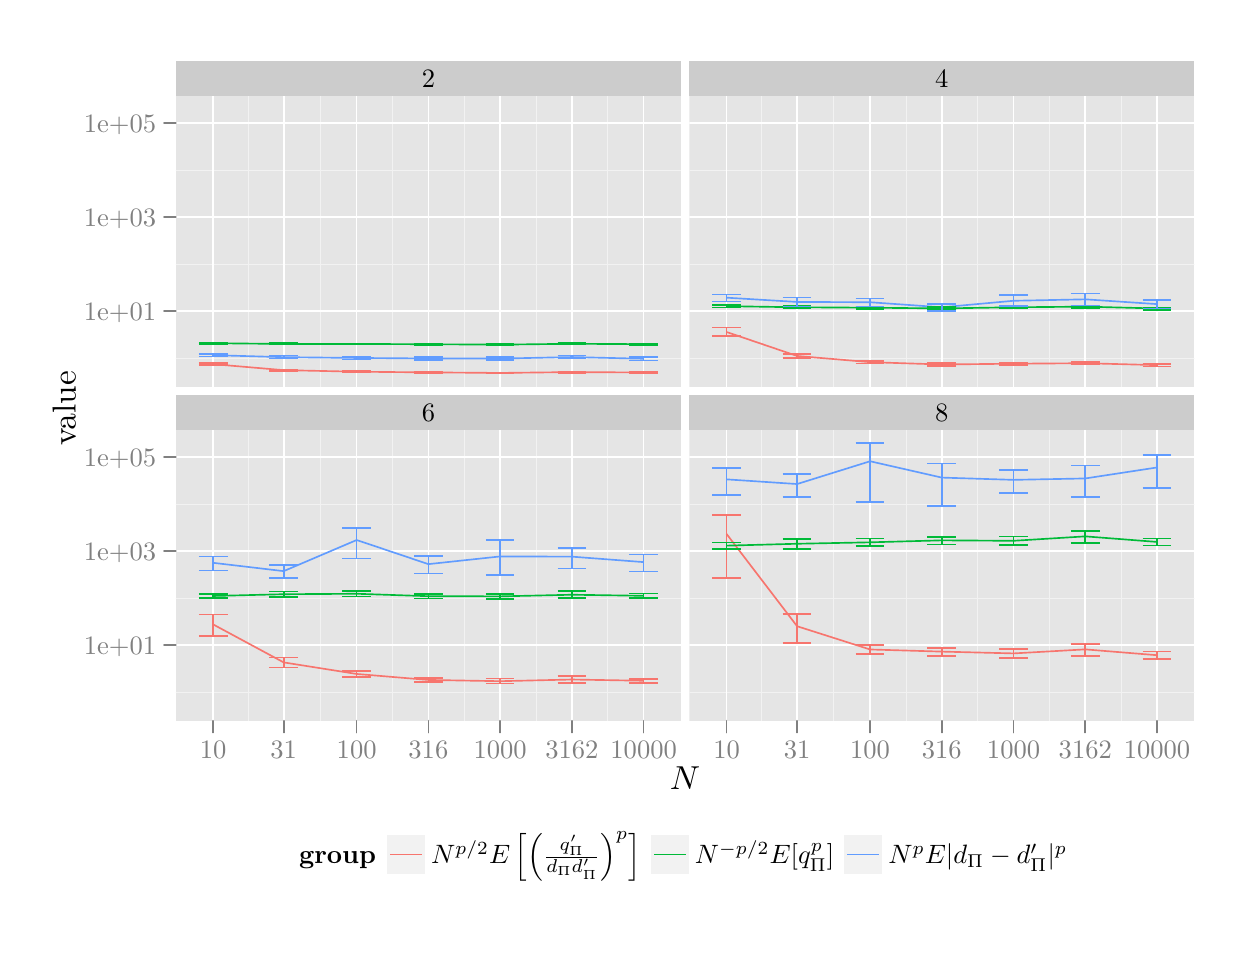
\begin{tikzpicture}[x=1pt,y=1pt]
\definecolor[named]{drawColor}{rgb}{0.00,0.00,0.00}
\definecolor[named]{fillColor}{rgb}{1.00,1.00,1.00}
\fill[color=fillColor,fill opacity=0.00,] (0,0) rectangle (433.62,325.21);
\begin{scope}
\path[clip] (  0.00,  0.00) rectangle (433.62,325.21);
\definecolor[named]{drawColor}{rgb}{0.41,0.16,0.58}
\end{scope}
\begin{scope}
\path[clip] (  0.00,  0.00) rectangle (433.62,325.21);
\definecolor[named]{drawColor}{rgb}{0.41,0.16,0.58}
\end{scope}
\begin{scope}
\path[clip] (  0.00,  0.00) rectangle (433.62,325.21);
\definecolor[named]{drawColor}{rgb}{0.41,0.16,0.58}
\end{scope}
\begin{scope}
\path[clip] (  0.00,  0.00) rectangle (433.62,325.21);
\definecolor[named]{drawColor}{rgb}{0.41,0.16,0.58}
\end{scope}
\begin{scope}
\path[clip] (  0.00,  0.00) rectangle (433.62,325.21);
\definecolor[named]{drawColor}{rgb}{0.41,0.16,0.58}
\end{scope}
\begin{scope}
\path[clip] (  0.00,  0.00) rectangle (433.62,325.21);
\definecolor[named]{drawColor}{rgb}{0.41,0.16,0.58}
\end{scope}
\begin{scope}
\path[clip] (  0.00,  0.00) rectangle (433.62,325.21);
\definecolor[named]{drawColor}{rgb}{0.41,0.16,0.58}
\end{scope}
\begin{scope}
\path[clip] (  0.00,  0.00) rectangle (433.62,325.21);
\definecolor[named]{drawColor}{rgb}{0.41,0.16,0.58}
\end{scope}
\begin{scope}
\path[clip] ( 53.55,195.47) rectangle (236.06,300.54);
\definecolor[named]{drawColor}{rgb}{0.41,0.16,0.58}
\end{scope}
\begin{scope}
\path[clip] (  0.00,  0.00) rectangle (433.62,325.21);
\definecolor[named]{drawColor}{rgb}{0.41,0.16,0.58}
\end{scope}
\begin{scope}
\path[clip] (239.07,195.47) rectangle (421.58,300.54);
\definecolor[named]{drawColor}{rgb}{0.41,0.16,0.58}
\end{scope}
\begin{scope}
\path[clip] (  0.00,  0.00) rectangle (433.62,325.21);
\definecolor[named]{drawColor}{rgb}{0.41,0.16,0.58}
\end{scope}
\begin{scope}
\path[clip] ( 53.55, 74.76) rectangle (236.06,179.83);
\definecolor[named]{drawColor}{rgb}{0.41,0.16,0.58}
\end{scope}
\begin{scope}
\path[clip] (  0.00,  0.00) rectangle (433.62,325.21);
\definecolor[named]{drawColor}{rgb}{0.41,0.16,0.58}
\end{scope}
\begin{scope}
\path[clip] (239.07, 74.76) rectangle (421.58,179.83);
\definecolor[named]{drawColor}{rgb}{0.41,0.16,0.58}
\end{scope}
\begin{scope}
\path[clip] (  0.00,  0.00) rectangle (433.62,325.21);
\definecolor[named]{drawColor}{rgb}{0.41,0.16,0.58}
\end{scope}
\begin{scope}
\path[clip] (  0.00,  0.00) rectangle (433.62,325.21);
\definecolor[named]{drawColor}{rgb}{0.41,0.16,0.58}
\end{scope}
\begin{scope}
\path[clip] (  0.00,  0.00) rectangle (433.62,325.21);
\definecolor[named]{drawColor}{rgb}{0.41,0.16,0.58}
\end{scope}
\begin{scope}
\path[clip] (  0.00,  0.00) rectangle (433.62,325.21);
\definecolor[named]{drawColor}{rgb}{0.41,0.16,0.58}
\end{scope}
\begin{scope}
\path[clip] (  0.00,  0.00) rectangle (433.62,325.21);
\definecolor[named]{drawColor}{rgb}{0.41,0.16,0.58}
\end{scope}
\begin{scope}
\path[clip] (  0.00,  0.00) rectangle (433.62,325.21);
\definecolor[named]{drawColor}{rgb}{0.41,0.16,0.58}
\end{scope}
\begin{scope}
\path[clip] (  0.00,  0.00) rectangle (433.62,325.21);
\definecolor[named]{drawColor}{rgb}{0.41,0.16,0.58}
\end{scope}
\begin{scope}
\path[clip] (  0.00,  0.00) rectangle (433.62,325.21);
\definecolor[named]{drawColor}{rgb}{0.41,0.16,0.58}
\end{scope}
\begin{scope}
\path[clip] (  0.00,  0.00) rectangle (433.62,325.21);
\definecolor[named]{drawColor}{rgb}{0.41,0.16,0.58}
\end{scope}
\begin{scope}
\path[clip] (  0.00,  0.00) rectangle (433.62,325.21);
\definecolor[named]{drawColor}{rgb}{0.41,0.16,0.58}
\end{scope}
\begin{scope}
\path[clip] (  0.00,  0.00) rectangle (433.62,325.21);
\definecolor[named]{drawColor}{rgb}{0.41,0.16,0.58}
\end{scope}
\begin{scope}
\path[clip] (  0.00,  0.00) rectangle (433.62,325.21);
\definecolor[named]{drawColor}{rgb}{0.41,0.16,0.58}
\end{scope}
\begin{scope}
\path[clip] (  0.00,  0.00) rectangle (433.62,325.21);
\definecolor[named]{drawColor}{rgb}{0.41,0.16,0.58}
\end{scope}
\begin{scope}
\path[clip] (  0.00,  0.00) rectangle (433.62,325.21);
\definecolor[named]{drawColor}{rgb}{0.41,0.16,0.58}
\end{scope}
\begin{scope}
\path[clip] (  0.00,  0.00) rectangle (433.62,325.21);
\definecolor[named]{drawColor}{rgb}{0.41,0.16,0.58}
\end{scope}
\begin{scope}
\path[clip] (  0.00,  0.00) rectangle (433.62,325.21);
\definecolor[named]{drawColor}{rgb}{0.41,0.16,0.58}
\end{scope}
\begin{scope}
\path[clip] (  0.00,  0.00) rectangle (433.62,325.21);
\definecolor[named]{drawColor}{rgb}{0.41,0.16,0.58}
\end{scope}
\begin{scope}
\path[clip] (  0.00,  0.00) rectangle (433.62,325.21);
\definecolor[named]{drawColor}{rgb}{0.41,0.16,0.58}
\end{scope}
\begin{scope}
\path[clip] (  0.00,  0.00) rectangle (433.62,325.21);
\definecolor[named]{drawColor}{rgb}{0.41,0.16,0.58}
\end{scope}
\begin{scope}
\path[clip] (  0.00,  0.00) rectangle (433.62,325.21);
\definecolor[named]{drawColor}{rgb}{0.41,0.16,0.58}
\end{scope}
\begin{scope}
\path[clip] (  0.00,  0.00) rectangle (433.62,325.21);
\definecolor[named]{drawColor}{rgb}{0.41,0.16,0.58}
\end{scope}
\begin{scope}
\path[clip] (  0.00,  0.00) rectangle (433.62,325.21);
\definecolor[named]{drawColor}{rgb}{0.41,0.16,0.58}
\end{scope}
\begin{scope}
\path[clip] (  0.00,  0.00) rectangle (433.62,325.21);
\definecolor[named]{drawColor}{rgb}{0.41,0.16,0.58}
\end{scope}
\begin{scope}
\path[clip] (  0.00,  0.00) rectangle (433.62,325.21);
\definecolor[named]{drawColor}{rgb}{0.41,0.16,0.58}
\end{scope}
\begin{scope}
\path[clip] (  0.00,  0.00) rectangle (433.62,325.21);
\definecolor[named]{drawColor}{rgb}{0.41,0.16,0.58}
\end{scope}
\begin{scope}
\path[clip] (  0.00,  0.00) rectangle (433.62,325.21);
\definecolor[named]{drawColor}{rgb}{0.41,0.16,0.58}
\end{scope}
\begin{scope}
\path[clip] (  0.00,  0.00) rectangle (433.62,325.21);
\definecolor[named]{drawColor}{rgb}{0.41,0.16,0.58}
\end{scope}
\begin{scope}
\path[clip] (  0.00,  0.00) rectangle (433.62,325.21);
\definecolor[named]{drawColor}{rgb}{0.41,0.16,0.58}
\end{scope}
\begin{scope}
\path[clip] (  0.00,  0.00) rectangle (433.62,325.21);
\definecolor[named]{drawColor}{rgb}{0.41,0.16,0.58}
\end{scope}
\begin{scope}
\path[clip] (  0.00,  0.00) rectangle (433.62,325.21);
\definecolor[named]{drawColor}{rgb}{0.41,0.16,0.58}
\end{scope}
\begin{scope}
\path[clip] (  0.00,  0.00) rectangle (433.62,325.21);
\definecolor[named]{drawColor}{rgb}{0.41,0.16,0.58}
\end{scope}
\begin{scope}
\path[clip] (  0.00,  0.00) rectangle (433.62,325.21);
\definecolor[named]{drawColor}{rgb}{0.41,0.16,0.58}
\end{scope}
\begin{scope}
\path[clip] (  0.00,  0.00) rectangle (433.62,325.21);
\definecolor[named]{drawColor}{rgb}{0.41,0.16,0.58}
\end{scope}
\begin{scope}
\path[clip] (  0.00,  0.00) rectangle (433.62,325.21);
\definecolor[named]{drawColor}{rgb}{0.41,0.16,0.58}
\definecolor[named]{fillColor}{rgb}{1.00,1.00,1.00}

\draw[fill=fillColor,draw opacity=0.00,] (  0.00,  0.00) rectangle (433.62,325.21);
\end{scope}
\begin{scope}
\path[clip] (  0.00,  0.00) rectangle (433.62,325.21);
\definecolor[named]{drawColor}{rgb}{0.41,0.16,0.58}
\end{scope}
\begin{scope}
\path[clip] ( 53.55,195.47) rectangle (236.06,300.54);
\definecolor[named]{drawColor}{rgb}{0.41,0.16,0.58}
\definecolor[named]{fillColor}{rgb}{0.90,0.90,0.90}

\draw[fill=fillColor,draw opacity=0.00,] ( 53.55,195.47) rectangle (236.06,300.54);
\definecolor[named]{drawColor}{rgb}{0.95,0.95,0.95}

\draw[color=drawColor,line width= 0.3pt,line cap=round,line join=round,fill opacity=0.00,] ( 53.55,205.77) --
	(236.06,205.77);

\draw[color=drawColor,line width= 0.3pt,line cap=round,line join=round,fill opacity=0.00,] ( 53.55,239.78) --
	(236.06,239.78);

\draw[color=drawColor,line width= 0.3pt,line cap=round,line join=round,fill opacity=0.00,] ( 53.55,273.79) --
	(236.06,273.79);

\draw[color=drawColor,line width= 0.3pt,line cap=round,line join=round,fill opacity=0.00,] ( 79.77,195.47) --
	( 79.77,300.54);

\draw[color=drawColor,line width= 0.3pt,line cap=round,line join=round,fill opacity=0.00,] (105.69,195.47) --
	(105.69,300.54);

\draw[color=drawColor,line width= 0.3pt,line cap=round,line join=round,fill opacity=0.00,] (131.83,195.47) --
	(131.83,300.54);

\draw[color=drawColor,line width= 0.3pt,line cap=round,line join=round,fill opacity=0.00,] (157.76,195.47) --
	(157.76,300.54);

\draw[color=drawColor,line width= 0.3pt,line cap=round,line join=round,fill opacity=0.00,] (183.69,195.47) --
	(183.69,300.54);

\draw[color=drawColor,line width= 0.3pt,line cap=round,line join=round,fill opacity=0.00,] (209.61,195.47) --
	(209.61,300.54);
\definecolor[named]{drawColor}{rgb}{1.00,1.00,1.00}

\draw[color=drawColor,line width= 0.6pt,line cap=round,line join=round,fill opacity=0.00,] ( 53.55,222.77) --
	(236.06,222.77);

\draw[color=drawColor,line width= 0.6pt,line cap=round,line join=round,fill opacity=0.00,] ( 53.55,256.78) --
	(236.06,256.78);

\draw[color=drawColor,line width= 0.6pt,line cap=round,line join=round,fill opacity=0.00,] ( 53.55,290.80) --
	(236.06,290.80);

\draw[color=drawColor,line width= 0.6pt,line cap=round,line join=round,fill opacity=0.00,] ( 67.03,195.47) --
	( 67.03,300.54);

\draw[color=drawColor,line width= 0.6pt,line cap=round,line join=round,fill opacity=0.00,] ( 92.51,195.47) --
	( 92.51,300.54);

\draw[color=drawColor,line width= 0.6pt,line cap=round,line join=round,fill opacity=0.00,] (118.88,195.47) --
	(118.88,300.54);

\draw[color=drawColor,line width= 0.6pt,line cap=round,line join=round,fill opacity=0.00,] (144.79,195.47) --
	(144.79,300.54);

\draw[color=drawColor,line width= 0.6pt,line cap=round,line join=round,fill opacity=0.00,] (170.73,195.47) --
	(170.73,300.54);

\draw[color=drawColor,line width= 0.6pt,line cap=round,line join=round,fill opacity=0.00,] (196.65,195.47) --
	(196.65,300.54);

\draw[color=drawColor,line width= 0.6pt,line cap=round,line join=round,fill opacity=0.00,] (222.58,195.47) --
	(222.58,300.54);
\definecolor[named]{drawColor}{rgb}{0.97,0.46,0.43}

\draw[color=drawColor,line width= 0.6pt,line join=round,fill opacity=0.00,] ( 67.03,203.62) --
	( 92.51,201.45) --
	(118.88,200.89) --
	(144.79,200.64) --
	(170.73,200.45) --
	(196.65,200.75) --
	(222.58,200.61);
\definecolor[named]{drawColor}{rgb}{0.00,0.73,0.22}

\draw[color=drawColor,line width= 0.6pt,line join=round,fill opacity=0.00,] ( 67.03,211.18) --
	( 92.51,210.93) --
	(118.88,210.93) --
	(144.79,210.81) --
	(170.73,210.67) --
	(196.65,210.98) --
	(222.58,210.84);
\definecolor[named]{drawColor}{rgb}{0.38,0.61,1.00}

\draw[color=drawColor,line width= 0.6pt,line join=round,fill opacity=0.00,] ( 67.03,206.87) --
	( 92.51,206.15) --
	(118.88,205.86) --
	(144.79,205.67) --
	(170.73,205.63) --
	(196.65,206.19) --
	(222.58,205.57);
\definecolor[named]{drawColor}{rgb}{0.97,0.46,0.43}

\draw[color=drawColor,line width= 0.6pt,line join=round,fill opacity=0.00,] ( 61.85,203.97) --
	( 72.22,203.97);

\draw[color=drawColor,line width= 0.6pt,line join=round,fill opacity=0.00,] ( 67.03,203.97) --
	( 67.03,203.29);

\draw[color=drawColor,line width= 0.6pt,line join=round,fill opacity=0.00,] ( 61.85,203.29) --
	( 72.22,203.29);

\draw[color=drawColor,line width= 0.6pt,line join=round,fill opacity=0.00,] ( 87.32,201.67) --
	( 97.69,201.67);

\draw[color=drawColor,line width= 0.6pt,line join=round,fill opacity=0.00,] ( 92.51,201.67) --
	( 92.51,201.22);

\draw[color=drawColor,line width= 0.6pt,line join=round,fill opacity=0.00,] ( 87.32,201.22) --
	( 97.69,201.22);

\draw[color=drawColor,line width= 0.6pt,line join=round,fill opacity=0.00,] (113.69,201.09) --
	(124.06,201.09);

\draw[color=drawColor,line width= 0.6pt,line join=round,fill opacity=0.00,] (118.88,201.09) --
	(118.88,200.69);

\draw[color=drawColor,line width= 0.6pt,line join=round,fill opacity=0.00,] (113.69,200.69) --
	(124.06,200.69);

\draw[color=drawColor,line width= 0.6pt,line join=round,fill opacity=0.00,] (139.60,200.84) --
	(149.97,200.84);

\draw[color=drawColor,line width= 0.6pt,line join=round,fill opacity=0.00,] (144.79,200.84) --
	(144.79,200.43);

\draw[color=drawColor,line width= 0.6pt,line join=round,fill opacity=0.00,] (139.60,200.43) --
	(149.97,200.43);

\draw[color=drawColor,line width= 0.6pt,line join=round,fill opacity=0.00,] (165.54,200.66) --
	(175.91,200.66);

\draw[color=drawColor,line width= 0.6pt,line join=round,fill opacity=0.00,] (170.73,200.66) --
	(170.73,200.25);

\draw[color=drawColor,line width= 0.6pt,line join=round,fill opacity=0.00,] (165.54,200.25) --
	(175.91,200.25);

\draw[color=drawColor,line width= 0.6pt,line join=round,fill opacity=0.00,] (191.47,200.94) --
	(201.83,200.94);

\draw[color=drawColor,line width= 0.6pt,line join=round,fill opacity=0.00,] (196.65,200.94) --
	(196.65,200.54);

\draw[color=drawColor,line width= 0.6pt,line join=round,fill opacity=0.00,] (191.47,200.54) --
	(201.83,200.54);

\draw[color=drawColor,line width= 0.6pt,line join=round,fill opacity=0.00,] (217.39,200.82) --
	(227.76,200.82);

\draw[color=drawColor,line width= 0.6pt,line join=round,fill opacity=0.00,] (222.58,200.82) --
	(222.58,200.41);

\draw[color=drawColor,line width= 0.6pt,line join=round,fill opacity=0.00,] (217.39,200.41) --
	(227.76,200.41);
\definecolor[named]{drawColor}{rgb}{0.00,0.73,0.22}

\draw[color=drawColor,line width= 0.6pt,line join=round,fill opacity=0.00,] ( 61.85,211.38) --
	( 72.22,211.38);

\draw[color=drawColor,line width= 0.6pt,line join=round,fill opacity=0.00,] ( 67.03,211.38) --
	( 67.03,210.97);

\draw[color=drawColor,line width= 0.6pt,line join=round,fill opacity=0.00,] ( 61.85,210.97) --
	( 72.22,210.97);

\draw[color=drawColor,line width= 0.6pt,line join=round,fill opacity=0.00,] ( 87.32,211.15) --
	( 97.69,211.15);

\draw[color=drawColor,line width= 0.6pt,line join=round,fill opacity=0.00,] ( 92.51,211.15) --
	( 92.51,210.73);

\draw[color=drawColor,line width= 0.6pt,line join=round,fill opacity=0.00,] ( 87.32,210.73) --
	( 97.69,210.73);

\draw[color=drawColor,line width= 0.6pt,line join=round,fill opacity=0.00,] (113.69,211.12) --
	(124.06,211.12);

\draw[color=drawColor,line width= 0.6pt,line join=round,fill opacity=0.00,] (118.88,211.12) --
	(118.88,210.73);

\draw[color=drawColor,line width= 0.6pt,line join=round,fill opacity=0.00,] (113.69,210.73) --
	(124.06,210.73);

\draw[color=drawColor,line width= 0.6pt,line join=round,fill opacity=0.00,] (139.60,210.99) --
	(149.97,210.99);

\draw[color=drawColor,line width= 0.6pt,line join=round,fill opacity=0.00,] (144.79,210.99) --
	(144.79,210.60);

\draw[color=drawColor,line width= 0.6pt,line join=round,fill opacity=0.00,] (139.60,210.60) --
	(149.97,210.60);

\draw[color=drawColor,line width= 0.6pt,line join=round,fill opacity=0.00,] (165.54,210.86) --
	(175.91,210.86);

\draw[color=drawColor,line width= 0.6pt,line join=round,fill opacity=0.00,] (170.73,210.86) --
	(170.73,210.48);

\draw[color=drawColor,line width= 0.6pt,line join=round,fill opacity=0.00,] (165.54,210.48) --
	(175.91,210.48);

\draw[color=drawColor,line width= 0.6pt,line join=round,fill opacity=0.00,] (191.47,211.18) --
	(201.83,211.18);

\draw[color=drawColor,line width= 0.6pt,line join=round,fill opacity=0.00,] (196.65,211.18) --
	(196.65,210.77);

\draw[color=drawColor,line width= 0.6pt,line join=round,fill opacity=0.00,] (191.47,210.77) --
	(201.83,210.77);

\draw[color=drawColor,line width= 0.6pt,line join=round,fill opacity=0.00,] (217.39,211.05) --
	(227.76,211.05);

\draw[color=drawColor,line width= 0.6pt,line join=round,fill opacity=0.00,] (222.58,211.05) --
	(222.58,210.63);

\draw[color=drawColor,line width= 0.6pt,line join=round,fill opacity=0.00,] (217.39,210.63) --
	(227.76,210.63);
\definecolor[named]{drawColor}{rgb}{0.38,0.61,1.00}

\draw[color=drawColor,line width= 0.6pt,line join=round,fill opacity=0.00,] ( 61.85,207.36) --
	( 72.22,207.36);

\draw[color=drawColor,line width= 0.6pt,line join=round,fill opacity=0.00,] ( 67.03,207.36) --
	( 67.03,206.33);

\draw[color=drawColor,line width= 0.6pt,line join=round,fill opacity=0.00,] ( 61.85,206.33) --
	( 72.22,206.33);

\draw[color=drawColor,line width= 0.6pt,line join=round,fill opacity=0.00,] ( 87.32,206.72) --
	( 97.69,206.72);

\draw[color=drawColor,line width= 0.6pt,line join=round,fill opacity=0.00,] ( 92.51,206.72) --
	( 92.51,205.63);

\draw[color=drawColor,line width= 0.6pt,line join=round,fill opacity=0.00,] ( 87.32,205.63) --
	( 97.69,205.63);

\draw[color=drawColor,line width= 0.6pt,line join=round,fill opacity=0.00,] (113.69,206.40) --
	(124.06,206.40);

\draw[color=drawColor,line width= 0.6pt,line join=round,fill opacity=0.00,] (118.88,206.40) --
	(118.88,205.30);

\draw[color=drawColor,line width= 0.6pt,line join=round,fill opacity=0.00,] (113.69,205.30) --
	(124.06,205.30);

\draw[color=drawColor,line width= 0.6pt,line join=round,fill opacity=0.00,] (139.60,206.17) --
	(149.97,206.17);

\draw[color=drawColor,line width= 0.6pt,line join=round,fill opacity=0.00,] (144.79,206.17) --
	(144.79,205.15);

\draw[color=drawColor,line width= 0.6pt,line join=round,fill opacity=0.00,] (139.60,205.15) --
	(149.97,205.15);

\draw[color=drawColor,line width= 0.6pt,line join=round,fill opacity=0.00,] (165.54,206.23) --
	(175.91,206.23);

\draw[color=drawColor,line width= 0.6pt,line join=round,fill opacity=0.00,] (170.73,206.23) --
	(170.73,205.01);

\draw[color=drawColor,line width= 0.6pt,line join=round,fill opacity=0.00,] (165.54,205.01) --
	(175.91,205.01);

\draw[color=drawColor,line width= 0.6pt,line join=round,fill opacity=0.00,] (191.47,206.74) --
	(201.83,206.74);

\draw[color=drawColor,line width= 0.6pt,line join=round,fill opacity=0.00,] (196.65,206.74) --
	(196.65,205.64);

\draw[color=drawColor,line width= 0.6pt,line join=round,fill opacity=0.00,] (191.47,205.64) --
	(201.83,205.64);

\draw[color=drawColor,line width= 0.6pt,line join=round,fill opacity=0.00,] (217.39,206.21) --
	(227.76,206.21);

\draw[color=drawColor,line width= 0.6pt,line join=round,fill opacity=0.00,] (222.58,206.21) --
	(222.58,204.91);

\draw[color=drawColor,line width= 0.6pt,line join=round,fill opacity=0.00,] (217.39,204.91) --
	(227.76,204.91);
\end{scope}
\begin{scope}
\path[clip] (  0.00,  0.00) rectangle (433.62,325.21);
\definecolor[named]{drawColor}{rgb}{0.41,0.16,0.58}
\end{scope}
\begin{scope}
\path[clip] (239.07,195.47) rectangle (421.58,300.54);
\definecolor[named]{drawColor}{rgb}{0.41,0.16,0.58}
\definecolor[named]{fillColor}{rgb}{0.90,0.90,0.90}

\draw[fill=fillColor,draw opacity=0.00,] (239.07,195.47) rectangle (421.57,300.54);
\definecolor[named]{drawColor}{rgb}{0.95,0.95,0.95}

\draw[color=drawColor,line width= 0.3pt,line cap=round,line join=round,fill opacity=0.00,] (239.07,205.77) --
	(421.58,205.77);

\draw[color=drawColor,line width= 0.3pt,line cap=round,line join=round,fill opacity=0.00,] (239.07,239.78) --
	(421.58,239.78);

\draw[color=drawColor,line width= 0.3pt,line cap=round,line join=round,fill opacity=0.00,] (239.07,273.79) --
	(421.58,273.79);

\draw[color=drawColor,line width= 0.3pt,line cap=round,line join=round,fill opacity=0.00,] (265.29,195.47) --
	(265.29,300.54);

\draw[color=drawColor,line width= 0.3pt,line cap=round,line join=round,fill opacity=0.00,] (291.21,195.47) --
	(291.21,300.54);

\draw[color=drawColor,line width= 0.3pt,line cap=round,line join=round,fill opacity=0.00,] (317.35,195.47) --
	(317.35,300.54);

\draw[color=drawColor,line width= 0.3pt,line cap=round,line join=round,fill opacity=0.00,] (343.28,195.47) --
	(343.28,300.54);

\draw[color=drawColor,line width= 0.3pt,line cap=round,line join=round,fill opacity=0.00,] (369.21,195.47) --
	(369.21,300.54);

\draw[color=drawColor,line width= 0.3pt,line cap=round,line join=round,fill opacity=0.00,] (395.13,195.47) --
	(395.13,300.54);
\definecolor[named]{drawColor}{rgb}{1.00,1.00,1.00}

\draw[color=drawColor,line width= 0.6pt,line cap=round,line join=round,fill opacity=0.00,] (239.07,222.77) --
	(421.58,222.77);

\draw[color=drawColor,line width= 0.6pt,line cap=round,line join=round,fill opacity=0.00,] (239.07,256.78) --
	(421.58,256.78);

\draw[color=drawColor,line width= 0.6pt,line cap=round,line join=round,fill opacity=0.00,] (239.07,290.80) --
	(421.58,290.80);

\draw[color=drawColor,line width= 0.6pt,line cap=round,line join=round,fill opacity=0.00,] (252.55,195.47) --
	(252.55,300.54);

\draw[color=drawColor,line width= 0.6pt,line cap=round,line join=round,fill opacity=0.00,] (278.03,195.47) --
	(278.03,300.54);

\draw[color=drawColor,line width= 0.6pt,line cap=round,line join=round,fill opacity=0.00,] (304.40,195.47) --
	(304.40,300.54);

\draw[color=drawColor,line width= 0.6pt,line cap=round,line join=round,fill opacity=0.00,] (330.31,195.47) --
	(330.31,300.54);

\draw[color=drawColor,line width= 0.6pt,line cap=round,line join=round,fill opacity=0.00,] (356.25,195.47) --
	(356.25,300.54);

\draw[color=drawColor,line width= 0.6pt,line cap=round,line join=round,fill opacity=0.00,] (382.17,195.47) --
	(382.17,300.54);

\draw[color=drawColor,line width= 0.6pt,line cap=round,line join=round,fill opacity=0.00,] (408.09,195.47) --
	(408.09,300.54);
\definecolor[named]{drawColor}{rgb}{0.97,0.46,0.43}

\draw[color=drawColor,line width= 0.6pt,line join=round,fill opacity=0.00,] (252.55,215.24) --
	(278.03,206.58) --
	(304.40,204.34) --
	(330.31,203.50) --
	(356.25,203.78) --
	(382.17,203.96) --
	(408.09,203.27);
\definecolor[named]{drawColor}{rgb}{0.00,0.73,0.22}

\draw[color=drawColor,line width= 0.6pt,line join=round,fill opacity=0.00,] (252.55,224.58) --
	(278.03,224.17) --
	(304.40,224.02) --
	(330.31,223.76) --
	(356.25,224.17) --
	(382.17,224.40) --
	(408.09,223.74);
\definecolor[named]{drawColor}{rgb}{0.38,0.61,1.00}

\draw[color=drawColor,line width= 0.6pt,line join=round,fill opacity=0.00,] (252.55,227.64) --
	(278.03,226.10) --
	(304.40,225.99) --
	(330.31,224.17) --
	(356.25,226.52) --
	(382.17,227.04) --
	(408.09,225.32);
\definecolor[named]{drawColor}{rgb}{0.97,0.46,0.43}

\draw[color=drawColor,line width= 0.6pt,line join=round,fill opacity=0.00,] (247.36,216.84) --
	(257.73,216.84);

\draw[color=drawColor,line width= 0.6pt,line join=round,fill opacity=0.00,] (252.55,216.84) --
	(252.55,213.69);

\draw[color=drawColor,line width= 0.6pt,line join=round,fill opacity=0.00,] (247.36,213.69) --
	(257.73,213.69);

\draw[color=drawColor,line width= 0.6pt,line join=round,fill opacity=0.00,] (272.84,207.32) --
	(283.21,207.32);

\draw[color=drawColor,line width= 0.6pt,line join=round,fill opacity=0.00,] (278.03,207.32) --
	(278.03,205.85);

\draw[color=drawColor,line width= 0.6pt,line join=round,fill opacity=0.00,] (272.84,205.85) --
	(283.21,205.85);

\draw[color=drawColor,line width= 0.6pt,line join=round,fill opacity=0.00,] (299.21,204.83) --
	(309.58,204.83);

\draw[color=drawColor,line width= 0.6pt,line join=round,fill opacity=0.00,] (304.40,204.83) --
	(304.40,203.84);

\draw[color=drawColor,line width= 0.6pt,line join=round,fill opacity=0.00,] (299.21,203.84) --
	(309.58,203.84);

\draw[color=drawColor,line width= 0.6pt,line join=round,fill opacity=0.00,] (325.12,204.01) --
	(335.49,204.01);

\draw[color=drawColor,line width= 0.6pt,line join=round,fill opacity=0.00,] (330.31,204.01) --
	(330.31,202.98);

\draw[color=drawColor,line width= 0.6pt,line join=round,fill opacity=0.00,] (325.12,202.98) --
	(335.49,202.98);

\draw[color=drawColor,line width= 0.6pt,line join=round,fill opacity=0.00,] (351.06,204.24) --
	(361.43,204.24);

\draw[color=drawColor,line width= 0.6pt,line join=round,fill opacity=0.00,] (356.25,204.24) --
	(356.25,203.27);

\draw[color=drawColor,line width= 0.6pt,line join=round,fill opacity=0.00,] (351.06,203.27) --
	(361.43,203.27);

\draw[color=drawColor,line width= 0.6pt,line join=round,fill opacity=0.00,] (376.98,204.43) --
	(387.35,204.43);

\draw[color=drawColor,line width= 0.6pt,line join=round,fill opacity=0.00,] (382.17,204.43) --
	(382.17,203.49);

\draw[color=drawColor,line width= 0.6pt,line join=round,fill opacity=0.00,] (376.98,203.49) --
	(387.35,203.49);

\draw[color=drawColor,line width= 0.6pt,line join=round,fill opacity=0.00,] (402.91,203.72) --
	(413.28,203.72);

\draw[color=drawColor,line width= 0.6pt,line join=round,fill opacity=0.00,] (408.09,203.72) --
	(408.09,202.82);

\draw[color=drawColor,line width= 0.6pt,line join=round,fill opacity=0.00,] (402.91,202.82) --
	(413.28,202.82);
\definecolor[named]{drawColor}{rgb}{0.00,0.73,0.22}

\draw[color=drawColor,line width= 0.6pt,line join=round,fill opacity=0.00,] (247.36,224.99) --
	(257.73,224.99);

\draw[color=drawColor,line width= 0.6pt,line join=round,fill opacity=0.00,] (252.55,224.99) --
	(252.55,224.14);

\draw[color=drawColor,line width= 0.6pt,line join=round,fill opacity=0.00,] (247.36,224.14) --
	(257.73,224.14);

\draw[color=drawColor,line width= 0.6pt,line join=round,fill opacity=0.00,] (272.84,224.65) --
	(283.21,224.65);

\draw[color=drawColor,line width= 0.6pt,line join=round,fill opacity=0.00,] (278.03,224.65) --
	(278.03,223.69);

\draw[color=drawColor,line width= 0.6pt,line join=round,fill opacity=0.00,] (272.84,223.69) --
	(283.21,223.69);

\draw[color=drawColor,line width= 0.6pt,line join=round,fill opacity=0.00,] (299.21,224.44) --
	(309.58,224.44);

\draw[color=drawColor,line width= 0.6pt,line join=round,fill opacity=0.00,] (304.40,224.44) --
	(304.40,223.57);

\draw[color=drawColor,line width= 0.6pt,line join=round,fill opacity=0.00,] (299.21,223.57) --
	(309.58,223.57);

\draw[color=drawColor,line width= 0.6pt,line join=round,fill opacity=0.00,] (325.12,224.26) --
	(335.49,224.26);

\draw[color=drawColor,line width= 0.6pt,line join=round,fill opacity=0.00,] (330.31,224.26) --
	(330.31,223.28);

\draw[color=drawColor,line width= 0.6pt,line join=round,fill opacity=0.00,] (325.12,223.28) --
	(335.49,223.28);

\draw[color=drawColor,line width= 0.6pt,line join=round,fill opacity=0.00,] (351.06,224.62) --
	(361.43,224.62);

\draw[color=drawColor,line width= 0.6pt,line join=round,fill opacity=0.00,] (356.25,224.62) --
	(356.25,223.69);

\draw[color=drawColor,line width= 0.6pt,line join=round,fill opacity=0.00,] (351.06,223.69) --
	(361.43,223.69);

\draw[color=drawColor,line width= 0.6pt,line join=round,fill opacity=0.00,] (376.98,224.86) --
	(387.35,224.86);

\draw[color=drawColor,line width= 0.6pt,line join=round,fill opacity=0.00,] (382.17,224.86) --
	(382.17,223.93);

\draw[color=drawColor,line width= 0.6pt,line join=round,fill opacity=0.00,] (376.98,223.93) --
	(387.35,223.93);

\draw[color=drawColor,line width= 0.6pt,line join=round,fill opacity=0.00,] (402.91,224.15) --
	(413.28,224.15);

\draw[color=drawColor,line width= 0.6pt,line join=round,fill opacity=0.00,] (408.09,224.15) --
	(408.09,223.29);

\draw[color=drawColor,line width= 0.6pt,line join=round,fill opacity=0.00,] (402.91,223.29) --
	(413.28,223.29);
\definecolor[named]{drawColor}{rgb}{0.38,0.61,1.00}

\draw[color=drawColor,line width= 0.6pt,line join=round,fill opacity=0.00,] (247.36,228.81) --
	(257.73,228.81);

\draw[color=drawColor,line width= 0.6pt,line join=round,fill opacity=0.00,] (252.55,228.81) --
	(252.55,226.29);

\draw[color=drawColor,line width= 0.6pt,line join=round,fill opacity=0.00,] (247.36,226.29) --
	(257.73,226.29);

\draw[color=drawColor,line width= 0.6pt,line join=round,fill opacity=0.00,] (272.84,227.66) --
	(283.21,227.66);

\draw[color=drawColor,line width= 0.6pt,line join=round,fill opacity=0.00,] (278.03,227.66) --
	(278.03,224.40);

\draw[color=drawColor,line width= 0.6pt,line join=round,fill opacity=0.00,] (272.84,224.40) --
	(283.21,224.40);

\draw[color=drawColor,line width= 0.6pt,line join=round,fill opacity=0.00,] (299.21,227.34) --
	(309.58,227.34);

\draw[color=drawColor,line width= 0.6pt,line join=round,fill opacity=0.00,] (304.40,227.34) --
	(304.40,224.49);

\draw[color=drawColor,line width= 0.6pt,line join=round,fill opacity=0.00,] (299.21,224.49) --
	(309.58,224.49);

\draw[color=drawColor,line width= 0.6pt,line join=round,fill opacity=0.00,] (325.12,225.43) --
	(335.49,225.43);

\draw[color=drawColor,line width= 0.6pt,line join=round,fill opacity=0.00,] (330.31,225.43) --
	(330.31,222.87);

\draw[color=drawColor,line width= 0.6pt,line join=round,fill opacity=0.00,] (325.12,222.87) --
	(335.49,222.87);

\draw[color=drawColor,line width= 0.6pt,line join=round,fill opacity=0.00,] (351.06,228.49) --
	(361.43,228.49);

\draw[color=drawColor,line width= 0.6pt,line join=round,fill opacity=0.00,] (356.25,228.49) --
	(356.25,224.54);

\draw[color=drawColor,line width= 0.6pt,line join=round,fill opacity=0.00,] (351.06,224.54) --
	(361.43,224.54);

\draw[color=drawColor,line width= 0.6pt,line join=round,fill opacity=0.00,] (376.98,229.16) --
	(387.35,229.16);

\draw[color=drawColor,line width= 0.6pt,line join=round,fill opacity=0.00,] (382.17,229.16) --
	(382.17,224.82);

\draw[color=drawColor,line width= 0.6pt,line join=round,fill opacity=0.00,] (376.98,224.82) --
	(387.35,224.82);

\draw[color=drawColor,line width= 0.6pt,line join=round,fill opacity=0.00,] (402.91,226.88) --
	(413.28,226.88);

\draw[color=drawColor,line width= 0.6pt,line join=round,fill opacity=0.00,] (408.09,226.88) --
	(408.09,223.76);

\draw[color=drawColor,line width= 0.6pt,line join=round,fill opacity=0.00,] (402.91,223.76) --
	(413.28,223.76);
\end{scope}
\begin{scope}
\path[clip] (  0.00,  0.00) rectangle (433.62,325.21);
\definecolor[named]{drawColor}{rgb}{0.41,0.16,0.58}
\end{scope}
\begin{scope}
\path[clip] ( 53.55, 74.76) rectangle (236.06,179.83);
\definecolor[named]{drawColor}{rgb}{0.41,0.16,0.58}
\definecolor[named]{fillColor}{rgb}{0.90,0.90,0.90}

\draw[fill=fillColor,draw opacity=0.00,] ( 53.55, 74.76) rectangle (236.06,179.83);
\definecolor[named]{drawColor}{rgb}{0.95,0.95,0.95}

\draw[color=drawColor,line width= 0.3pt,line cap=round,line join=round,fill opacity=0.00,] ( 53.55, 85.06) --
	(236.06, 85.06);

\draw[color=drawColor,line width= 0.3pt,line cap=round,line join=round,fill opacity=0.00,] ( 53.55,119.07) --
	(236.06,119.07);

\draw[color=drawColor,line width= 0.3pt,line cap=round,line join=round,fill opacity=0.00,] ( 53.55,153.08) --
	(236.06,153.08);

\draw[color=drawColor,line width= 0.3pt,line cap=round,line join=round,fill opacity=0.00,] ( 79.77, 74.76) --
	( 79.77,179.83);

\draw[color=drawColor,line width= 0.3pt,line cap=round,line join=round,fill opacity=0.00,] (105.69, 74.76) --
	(105.69,179.83);

\draw[color=drawColor,line width= 0.3pt,line cap=round,line join=round,fill opacity=0.00,] (131.83, 74.76) --
	(131.83,179.83);

\draw[color=drawColor,line width= 0.3pt,line cap=round,line join=round,fill opacity=0.00,] (157.76, 74.76) --
	(157.76,179.83);

\draw[color=drawColor,line width= 0.3pt,line cap=round,line join=round,fill opacity=0.00,] (183.69, 74.76) --
	(183.69,179.83);

\draw[color=drawColor,line width= 0.3pt,line cap=round,line join=round,fill opacity=0.00,] (209.61, 74.76) --
	(209.61,179.83);
\definecolor[named]{drawColor}{rgb}{1.00,1.00,1.00}

\draw[color=drawColor,line width= 0.6pt,line cap=round,line join=round,fill opacity=0.00,] ( 53.55,102.06) --
	(236.06,102.06);

\draw[color=drawColor,line width= 0.6pt,line cap=round,line join=round,fill opacity=0.00,] ( 53.55,136.07) --
	(236.06,136.07);

\draw[color=drawColor,line width= 0.6pt,line cap=round,line join=round,fill opacity=0.00,] ( 53.55,170.09) --
	(236.06,170.09);

\draw[color=drawColor,line width= 0.6pt,line cap=round,line join=round,fill opacity=0.00,] ( 67.03, 74.76) --
	( 67.03,179.83);

\draw[color=drawColor,line width= 0.6pt,line cap=round,line join=round,fill opacity=0.00,] ( 92.51, 74.76) --
	( 92.51,179.83);

\draw[color=drawColor,line width= 0.6pt,line cap=round,line join=round,fill opacity=0.00,] (118.88, 74.76) --
	(118.88,179.83);

\draw[color=drawColor,line width= 0.6pt,line cap=round,line join=round,fill opacity=0.00,] (144.79, 74.76) --
	(144.79,179.83);

\draw[color=drawColor,line width= 0.6pt,line cap=round,line join=round,fill opacity=0.00,] (170.73, 74.76) --
	(170.73,179.83);

\draw[color=drawColor,line width= 0.6pt,line cap=round,line join=round,fill opacity=0.00,] (196.65, 74.76) --
	(196.65,179.83);

\draw[color=drawColor,line width= 0.6pt,line cap=round,line join=round,fill opacity=0.00,] (222.58, 74.76) --
	(222.58,179.83);
\definecolor[named]{drawColor}{rgb}{0.97,0.46,0.43}

\draw[color=drawColor,line width= 0.6pt,line join=round,fill opacity=0.00,] ( 67.03,109.57) --
	( 92.51, 95.85) --
	(118.88, 91.67) --
	(144.79, 89.51) --
	(170.73, 89.06) --
	(196.65, 89.66) --
	(222.58, 89.22);
\definecolor[named]{drawColor}{rgb}{0.00,0.73,0.22}

\draw[color=drawColor,line width= 0.6pt,line join=round,fill opacity=0.00,] ( 67.03,119.85) --
	( 92.51,120.49) --
	(118.88,120.65) --
	(144.79,119.77) --
	(170.73,119.71) --
	(196.65,120.30) --
	(222.58,119.91);
\definecolor[named]{drawColor}{rgb}{0.38,0.61,1.00}

\draw[color=drawColor,line width= 0.6pt,line join=round,fill opacity=0.00,] ( 67.03,131.83) --
	( 92.51,128.83) --
	(118.88,140.07) --
	(144.79,131.36) --
	(170.73,134.14) --
	(196.65,134.06) --
	(222.58,132.09);
\definecolor[named]{drawColor}{rgb}{0.97,0.46,0.43}

\draw[color=drawColor,line width= 0.6pt,line join=round,fill opacity=0.00,] ( 61.85,113.19) --
	( 72.22,113.19);

\draw[color=drawColor,line width= 0.6pt,line join=round,fill opacity=0.00,] ( 67.03,113.19) --
	( 67.03,105.42);

\draw[color=drawColor,line width= 0.6pt,line join=round,fill opacity=0.00,] ( 61.85,105.42) --
	( 72.22,105.42);

\draw[color=drawColor,line width= 0.6pt,line join=round,fill opacity=0.00,] ( 87.32, 97.57) --
	( 97.69, 97.57);

\draw[color=drawColor,line width= 0.6pt,line join=round,fill opacity=0.00,] ( 92.51, 97.57) --
	( 92.51, 94.02);

\draw[color=drawColor,line width= 0.6pt,line join=round,fill opacity=0.00,] ( 87.32, 94.02) --
	( 97.69, 94.02);

\draw[color=drawColor,line width= 0.6pt,line join=round,fill opacity=0.00,] (113.69, 92.72) --
	(124.06, 92.72);

\draw[color=drawColor,line width= 0.6pt,line join=round,fill opacity=0.00,] (118.88, 92.72) --
	(118.88, 90.62);

\draw[color=drawColor,line width= 0.6pt,line join=round,fill opacity=0.00,] (113.69, 90.62) --
	(124.06, 90.62);

\draw[color=drawColor,line width= 0.6pt,line join=round,fill opacity=0.00,] (139.60, 90.31) --
	(149.97, 90.31);

\draw[color=drawColor,line width= 0.6pt,line join=round,fill opacity=0.00,] (144.79, 90.31) --
	(144.79, 88.73);

\draw[color=drawColor,line width= 0.6pt,line join=round,fill opacity=0.00,] (139.60, 88.73) --
	(149.97, 88.73);

\draw[color=drawColor,line width= 0.6pt,line join=round,fill opacity=0.00,] (165.54, 90.07) --
	(175.91, 90.07);

\draw[color=drawColor,line width= 0.6pt,line join=round,fill opacity=0.00,] (170.73, 90.07) --
	(170.73, 88.17);

\draw[color=drawColor,line width= 0.6pt,line join=round,fill opacity=0.00,] (165.54, 88.17) --
	(175.91, 88.17);

\draw[color=drawColor,line width= 0.6pt,line join=round,fill opacity=0.00,] (191.47, 90.96) --
	(201.83, 90.96);

\draw[color=drawColor,line width= 0.6pt,line join=round,fill opacity=0.00,] (196.65, 90.96) --
	(196.65, 88.35);

\draw[color=drawColor,line width= 0.6pt,line join=round,fill opacity=0.00,] (191.47, 88.35) --
	(201.83, 88.35);

\draw[color=drawColor,line width= 0.6pt,line join=round,fill opacity=0.00,] (217.39, 89.96) --
	(227.76, 89.96);

\draw[color=drawColor,line width= 0.6pt,line join=round,fill opacity=0.00,] (222.58, 89.96) --
	(222.58, 88.33);

\draw[color=drawColor,line width= 0.6pt,line join=round,fill opacity=0.00,] (217.39, 88.33) --
	(227.76, 88.33);
\definecolor[named]{drawColor}{rgb}{0.00,0.73,0.22}

\draw[color=drawColor,line width= 0.6pt,line join=round,fill opacity=0.00,] ( 61.85,120.51) --
	( 72.22,120.51);

\draw[color=drawColor,line width= 0.6pt,line join=round,fill opacity=0.00,] ( 67.03,120.51) --
	( 67.03,119.19);

\draw[color=drawColor,line width= 0.6pt,line join=round,fill opacity=0.00,] ( 61.85,119.19) --
	( 72.22,119.19);

\draw[color=drawColor,line width= 0.6pt,line join=round,fill opacity=0.00,] ( 87.32,121.44) --
	( 97.69,121.44);

\draw[color=drawColor,line width= 0.6pt,line join=round,fill opacity=0.00,] ( 92.51,121.44) --
	( 92.51,119.48);

\draw[color=drawColor,line width= 0.6pt,line join=round,fill opacity=0.00,] ( 87.32,119.48) --
	( 97.69,119.48);

\draw[color=drawColor,line width= 0.6pt,line join=round,fill opacity=0.00,] (113.69,121.57) --
	(124.06,121.57);

\draw[color=drawColor,line width= 0.6pt,line join=round,fill opacity=0.00,] (118.88,121.57) --
	(118.88,119.66);

\draw[color=drawColor,line width= 0.6pt,line join=round,fill opacity=0.00,] (113.69,119.66) --
	(124.06,119.66);

\draw[color=drawColor,line width= 0.6pt,line join=round,fill opacity=0.00,] (139.60,120.49) --
	(149.97,120.49);

\draw[color=drawColor,line width= 0.6pt,line join=round,fill opacity=0.00,] (144.79,120.49) --
	(144.79,118.98);

\draw[color=drawColor,line width= 0.6pt,line join=round,fill opacity=0.00,] (139.60,118.98) --
	(149.97,118.98);

\draw[color=drawColor,line width= 0.6pt,line join=round,fill opacity=0.00,] (165.54,120.55) --
	(175.91,120.55);

\draw[color=drawColor,line width= 0.6pt,line join=round,fill opacity=0.00,] (170.73,120.55) --
	(170.73,118.84);

\draw[color=drawColor,line width= 0.6pt,line join=round,fill opacity=0.00,] (165.54,118.84) --
	(175.91,118.84);

\draw[color=drawColor,line width= 0.6pt,line join=round,fill opacity=0.00,] (191.47,121.60) --
	(201.83,121.60);

\draw[color=drawColor,line width= 0.6pt,line join=round,fill opacity=0.00,] (196.65,121.60) --
	(196.65,119.11);

\draw[color=drawColor,line width= 0.6pt,line join=round,fill opacity=0.00,] (191.47,119.11) --
	(201.83,119.11);

\draw[color=drawColor,line width= 0.6pt,line join=round,fill opacity=0.00,] (217.39,120.74) --
	(227.76,120.74);

\draw[color=drawColor,line width= 0.6pt,line join=round,fill opacity=0.00,] (222.58,120.74) --
	(222.58,119.09);

\draw[color=drawColor,line width= 0.6pt,line join=round,fill opacity=0.00,] (217.39,119.09) --
	(227.76,119.09);
\definecolor[named]{drawColor}{rgb}{0.38,0.61,1.00}

\draw[color=drawColor,line width= 0.6pt,line join=round,fill opacity=0.00,] ( 61.85,134.09) --
	( 72.22,134.09);

\draw[color=drawColor,line width= 0.6pt,line join=round,fill opacity=0.00,] ( 67.03,134.09) --
	( 67.03,129.05);

\draw[color=drawColor,line width= 0.6pt,line join=round,fill opacity=0.00,] ( 61.85,129.05) --
	( 72.22,129.05);

\draw[color=drawColor,line width= 0.6pt,line join=round,fill opacity=0.00,] ( 87.32,131.15) --
	( 97.69,131.15);

\draw[color=drawColor,line width= 0.6pt,line join=round,fill opacity=0.00,] ( 92.51,131.15) --
	( 92.51,126.25);

\draw[color=drawColor,line width= 0.6pt,line join=round,fill opacity=0.00,] ( 87.32,126.25) --
	( 97.69,126.25);

\draw[color=drawColor,line width= 0.6pt,line join=round,fill opacity=0.00,] (113.69,144.50) --
	(124.06,144.50);

\draw[color=drawColor,line width= 0.6pt,line join=round,fill opacity=0.00,] (118.88,144.50) --
	(118.88,133.39);

\draw[color=drawColor,line width= 0.6pt,line join=round,fill opacity=0.00,] (113.69,133.39) --
	(124.06,133.39);

\draw[color=drawColor,line width= 0.6pt,line join=round,fill opacity=0.00,] (139.60,134.18) --
	(149.97,134.18);

\draw[color=drawColor,line width= 0.6pt,line join=round,fill opacity=0.00,] (144.79,134.18) --
	(144.79,128.01);

\draw[color=drawColor,line width= 0.6pt,line join=round,fill opacity=0.00,] (139.60,128.01) --
	(149.97,128.01);

\draw[color=drawColor,line width= 0.6pt,line join=round,fill opacity=0.00,] (165.54,140.10) --
	(175.91,140.10);

\draw[color=drawColor,line width= 0.6pt,line join=round,fill opacity=0.00,] (170.73,140.10) --
	(170.73,127.36);

\draw[color=drawColor,line width= 0.6pt,line join=round,fill opacity=0.00,] (165.54,127.36) --
	(175.91,127.36);

\draw[color=drawColor,line width= 0.6pt,line join=round,fill opacity=0.00,] (191.47,137.13) --
	(201.83,137.13);

\draw[color=drawColor,line width= 0.6pt,line join=round,fill opacity=0.00,] (196.65,137.13) --
	(196.65,129.81);

\draw[color=drawColor,line width= 0.6pt,line join=round,fill opacity=0.00,] (191.47,129.81) --
	(201.83,129.81);

\draw[color=drawColor,line width= 0.6pt,line join=round,fill opacity=0.00,] (217.39,134.80) --
	(227.76,134.80);

\draw[color=drawColor,line width= 0.6pt,line join=round,fill opacity=0.00,] (222.58,134.80) --
	(222.58,128.67);

\draw[color=drawColor,line width= 0.6pt,line join=round,fill opacity=0.00,] (217.39,128.67) --
	(227.76,128.67);
\end{scope}
\begin{scope}
\path[clip] (  0.00,  0.00) rectangle (433.62,325.21);
\definecolor[named]{drawColor}{rgb}{0.41,0.16,0.58}
\end{scope}
\begin{scope}
\path[clip] (239.07, 74.76) rectangle (421.58,179.83);
\definecolor[named]{drawColor}{rgb}{0.41,0.16,0.58}
\definecolor[named]{fillColor}{rgb}{0.90,0.90,0.90}

\draw[fill=fillColor,draw opacity=0.00,] (239.07, 74.76) rectangle (421.57,179.83);
\definecolor[named]{drawColor}{rgb}{0.95,0.95,0.95}

\draw[color=drawColor,line width= 0.3pt,line cap=round,line join=round,fill opacity=0.00,] (239.07, 85.06) --
	(421.58, 85.06);

\draw[color=drawColor,line width= 0.3pt,line cap=round,line join=round,fill opacity=0.00,] (239.07,119.07) --
	(421.58,119.07);

\draw[color=drawColor,line width= 0.3pt,line cap=round,line join=round,fill opacity=0.00,] (239.07,153.08) --
	(421.58,153.08);

\draw[color=drawColor,line width= 0.3pt,line cap=round,line join=round,fill opacity=0.00,] (265.29, 74.76) --
	(265.29,179.83);

\draw[color=drawColor,line width= 0.3pt,line cap=round,line join=round,fill opacity=0.00,] (291.21, 74.76) --
	(291.21,179.83);

\draw[color=drawColor,line width= 0.3pt,line cap=round,line join=round,fill opacity=0.00,] (317.35, 74.76) --
	(317.35,179.83);

\draw[color=drawColor,line width= 0.3pt,line cap=round,line join=round,fill opacity=0.00,] (343.28, 74.76) --
	(343.28,179.83);

\draw[color=drawColor,line width= 0.3pt,line cap=round,line join=round,fill opacity=0.00,] (369.21, 74.76) --
	(369.21,179.83);

\draw[color=drawColor,line width= 0.3pt,line cap=round,line join=round,fill opacity=0.00,] (395.13, 74.76) --
	(395.13,179.83);
\definecolor[named]{drawColor}{rgb}{1.00,1.00,1.00}

\draw[color=drawColor,line width= 0.6pt,line cap=round,line join=round,fill opacity=0.00,] (239.07,102.06) --
	(421.58,102.06);

\draw[color=drawColor,line width= 0.6pt,line cap=round,line join=round,fill opacity=0.00,] (239.07,136.07) --
	(421.58,136.07);

\draw[color=drawColor,line width= 0.6pt,line cap=round,line join=round,fill opacity=0.00,] (239.07,170.09) --
	(421.58,170.09);

\draw[color=drawColor,line width= 0.6pt,line cap=round,line join=round,fill opacity=0.00,] (252.55, 74.76) --
	(252.55,179.83);

\draw[color=drawColor,line width= 0.6pt,line cap=round,line join=round,fill opacity=0.00,] (278.03, 74.76) --
	(278.03,179.83);

\draw[color=drawColor,line width= 0.6pt,line cap=round,line join=round,fill opacity=0.00,] (304.40, 74.76) --
	(304.40,179.83);

\draw[color=drawColor,line width= 0.6pt,line cap=round,line join=round,fill opacity=0.00,] (330.31, 74.76) --
	(330.31,179.83);

\draw[color=drawColor,line width= 0.6pt,line cap=round,line join=round,fill opacity=0.00,] (356.25, 74.76) --
	(356.25,179.83);

\draw[color=drawColor,line width= 0.6pt,line cap=round,line join=round,fill opacity=0.00,] (382.17, 74.76) --
	(382.17,179.83);

\draw[color=drawColor,line width= 0.6pt,line cap=round,line join=round,fill opacity=0.00,] (408.09, 74.76) --
	(408.09,179.83);
\definecolor[named]{drawColor}{rgb}{0.97,0.46,0.43}

\draw[color=drawColor,line width= 0.6pt,line join=round,fill opacity=0.00,] (252.55,142.26) --
	(278.03,108.92) --
	(304.40,100.52) --
	(330.31, 99.75) --
	(356.25, 99.10) --
	(382.17,100.55) --
	(408.09, 98.45);
\definecolor[named]{drawColor}{rgb}{0.00,0.73,0.22}

\draw[color=drawColor,line width= 0.6pt,line join=round,fill opacity=0.00,] (252.55,138.04) --
	(278.03,138.72) --
	(304.40,139.24) --
	(330.31,139.95) --
	(356.25,139.79) --
	(382.17,141.39) --
	(408.09,139.38);
\definecolor[named]{drawColor}{rgb}{0.38,0.61,1.00}

\draw[color=drawColor,line width= 0.6pt,line join=round,fill opacity=0.00,] (252.55,161.99) --
	(278.03,160.30) --
	(304.40,168.53) --
	(330.31,162.63) --
	(356.25,161.81) --
	(382.17,162.32) --
	(408.09,166.29);
\definecolor[named]{drawColor}{rgb}{0.97,0.46,0.43}

\draw[color=drawColor,line width= 0.6pt,line join=round,fill opacity=0.00,] (247.36,149.00) --
	(257.73,149.00);

\draw[color=drawColor,line width= 0.6pt,line join=round,fill opacity=0.00,] (252.55,149.00) --
	(252.55,126.41);

\draw[color=drawColor,line width= 0.6pt,line join=round,fill opacity=0.00,] (247.36,126.41) --
	(257.73,126.41);

\draw[color=drawColor,line width= 0.6pt,line join=round,fill opacity=0.00,] (272.84,113.36) --
	(283.21,113.36);

\draw[color=drawColor,line width= 0.6pt,line join=round,fill opacity=0.00,] (278.03,113.36) --
	(278.03,102.77);

\draw[color=drawColor,line width= 0.6pt,line join=round,fill opacity=0.00,] (272.84,102.77) --
	(283.21,102.77);

\draw[color=drawColor,line width= 0.6pt,line join=round,fill opacity=0.00,] (299.21,102.07) --
	(309.58,102.07);

\draw[color=drawColor,line width= 0.6pt,line join=round,fill opacity=0.00,] (304.40,102.07) --
	(304.40, 98.86);

\draw[color=drawColor,line width= 0.6pt,line join=round,fill opacity=0.00,] (299.21, 98.86) --
	(309.58, 98.86);

\draw[color=drawColor,line width= 0.6pt,line join=round,fill opacity=0.00,] (325.12,101.08) --
	(335.49,101.08);

\draw[color=drawColor,line width= 0.6pt,line join=round,fill opacity=0.00,] (330.31,101.08) --
	(330.31, 98.23);

\draw[color=drawColor,line width= 0.6pt,line join=round,fill opacity=0.00,] (325.12, 98.23) --
	(335.49, 98.23);

\draw[color=drawColor,line width= 0.6pt,line join=round,fill opacity=0.00,] (351.06,100.60) --
	(361.43,100.60);

\draw[color=drawColor,line width= 0.6pt,line join=round,fill opacity=0.00,] (356.25,100.60) --
	(356.25, 97.53);

\draw[color=drawColor,line width= 0.6pt,line join=round,fill opacity=0.00,] (351.06, 97.53) --
	(361.43, 97.53);

\draw[color=drawColor,line width= 0.6pt,line join=round,fill opacity=0.00,] (376.98,102.55) --
	(387.35,102.55);

\draw[color=drawColor,line width= 0.6pt,line join=round,fill opacity=0.00,] (382.17,102.55) --
	(382.17, 98.27);

\draw[color=drawColor,line width= 0.6pt,line join=round,fill opacity=0.00,] (376.98, 98.27) --
	(387.35, 98.27);

\draw[color=drawColor,line width= 0.6pt,line join=round,fill opacity=0.00,] (402.91, 99.76) --
	(413.28, 99.76);

\draw[color=drawColor,line width= 0.6pt,line join=round,fill opacity=0.00,] (408.09, 99.76) --
	(408.09, 97.12);

\draw[color=drawColor,line width= 0.6pt,line join=round,fill opacity=0.00,] (402.91, 97.12) --
	(413.28, 97.12);
\definecolor[named]{drawColor}{rgb}{0.00,0.73,0.22}

\draw[color=drawColor,line width= 0.6pt,line join=round,fill opacity=0.00,] (247.36,139.18) --
	(257.73,139.18);

\draw[color=drawColor,line width= 0.6pt,line join=round,fill opacity=0.00,] (252.55,139.18) --
	(252.55,136.89);

\draw[color=drawColor,line width= 0.6pt,line join=round,fill opacity=0.00,] (247.36,136.89) --
	(257.73,136.89);

\draw[color=drawColor,line width= 0.6pt,line join=round,fill opacity=0.00,] (272.84,140.52) --
	(283.21,140.52);

\draw[color=drawColor,line width= 0.6pt,line join=round,fill opacity=0.00,] (278.03,140.52) --
	(278.03,136.91);

\draw[color=drawColor,line width= 0.6pt,line join=round,fill opacity=0.00,] (272.84,136.91) --
	(283.21,136.91);

\draw[color=drawColor,line width= 0.6pt,line join=round,fill opacity=0.00,] (299.21,140.60) --
	(309.58,140.60);

\draw[color=drawColor,line width= 0.6pt,line join=round,fill opacity=0.00,] (304.40,140.60) --
	(304.40,137.85);

\draw[color=drawColor,line width= 0.6pt,line join=round,fill opacity=0.00,] (299.21,137.85) --
	(309.58,137.85);

\draw[color=drawColor,line width= 0.6pt,line join=round,fill opacity=0.00,] (325.12,141.14) --
	(335.49,141.14);

\draw[color=drawColor,line width= 0.6pt,line join=round,fill opacity=0.00,] (330.31,141.14) --
	(330.31,138.51);

\draw[color=drawColor,line width= 0.6pt,line join=round,fill opacity=0.00,] (325.12,138.51) --
	(335.49,138.51);

\draw[color=drawColor,line width= 0.6pt,line join=round,fill opacity=0.00,] (351.06,141.33) --
	(361.43,141.33);

\draw[color=drawColor,line width= 0.6pt,line join=round,fill opacity=0.00,] (356.25,141.33) --
	(356.25,138.21);

\draw[color=drawColor,line width= 0.6pt,line join=round,fill opacity=0.00,] (351.06,138.21) --
	(361.43,138.21);

\draw[color=drawColor,line width= 0.6pt,line join=round,fill opacity=0.00,] (376.98,143.43) --
	(387.35,143.43);

\draw[color=drawColor,line width= 0.6pt,line join=round,fill opacity=0.00,] (382.17,143.43) --
	(382.17,139.11);

\draw[color=drawColor,line width= 0.6pt,line join=round,fill opacity=0.00,] (376.98,139.11) --
	(387.35,139.11);

\draw[color=drawColor,line width= 0.6pt,line join=round,fill opacity=0.00,] (402.91,140.57) --
	(413.28,140.57);

\draw[color=drawColor,line width= 0.6pt,line join=round,fill opacity=0.00,] (408.09,140.57) --
	(408.09,138.09);

\draw[color=drawColor,line width= 0.6pt,line join=round,fill opacity=0.00,] (402.91,138.09) --
	(413.28,138.09);
\definecolor[named]{drawColor}{rgb}{0.38,0.61,1.00}

\draw[color=drawColor,line width= 0.6pt,line join=round,fill opacity=0.00,] (247.36,166.01) --
	(257.73,166.01);

\draw[color=drawColor,line width= 0.6pt,line join=round,fill opacity=0.00,] (252.55,166.01) --
	(252.55,156.30);

\draw[color=drawColor,line width= 0.6pt,line join=round,fill opacity=0.00,] (247.36,156.30) --
	(257.73,156.30);

\draw[color=drawColor,line width= 0.6pt,line join=round,fill opacity=0.00,] (272.84,163.86) --
	(283.21,163.86);

\draw[color=drawColor,line width= 0.6pt,line join=round,fill opacity=0.00,] (278.03,163.86) --
	(278.03,155.60);

\draw[color=drawColor,line width= 0.6pt,line join=round,fill opacity=0.00,] (272.84,155.60) --
	(283.21,155.60);

\draw[color=drawColor,line width= 0.6pt,line join=round,fill opacity=0.00,] (299.21,175.05) --
	(309.58,175.05);

\draw[color=drawColor,line width= 0.6pt,line join=round,fill opacity=0.00,] (304.40,175.05) --
	(304.40,153.75);

\draw[color=drawColor,line width= 0.6pt,line join=round,fill opacity=0.00,] (299.21,153.75) --
	(309.58,153.75);

\draw[color=drawColor,line width= 0.6pt,line join=round,fill opacity=0.00,] (325.12,167.74) --
	(335.49,167.74);

\draw[color=drawColor,line width= 0.6pt,line join=round,fill opacity=0.00,] (330.31,167.74) --
	(330.31,152.42);

\draw[color=drawColor,line width= 0.6pt,line join=round,fill opacity=0.00,] (325.12,152.42) --
	(335.49,152.42);

\draw[color=drawColor,line width= 0.6pt,line join=round,fill opacity=0.00,] (351.06,165.31) --
	(361.43,165.31);

\draw[color=drawColor,line width= 0.6pt,line join=round,fill opacity=0.00,] (356.25,165.31) --
	(356.25,157.04);

\draw[color=drawColor,line width= 0.6pt,line join=round,fill opacity=0.00,] (351.06,157.04) --
	(361.43,157.04);

\draw[color=drawColor,line width= 0.6pt,line join=round,fill opacity=0.00,] (376.98,167.01) --
	(387.35,167.01);

\draw[color=drawColor,line width= 0.6pt,line join=round,fill opacity=0.00,] (382.17,167.01) --
	(382.17,155.61);

\draw[color=drawColor,line width= 0.6pt,line join=round,fill opacity=0.00,] (376.98,155.61) --
	(387.35,155.61);

\draw[color=drawColor,line width= 0.6pt,line join=round,fill opacity=0.00,] (402.91,170.87) --
	(413.28,170.87);

\draw[color=drawColor,line width= 0.6pt,line join=round,fill opacity=0.00,] (408.09,170.87) --
	(408.09,158.95);

\draw[color=drawColor,line width= 0.6pt,line join=round,fill opacity=0.00,] (402.91,158.95) --
	(413.28,158.95);
\end{scope}
\begin{scope}
\path[clip] (  0.00,  0.00) rectangle (433.62,325.21);
\definecolor[named]{drawColor}{rgb}{0.41,0.16,0.58}
\end{scope}
\begin{scope}
\path[clip] (  0.00,  0.00) rectangle (433.62,325.21);
\definecolor[named]{drawColor}{rgb}{0.41,0.16,0.58}
\definecolor[named]{fillColor}{rgb}{0.80,0.80,0.80}

\draw[fill=fillColor,draw opacity=0.00,] ( 53.55,300.54) rectangle (236.06,313.17);
\definecolor[named]{drawColor}{rgb}{0.00,0.00,0.00}

\node[color=drawColor,anchor=base,inner sep=0pt, outer sep=0pt, scale=  0.96] at (144.80,303.55) {2};
\end{scope}
\begin{scope}
\path[clip] (  0.00,  0.00) rectangle (433.62,325.21);
\definecolor[named]{drawColor}{rgb}{0.41,0.16,0.58}
\end{scope}
\begin{scope}
\path[clip] (  0.00,  0.00) rectangle (433.62,325.21);
\definecolor[named]{drawColor}{rgb}{0.41,0.16,0.58}
\definecolor[named]{fillColor}{rgb}{0.80,0.80,0.80}

\draw[fill=fillColor,draw opacity=0.00,] (239.07,300.54) rectangle (421.57,313.17);
\definecolor[named]{drawColor}{rgb}{0.00,0.00,0.00}

\node[color=drawColor,anchor=base,inner sep=0pt, outer sep=0pt, scale=  0.96] at (330.32,303.55) {4};
\end{scope}
\begin{scope}
\path[clip] (  0.00,  0.00) rectangle (433.62,325.21);
\definecolor[named]{drawColor}{rgb}{0.41,0.16,0.58}
\end{scope}
\begin{scope}
\path[clip] (  0.00,  0.00) rectangle (433.62,325.21);
\definecolor[named]{drawColor}{rgb}{0.41,0.16,0.58}
\definecolor[named]{fillColor}{rgb}{0.80,0.80,0.80}

\draw[fill=fillColor,draw opacity=0.00,] ( 53.55,179.83) rectangle (236.06,192.46);
\definecolor[named]{drawColor}{rgb}{0.00,0.00,0.00}

\node[color=drawColor,anchor=base,inner sep=0pt, outer sep=0pt, scale=  0.96] at (144.80,182.84) {6};
\end{scope}
\begin{scope}
\path[clip] (  0.00,  0.00) rectangle (433.62,325.21);
\definecolor[named]{drawColor}{rgb}{0.41,0.16,0.58}
\end{scope}
\begin{scope}
\path[clip] (  0.00,  0.00) rectangle (433.62,325.21);
\definecolor[named]{drawColor}{rgb}{0.41,0.16,0.58}
\definecolor[named]{fillColor}{rgb}{0.80,0.80,0.80}

\draw[fill=fillColor,draw opacity=0.00,] (239.07,179.83) rectangle (421.57,192.46);
\definecolor[named]{drawColor}{rgb}{0.00,0.00,0.00}

\node[color=drawColor,anchor=base,inner sep=0pt, outer sep=0pt, scale=  0.96] at (330.32,182.84) {8};
\end{scope}
\begin{scope}
\path[clip] (  0.00,  0.00) rectangle (433.62,325.21);
\definecolor[named]{drawColor}{rgb}{0.41,0.16,0.58}
\end{scope}
\begin{scope}
\path[clip] (  0.00,  0.00) rectangle (433.62,325.21);
\definecolor[named]{drawColor}{rgb}{0.41,0.16,0.58}
\definecolor[named]{drawColor}{rgb}{0.50,0.50,0.50}

\node[color=drawColor,anchor=base east,inner sep=0pt, outer sep=0pt, scale=  0.96] at ( 46.44,219.47) {1e+01};

\node[color=drawColor,anchor=base east,inner sep=0pt, outer sep=0pt, scale=  0.96] at ( 46.44,253.48) {1e+03};

\node[color=drawColor,anchor=base east,inner sep=0pt, outer sep=0pt, scale=  0.96] at ( 46.44,287.49) {1e+05};
\end{scope}
\begin{scope}
\path[clip] (  0.00,  0.00) rectangle (433.62,325.21);
\definecolor[named]{drawColor}{rgb}{0.41,0.16,0.58}
\definecolor[named]{drawColor}{rgb}{0.50,0.50,0.50}

\draw[color=drawColor,line width= 0.6pt,line cap=round,line join=round,fill opacity=0.00,] ( 49.28,222.77) -- ( 53.55,222.77);

\draw[color=drawColor,line width= 0.6pt,line cap=round,line join=round,fill opacity=0.00,] ( 49.28,256.78) -- ( 53.55,256.78);

\draw[color=drawColor,line width= 0.6pt,line cap=round,line join=round,fill opacity=0.00,] ( 49.28,290.80) -- ( 53.55,290.80);
\end{scope}
\begin{scope}
\path[clip] (  0.00,  0.00) rectangle (433.62,325.21);
\definecolor[named]{drawColor}{rgb}{0.41,0.16,0.58}
\end{scope}
\begin{scope}
\path[clip] (  0.00,  0.00) rectangle (433.62,325.21);
\definecolor[named]{drawColor}{rgb}{0.41,0.16,0.58}
\end{scope}
\begin{scope}
\path[clip] (  0.00,  0.00) rectangle (433.62,325.21);
\definecolor[named]{drawColor}{rgb}{0.41,0.16,0.58}
\end{scope}
\begin{scope}
\path[clip] (  0.00,  0.00) rectangle (433.62,325.21);
\definecolor[named]{drawColor}{rgb}{0.41,0.16,0.58}
\end{scope}
\begin{scope}
\path[clip] (  0.00,  0.00) rectangle (433.62,325.21);
\definecolor[named]{drawColor}{rgb}{0.41,0.16,0.58}
\end{scope}
\begin{scope}
\path[clip] (  0.00,  0.00) rectangle (433.62,325.21);
\definecolor[named]{drawColor}{rgb}{0.41,0.16,0.58}
\definecolor[named]{drawColor}{rgb}{0.50,0.50,0.50}

\node[color=drawColor,anchor=base east,inner sep=0pt, outer sep=0pt, scale=  0.96] at ( 46.44, 98.76) {1e+01};

\node[color=drawColor,anchor=base east,inner sep=0pt, outer sep=0pt, scale=  0.96] at ( 46.44,132.77) {1e+03};

\node[color=drawColor,anchor=base east,inner sep=0pt, outer sep=0pt, scale=  0.96] at ( 46.44,166.78) {1e+05};
\end{scope}
\begin{scope}
\path[clip] (  0.00,  0.00) rectangle (433.62,325.21);
\definecolor[named]{drawColor}{rgb}{0.41,0.16,0.58}
\definecolor[named]{drawColor}{rgb}{0.50,0.50,0.50}

\draw[color=drawColor,line width= 0.6pt,line cap=round,line join=round,fill opacity=0.00,] ( 49.28,102.06) -- ( 53.55,102.06);

\draw[color=drawColor,line width= 0.6pt,line cap=round,line join=round,fill opacity=0.00,] ( 49.28,136.07) -- ( 53.55,136.07);

\draw[color=drawColor,line width= 0.6pt,line cap=round,line join=round,fill opacity=0.00,] ( 49.28,170.09) -- ( 53.55,170.09);
\end{scope}
\begin{scope}
\path[clip] (  0.00,  0.00) rectangle (433.62,325.21);
\definecolor[named]{drawColor}{rgb}{0.41,0.16,0.58}
\end{scope}
\begin{scope}
\path[clip] (  0.00,  0.00) rectangle (433.62,325.21);
\definecolor[named]{drawColor}{rgb}{0.41,0.16,0.58}
\end{scope}
\begin{scope}
\path[clip] (  0.00,  0.00) rectangle (433.62,325.21);
\definecolor[named]{drawColor}{rgb}{0.41,0.16,0.58}
\end{scope}
\begin{scope}
\path[clip] (  0.00,  0.00) rectangle (433.62,325.21);
\definecolor[named]{drawColor}{rgb}{0.41,0.16,0.58}
\end{scope}
\begin{scope}
\path[clip] (  0.00,  0.00) rectangle (433.62,325.21);
\definecolor[named]{drawColor}{rgb}{0.41,0.16,0.58}
\end{scope}
\begin{scope}
\path[clip] (  0.00,  0.00) rectangle (433.62,325.21);
\definecolor[named]{drawColor}{rgb}{0.41,0.16,0.58}
\end{scope}
\begin{scope}
\path[clip] (  0.00,  0.00) rectangle (433.62,325.21);
\definecolor[named]{drawColor}{rgb}{0.41,0.16,0.58}
\end{scope}
\begin{scope}
\path[clip] (  0.00,  0.00) rectangle (433.62,325.21);
\definecolor[named]{drawColor}{rgb}{0.41,0.16,0.58}
\end{scope}
\begin{scope}
\path[clip] (  0.00,  0.00) rectangle (433.62,325.21);
\definecolor[named]{drawColor}{rgb}{0.41,0.16,0.58}
\end{scope}
\begin{scope}
\path[clip] (  0.00,  0.00) rectangle (433.62,325.21);
\definecolor[named]{drawColor}{rgb}{0.41,0.16,0.58}
\definecolor[named]{drawColor}{rgb}{0.50,0.50,0.50}

\node[color=drawColor,anchor=base,inner sep=0pt, outer sep=0pt, scale=  0.96] at ( 67.03, 61.03) {10};

\node[color=drawColor,anchor=base,inner sep=0pt, outer sep=0pt, scale=  0.96] at ( 92.51, 61.03) {31};

\node[color=drawColor,anchor=base,inner sep=0pt, outer sep=0pt, scale=  0.96] at (118.88, 61.03) {100};

\node[color=drawColor,anchor=base,inner sep=0pt, outer sep=0pt, scale=  0.96] at (144.79, 61.03) {316};

\node[color=drawColor,anchor=base,inner sep=0pt, outer sep=0pt, scale=  0.96] at (170.73, 61.03) {1000};

\node[color=drawColor,anchor=base,inner sep=0pt, outer sep=0pt, scale=  0.96] at (196.65, 61.03) {3162};

\node[color=drawColor,anchor=base,inner sep=0pt, outer sep=0pt, scale=  0.96] at (222.58, 61.03) {10000};
\end{scope}
\begin{scope}
\path[clip] (  0.00,  0.00) rectangle (433.62,325.21);
\definecolor[named]{drawColor}{rgb}{0.41,0.16,0.58}
\definecolor[named]{drawColor}{rgb}{0.50,0.50,0.50}

\draw[color=drawColor,line width= 0.6pt,line cap=round,line join=round,fill opacity=0.00,] ( 67.03, 70.49) -- ( 67.03, 74.76);

\draw[color=drawColor,line width= 0.6pt,line cap=round,line join=round,fill opacity=0.00,] ( 92.51, 70.49) -- ( 92.51, 74.76);

\draw[color=drawColor,line width= 0.6pt,line cap=round,line join=round,fill opacity=0.00,] (118.88, 70.49) -- (118.88, 74.76);

\draw[color=drawColor,line width= 0.6pt,line cap=round,line join=round,fill opacity=0.00,] (144.79, 70.49) -- (144.79, 74.76);

\draw[color=drawColor,line width= 0.6pt,line cap=round,line join=round,fill opacity=0.00,] (170.73, 70.49) -- (170.73, 74.76);

\draw[color=drawColor,line width= 0.6pt,line cap=round,line join=round,fill opacity=0.00,] (196.65, 70.49) -- (196.65, 74.76);

\draw[color=drawColor,line width= 0.6pt,line cap=round,line join=round,fill opacity=0.00,] (222.58, 70.49) -- (222.58, 74.76);
\end{scope}
\begin{scope}
\path[clip] (  0.00,  0.00) rectangle (433.62,325.21);
\definecolor[named]{drawColor}{rgb}{0.41,0.16,0.58}
\end{scope}
\begin{scope}
\path[clip] (  0.00,  0.00) rectangle (433.62,325.21);
\definecolor[named]{drawColor}{rgb}{0.41,0.16,0.58}
\end{scope}
\begin{scope}
\path[clip] (  0.00,  0.00) rectangle (433.62,325.21);
\definecolor[named]{drawColor}{rgb}{0.41,0.16,0.58}
\end{scope}
\begin{scope}
\path[clip] (  0.00,  0.00) rectangle (433.62,325.21);
\definecolor[named]{drawColor}{rgb}{0.41,0.16,0.58}
\definecolor[named]{drawColor}{rgb}{0.50,0.50,0.50}

\node[color=drawColor,anchor=base,inner sep=0pt, outer sep=0pt, scale=  0.96] at (252.55, 61.03) {10};

\node[color=drawColor,anchor=base,inner sep=0pt, outer sep=0pt, scale=  0.96] at (278.03, 61.03) {31};

\node[color=drawColor,anchor=base,inner sep=0pt, outer sep=0pt, scale=  0.96] at (304.40, 61.03) {100};

\node[color=drawColor,anchor=base,inner sep=0pt, outer sep=0pt, scale=  0.96] at (330.31, 61.03) {316};

\node[color=drawColor,anchor=base,inner sep=0pt, outer sep=0pt, scale=  0.96] at (356.25, 61.03) {1000};

\node[color=drawColor,anchor=base,inner sep=0pt, outer sep=0pt, scale=  0.96] at (382.17, 61.03) {3162};

\node[color=drawColor,anchor=base,inner sep=0pt, outer sep=0pt, scale=  0.96] at (408.09, 61.03) {10000};
\end{scope}
\begin{scope}
\path[clip] (  0.00,  0.00) rectangle (433.62,325.21);
\definecolor[named]{drawColor}{rgb}{0.41,0.16,0.58}
\definecolor[named]{drawColor}{rgb}{0.50,0.50,0.50}

\draw[color=drawColor,line width= 0.6pt,line cap=round,line join=round,fill opacity=0.00,] (252.55, 70.49) -- (252.55, 74.76);

\draw[color=drawColor,line width= 0.6pt,line cap=round,line join=round,fill opacity=0.00,] (278.03, 70.49) -- (278.03, 74.76);

\draw[color=drawColor,line width= 0.6pt,line cap=round,line join=round,fill opacity=0.00,] (304.40, 70.49) -- (304.40, 74.76);

\draw[color=drawColor,line width= 0.6pt,line cap=round,line join=round,fill opacity=0.00,] (330.31, 70.49) -- (330.31, 74.76);

\draw[color=drawColor,line width= 0.6pt,line cap=round,line join=round,fill opacity=0.00,] (356.25, 70.49) -- (356.25, 74.76);

\draw[color=drawColor,line width= 0.6pt,line cap=round,line join=round,fill opacity=0.00,] (382.17, 70.49) -- (382.17, 74.76);

\draw[color=drawColor,line width= 0.6pt,line cap=round,line join=round,fill opacity=0.00,] (408.09, 70.49) -- (408.09, 74.76);
\end{scope}
\begin{scope}
\path[clip] (  0.00,  0.00) rectangle (433.62,325.21);
\definecolor[named]{drawColor}{rgb}{0.41,0.16,0.58}
\end{scope}
\begin{scope}
\path[clip] (  0.00,  0.00) rectangle (433.62,325.21);
\definecolor[named]{drawColor}{rgb}{0.41,0.16,0.58}
\end{scope}
\begin{scope}
\path[clip] (  0.00,  0.00) rectangle (433.62,325.21);
\definecolor[named]{drawColor}{rgb}{0.41,0.16,0.58}
\end{scope}
\begin{scope}
\path[clip] (  0.00,  0.00) rectangle (433.62,325.21);
\definecolor[named]{drawColor}{rgb}{0.41,0.16,0.58}
\end{scope}
\begin{scope}
\path[clip] (  0.00,  0.00) rectangle (433.62,325.21);
\definecolor[named]{drawColor}{rgb}{0.41,0.16,0.58}
\end{scope}
\begin{scope}
\path[clip] (  0.00,  0.00) rectangle (433.62,325.21);
\definecolor[named]{drawColor}{rgb}{0.41,0.16,0.58}
\definecolor[named]{drawColor}{rgb}{0.00,0.00,0.00}

\node[color=drawColor,anchor=base,inner sep=0pt, outer sep=0pt, scale=  1.20] at (237.56, 49.76) {$N$};
\end{scope}
\begin{scope}
\path[clip] (  0.00,  0.00) rectangle (433.62,325.21);
\definecolor[named]{drawColor}{rgb}{0.41,0.16,0.58}
\end{scope}
\begin{scope}
\path[clip] (  0.00,  0.00) rectangle (433.62,325.21);
\definecolor[named]{drawColor}{rgb}{0.41,0.16,0.58}
\definecolor[named]{drawColor}{rgb}{0.00,0.00,0.00}

\node[rotate= 90.00,color=drawColor,anchor=base,inner sep=0pt, outer sep=0pt, scale=  1.20] at ( 17.30,187.65) {value};
\end{scope}
\begin{scope}
\path[clip] (  0.00,  0.00) rectangle (433.62,325.21);
\definecolor[named]{drawColor}{rgb}{0.41,0.16,0.58}
\end{scope}
\begin{scope}
\path[clip] (  0.00,  0.00) rectangle (433.62,325.21);
\definecolor[named]{drawColor}{rgb}{0.41,0.16,0.58}
\end{scope}
\begin{scope}
\path[clip] (  0.00,  0.00) rectangle (433.62,325.21);
\definecolor[named]{drawColor}{rgb}{0.41,0.16,0.58}
\end{scope}
\begin{scope}
\path[clip] (  0.00,  0.00) rectangle (433.62,325.21);
\definecolor[named]{drawColor}{rgb}{0.41,0.16,0.58}
\end{scope}
\begin{scope}
\path[clip] (  0.00,  0.00) rectangle (433.62,325.21);
\definecolor[named]{drawColor}{rgb}{0.41,0.16,0.58}
\end{scope}
\begin{scope}
\path[clip] (  0.00,  0.00) rectangle (433.62,325.21);
\definecolor[named]{drawColor}{rgb}{0.41,0.16,0.58}
\end{scope}
\begin{scope}
\path[clip] (  0.00,  0.00) rectangle (433.62,325.21);
\definecolor[named]{drawColor}{rgb}{0.41,0.16,0.58}
\end{scope}
\begin{scope}
\path[clip] (  0.00,  0.00) rectangle (433.62,325.21);
\definecolor[named]{drawColor}{rgb}{0.41,0.16,0.58}
\end{scope}
\begin{scope}
\path[clip] (  0.00,  0.00) rectangle (433.62,325.21);
\definecolor[named]{drawColor}{rgb}{0.41,0.16,0.58}
\end{scope}
\begin{scope}
\path[clip] (  0.00,  0.00) rectangle (433.62,325.21);
\definecolor[named]{drawColor}{rgb}{0.41,0.16,0.58}
\end{scope}
\begin{scope}
\path[clip] (  0.00,  0.00) rectangle (433.62,325.21);
\definecolor[named]{drawColor}{rgb}{0.41,0.16,0.58}
\end{scope}
\begin{scope}
\path[clip] (  0.00,  0.00) rectangle (433.62,325.21);
\definecolor[named]{drawColor}{rgb}{0.41,0.16,0.58}
\end{scope}
\begin{scope}
\path[clip] (  0.00,  0.00) rectangle (433.62,325.21);
\definecolor[named]{drawColor}{rgb}{0.41,0.16,0.58}
\end{scope}
\begin{scope}
\path[clip] (  0.00,  0.00) rectangle (433.62,325.21);
\definecolor[named]{drawColor}{rgb}{0.41,0.16,0.58}
\end{scope}
\begin{scope}
\path[clip] (  0.00,  0.00) rectangle (433.62,325.21);
\definecolor[named]{drawColor}{rgb}{0.41,0.16,0.58}
\end{scope}
\begin{scope}
\path[clip] (  0.00,  0.00) rectangle (433.62,325.21);
\definecolor[named]{drawColor}{rgb}{0.41,0.16,0.58}
\end{scope}
\begin{scope}
\path[clip] (  0.00,  0.00) rectangle (433.62,325.21);
\definecolor[named]{drawColor}{rgb}{0.41,0.16,0.58}
\definecolor[named]{drawColor}{rgb}{1.00,1.00,1.00}

\draw[color=drawColor,line width= 0.6pt,line cap=round,line join=round,fill opacity=0.00,] ( 93.81, 14.89) rectangle (381.31, 37.88);
\end{scope}
\begin{scope}
\path[clip] (  0.00,  0.00) rectangle (433.62,325.21);
\definecolor[named]{drawColor}{rgb}{0.41,0.16,0.58}
\definecolor[named]{drawColor}{rgb}{0.00,0.00,0.00}

\node[color=drawColor,anchor=base west,inner sep=0pt, outer sep=0pt, scale=  0.96] at ( 98.08, 23.07) {\bfseries group};
\end{scope}
\begin{scope}
\path[clip] (  0.00,  0.00) rectangle (433.62,325.21);
\definecolor[named]{drawColor}{rgb}{0.41,0.16,0.58}
\definecolor[named]{drawColor}{rgb}{1.00,1.00,1.00}
\definecolor[named]{fillColor}{rgb}{0.95,0.95,0.95}

\draw[color=drawColor,line width= 0.6pt,line cap=round,line join=round,fill=fillColor,] (129.54, 19.16) rectangle (143.99, 33.61);
\end{scope}
\begin{scope}
\path[clip] (  0.00,  0.00) rectangle (433.62,325.21);
\definecolor[named]{drawColor}{rgb}{0.41,0.16,0.58}
\definecolor[named]{drawColor}{rgb}{0.97,0.46,0.43}

\draw[color=drawColor,line width= 0.6pt,line join=round,fill opacity=0.00,] (130.98, 26.39) -- (142.55, 26.39);
\end{scope}
\begin{scope}
\path[clip] (  0.00,  0.00) rectangle (433.62,325.21);
\definecolor[named]{drawColor}{rgb}{0.41,0.16,0.58}
\definecolor[named]{drawColor}{rgb}{0.97,0.46,0.43}

\draw[color=drawColor,line width= 0.6pt,line join=round,fill opacity=0.00,] (130.98, 26.39) -- (142.55, 26.39);
\end{scope}
\begin{scope}
\path[clip] (  0.00,  0.00) rectangle (433.62,325.21);
\definecolor[named]{drawColor}{rgb}{0.41,0.16,0.58}
\definecolor[named]{drawColor}{rgb}{1.00,1.00,1.00}
\definecolor[named]{fillColor}{rgb}{0.95,0.95,0.95}

\draw[color=drawColor,line width= 0.6pt,line cap=round,line join=round,fill=fillColor,] (224.87, 19.16) rectangle (239.33, 33.61);
\end{scope}
\begin{scope}
\path[clip] (  0.00,  0.00) rectangle (433.62,325.21);
\definecolor[named]{drawColor}{rgb}{0.41,0.16,0.58}
\definecolor[named]{drawColor}{rgb}{0.00,0.73,0.22}

\draw[color=drawColor,line width= 0.6pt,line join=round,fill opacity=0.00,] (226.32, 26.39) -- (237.88, 26.39);
\end{scope}
\begin{scope}
\path[clip] (  0.00,  0.00) rectangle (433.62,325.21);
\definecolor[named]{drawColor}{rgb}{0.41,0.16,0.58}
\definecolor[named]{drawColor}{rgb}{0.00,0.73,0.22}

\draw[color=drawColor,line width= 0.6pt,line join=round,fill opacity=0.00,] (226.32, 26.39) -- (237.88, 26.39);
\end{scope}
\begin{scope}
\path[clip] (  0.00,  0.00) rectangle (433.62,325.21);
\definecolor[named]{drawColor}{rgb}{0.41,0.16,0.58}
\definecolor[named]{drawColor}{rgb}{1.00,1.00,1.00}
\definecolor[named]{fillColor}{rgb}{0.95,0.95,0.95}

\draw[color=drawColor,line width= 0.6pt,line cap=round,line join=round,fill=fillColor,] (294.73, 19.16) rectangle (309.18, 33.61);
\end{scope}
\begin{scope}
\path[clip] (  0.00,  0.00) rectangle (433.62,325.21);
\definecolor[named]{drawColor}{rgb}{0.41,0.16,0.58}
\definecolor[named]{drawColor}{rgb}{0.38,0.61,1.00}

\draw[color=drawColor,line width= 0.6pt,line join=round,fill opacity=0.00,] (296.18, 26.39) -- (307.74, 26.39);
\end{scope}
\begin{scope}
\path[clip] (  0.00,  0.00) rectangle (433.62,325.21);
\definecolor[named]{drawColor}{rgb}{0.41,0.16,0.58}
\definecolor[named]{drawColor}{rgb}{0.38,0.61,1.00}

\draw[color=drawColor,line width= 0.6pt,line join=round,fill opacity=0.00,] (296.18, 26.39) -- (307.74, 26.39);
\end{scope}
\begin{scope}
\path[clip] (  0.00,  0.00) rectangle (433.62,325.21);
\definecolor[named]{drawColor}{rgb}{0.41,0.16,0.58}
\definecolor[named]{drawColor}{rgb}{0.00,0.00,0.00}

\node[color=drawColor,anchor=base west,inner sep=0pt, outer sep=0pt, scale=  0.96] at (145.80, 23.08) {$N^{p/2}\mathbb{E}\left [ \left ( \frac{q'_{\Pi}}{d_{\Pi}d'_{\Pi}} \right ) ^p \right ]\;$};
\end{scope}
\begin{scope}
\path[clip] (  0.00,  0.00) rectangle (433.62,325.21);
\definecolor[named]{drawColor}{rgb}{0.41,0.16,0.58}
\definecolor[named]{drawColor}{rgb}{0.00,0.00,0.00}

\node[color=drawColor,anchor=base west,inner sep=0pt, outer sep=0pt, scale=  0.96] at (241.13, 23.08) {$N^{-p/2}\mathbb{E}[q_{\Pi}^p]\;$};
\end{scope}
\begin{scope}
\path[clip] (  0.00,  0.00) rectangle (433.62,325.21);
\definecolor[named]{drawColor}{rgb}{0.41,0.16,0.58}
\definecolor[named]{drawColor}{rgb}{0.00,0.00,0.00}

\node[color=drawColor,anchor=base west,inner sep=0pt, outer sep=0pt, scale=  0.96] at (310.99, 23.08) {$N^{p}\mathbb{E}|d_{\Pi}-d'_{\Pi}|^p\;$};
\end{scope}
\begin{scope}
\path[clip] (  0.00,  0.00) rectangle (433.62,325.21);
\definecolor[named]{drawColor}{rgb}{0.41,0.16,0.58}
\end{scope}
\begin{scope}
\path[clip] (  0.00,  0.00) rectangle (433.62,325.21);
\definecolor[named]{drawColor}{rgb}{0.41,0.16,0.58}
\end{scope}
\begin{scope}
\path[clip] (  0.00,  0.00) rectangle (433.62,325.21);
\definecolor[named]{drawColor}{rgb}{0.41,0.16,0.58}
\end{scope}
\end{tikzpicture}

  \caption{Log-log plots of values scaled by proven upper bounds of rates, faceted on $p$.}
\end{figure}
It is possible that the bound of rate $N^{-p/2}$ on 
$\E \left [ \left ( \frac{q_{\Pi}'}{d_{\Pi}d_{\Pi}'} \right )^p \right ]$ is a bit conservative.
\clearpage

\section{Main Bounds}
Here we simulate the main bounds under the same setting as the previous section.  
\subsection{Failure of Monte Carlo}
Again, we simulate the conditional expectations of the form $\E[f(T'_{\Pi}, T_{\Pi}) | T_{\Pi}]$
with 1,000 draws from the uniform distribution on all group-switching transpositions $(I, J)$.

\begin{figure}[!ht]
  \centering
  % Created by tikzDevice version 0.6.2 on 2012-04-24 14:14:48
% !TEX encoding = UTF-8 Unicode
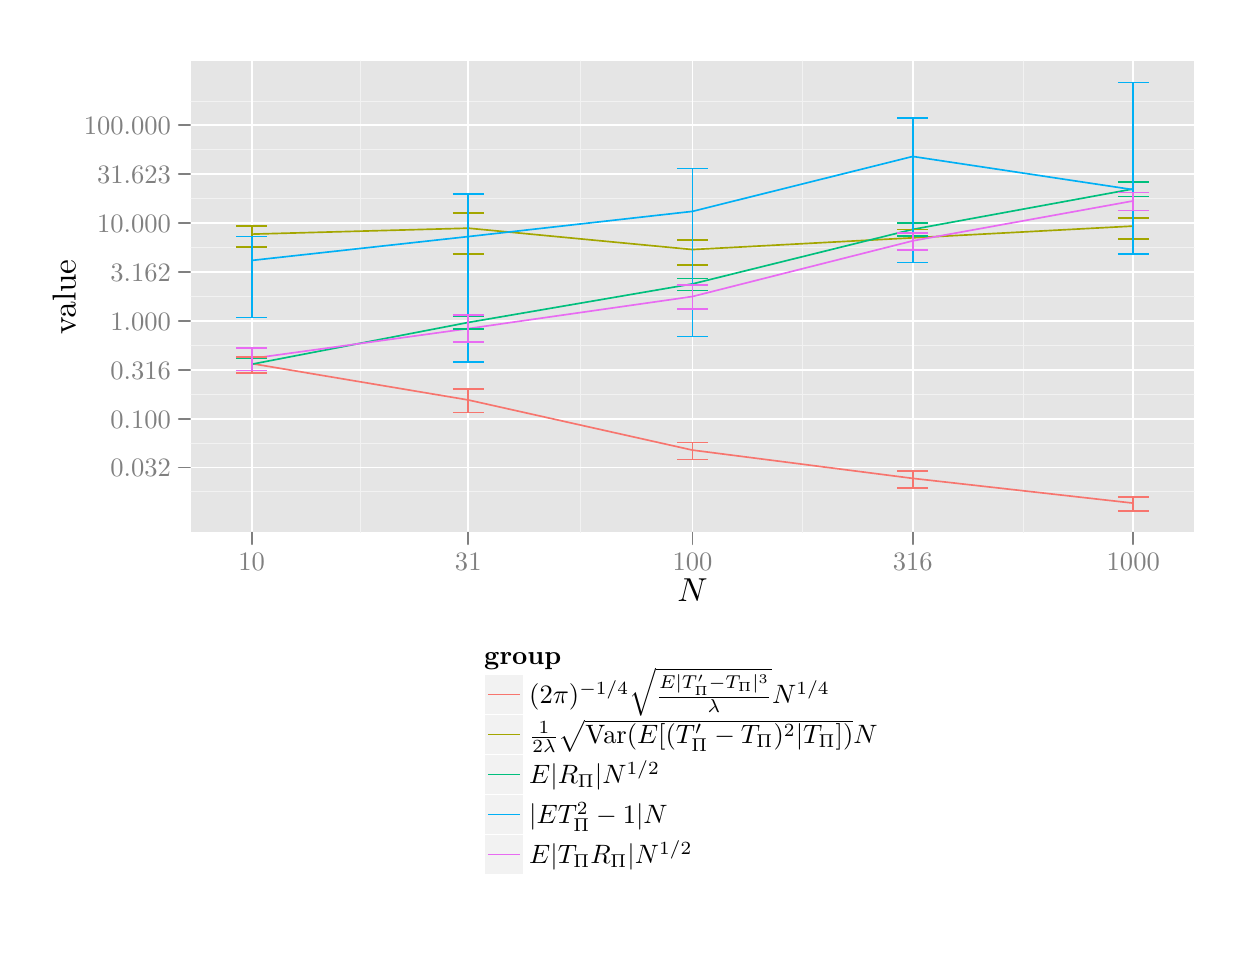
\begin{tikzpicture}[x=1pt,y=1pt]
\definecolor[named]{drawColor}{rgb}{0.00,0.00,0.00}
\definecolor[named]{fillColor}{rgb}{1.00,1.00,1.00}
\fill[color=fillColor,fill opacity=0.00,] (0,0) rectangle (433.62,325.21);
\begin{scope}
\path[clip] (  0.00,  0.00) rectangle (433.62,325.21);
\definecolor[named]{drawColor}{rgb}{0.41,0.16,0.58}
\end{scope}
\begin{scope}
\path[clip] (  0.00,  0.00) rectangle (433.62,325.21);
\definecolor[named]{drawColor}{rgb}{0.41,0.16,0.58}
\end{scope}
\begin{scope}
\path[clip] (  0.00,  0.00) rectangle (433.62,325.21);
\definecolor[named]{drawColor}{rgb}{0.41,0.16,0.58}
\end{scope}
\begin{scope}
\path[clip] (  0.00,  0.00) rectangle (433.62,325.21);
\definecolor[named]{drawColor}{rgb}{0.41,0.16,0.58}
\end{scope}
\begin{scope}
\path[clip] (  0.00,  0.00) rectangle (433.62,325.21);
\definecolor[named]{drawColor}{rgb}{0.41,0.16,0.58}
\end{scope}
\begin{scope}
\path[clip] (  0.00,  0.00) rectangle (433.62,325.21);
\definecolor[named]{drawColor}{rgb}{0.41,0.16,0.58}
\end{scope}
\begin{scope}
\path[clip] (  0.00,  0.00) rectangle (433.62,325.21);
\definecolor[named]{drawColor}{rgb}{0.41,0.16,0.58}
\end{scope}
\begin{scope}
\path[clip] (  0.00,  0.00) rectangle (433.62,325.21);
\definecolor[named]{drawColor}{rgb}{0.41,0.16,0.58}
\end{scope}
\begin{scope}
\path[clip] (  0.00,  0.00) rectangle (433.62,325.21);
\definecolor[named]{drawColor}{rgb}{0.41,0.16,0.58}
\end{scope}
\begin{scope}
\path[clip] (  0.00,  0.00) rectangle (433.62,325.21);
\definecolor[named]{drawColor}{rgb}{0.41,0.16,0.58}
\end{scope}
\begin{scope}
\path[clip] (  0.00,  0.00) rectangle (433.62,325.21);
\definecolor[named]{drawColor}{rgb}{0.41,0.16,0.58}
\end{scope}
\begin{scope}
\path[clip] (  0.00,  0.00) rectangle (433.62,325.21);
\definecolor[named]{drawColor}{rgb}{0.41,0.16,0.58}
\end{scope}
\begin{scope}
\path[clip] ( 58.88,142.81) rectangle (421.57,313.17);
\definecolor[named]{drawColor}{rgb}{0.41,0.16,0.58}
\end{scope}
\begin{scope}
\path[clip] (  0.00,  0.00) rectangle (433.62,325.21);
\definecolor[named]{drawColor}{rgb}{0.41,0.16,0.58}
\end{scope}
\begin{scope}
\path[clip] (  0.00,  0.00) rectangle (433.62,325.21);
\definecolor[named]{drawColor}{rgb}{0.41,0.16,0.58}
\end{scope}
\begin{scope}
\path[clip] (  0.00,  0.00) rectangle (433.62,325.21);
\definecolor[named]{drawColor}{rgb}{0.41,0.16,0.58}
\end{scope}
\begin{scope}
\path[clip] (  0.00,  0.00) rectangle (433.62,325.21);
\definecolor[named]{drawColor}{rgb}{0.41,0.16,0.58}
\end{scope}
\begin{scope}
\path[clip] (  0.00,  0.00) rectangle (433.62,325.21);
\definecolor[named]{drawColor}{rgb}{0.41,0.16,0.58}
\end{scope}
\begin{scope}
\path[clip] (  0.00,  0.00) rectangle (433.62,325.21);
\definecolor[named]{drawColor}{rgb}{0.41,0.16,0.58}
\end{scope}
\begin{scope}
\path[clip] (  0.00,  0.00) rectangle (433.62,325.21);
\definecolor[named]{drawColor}{rgb}{0.41,0.16,0.58}
\end{scope}
\begin{scope}
\path[clip] (  0.00,  0.00) rectangle (433.62,325.21);
\definecolor[named]{drawColor}{rgb}{0.41,0.16,0.58}
\end{scope}
\begin{scope}
\path[clip] (  0.00,  0.00) rectangle (433.62,325.21);
\definecolor[named]{drawColor}{rgb}{0.41,0.16,0.58}
\end{scope}
\begin{scope}
\path[clip] (  0.00,  0.00) rectangle (433.62,325.21);
\definecolor[named]{drawColor}{rgb}{0.41,0.16,0.58}
\end{scope}
\begin{scope}
\path[clip] (  0.00,  0.00) rectangle (433.62,325.21);
\definecolor[named]{drawColor}{rgb}{0.41,0.16,0.58}
\end{scope}
\begin{scope}
\path[clip] (  0.00,  0.00) rectangle (433.62,325.21);
\definecolor[named]{drawColor}{rgb}{0.41,0.16,0.58}
\definecolor[named]{fillColor}{rgb}{1.00,1.00,1.00}

\draw[fill=fillColor,draw opacity=0.00,] (  0.00,  0.00) rectangle (433.62,325.21);
\end{scope}
\begin{scope}
\path[clip] (  0.00,  0.00) rectangle (433.62,325.21);
\definecolor[named]{drawColor}{rgb}{0.41,0.16,0.58}
\end{scope}
\begin{scope}
\path[clip] (  0.00,  0.00) rectangle (433.62,325.21);
\definecolor[named]{drawColor}{rgb}{0.41,0.16,0.58}
\definecolor[named]{drawColor}{rgb}{0.50,0.50,0.50}

\node[color=drawColor,anchor=base east,inner sep=0pt, outer sep=0pt, scale=  0.96] at ( 51.77,162.98) {0.032};

\node[color=drawColor,anchor=base east,inner sep=0pt, outer sep=0pt, scale=  0.96] at ( 51.77,180.48) {0.100};

\node[color=drawColor,anchor=base east,inner sep=0pt, outer sep=0pt, scale=  0.96] at ( 51.77,198.16) {0.316};

\node[color=drawColor,anchor=base east,inner sep=0pt, outer sep=0pt, scale=  0.96] at ( 51.77,215.86) {1.000};

\node[color=drawColor,anchor=base east,inner sep=0pt, outer sep=0pt, scale=  0.96] at ( 51.77,233.55) {3.162};

\node[color=drawColor,anchor=base east,inner sep=0pt, outer sep=0pt, scale=  0.96] at ( 51.77,251.23) {10.000};

\node[color=drawColor,anchor=base east,inner sep=0pt, outer sep=0pt, scale=  0.96] at ( 51.77,268.92) {31.623};

\node[color=drawColor,anchor=base east,inner sep=0pt, outer sep=0pt, scale=  0.96] at ( 51.77,286.61) {100.000};
\end{scope}
\begin{scope}
\path[clip] (  0.00,  0.00) rectangle (433.62,325.21);
\definecolor[named]{drawColor}{rgb}{0.41,0.16,0.58}
\definecolor[named]{drawColor}{rgb}{0.50,0.50,0.50}

\draw[color=drawColor,line width= 0.6pt,line cap=round,line join=round,fill opacity=0.00,] ( 54.61,166.28) -- ( 58.88,166.28);

\draw[color=drawColor,line width= 0.6pt,line cap=round,line join=round,fill opacity=0.00,] ( 54.61,183.79) -- ( 58.88,183.79);

\draw[color=drawColor,line width= 0.6pt,line cap=round,line join=round,fill opacity=0.00,] ( 54.61,201.46) -- ( 58.88,201.46);

\draw[color=drawColor,line width= 0.6pt,line cap=round,line join=round,fill opacity=0.00,] ( 54.61,219.16) -- ( 58.88,219.16);

\draw[color=drawColor,line width= 0.6pt,line cap=round,line join=round,fill opacity=0.00,] ( 54.61,236.85) -- ( 58.88,236.85);

\draw[color=drawColor,line width= 0.6pt,line cap=round,line join=round,fill opacity=0.00,] ( 54.61,254.54) -- ( 58.88,254.54);

\draw[color=drawColor,line width= 0.6pt,line cap=round,line join=round,fill opacity=0.00,] ( 54.61,272.23) -- ( 58.88,272.23);

\draw[color=drawColor,line width= 0.6pt,line cap=round,line join=round,fill opacity=0.00,] ( 54.61,289.92) -- ( 58.88,289.92);
\end{scope}
\begin{scope}
\path[clip] (  0.00,  0.00) rectangle (433.62,325.21);
\definecolor[named]{drawColor}{rgb}{0.41,0.16,0.58}
\end{scope}
\begin{scope}
\path[clip] (  0.00,  0.00) rectangle (433.62,325.21);
\definecolor[named]{drawColor}{rgb}{0.41,0.16,0.58}
\end{scope}
\begin{scope}
\path[clip] (  0.00,  0.00) rectangle (433.62,325.21);
\definecolor[named]{drawColor}{rgb}{0.41,0.16,0.58}
\end{scope}
\begin{scope}
\path[clip] (  0.00,  0.00) rectangle (433.62,325.21);
\definecolor[named]{drawColor}{rgb}{0.41,0.16,0.58}
\end{scope}
\begin{scope}
\path[clip] (  0.00,  0.00) rectangle (433.62,325.21);
\definecolor[named]{drawColor}{rgb}{0.41,0.16,0.58}
\end{scope}
\begin{scope}
\path[clip] ( 58.88,142.81) rectangle (421.57,313.17);
\definecolor[named]{drawColor}{rgb}{0.41,0.16,0.58}
\definecolor[named]{fillColor}{rgb}{0.90,0.90,0.90}

\draw[fill=fillColor,draw opacity=0.00,] ( 58.88,142.81) rectangle (421.57,313.17);
\definecolor[named]{drawColor}{rgb}{0.95,0.95,0.95}

\draw[color=drawColor,line width= 0.3pt,line cap=round,line join=round,fill opacity=0.00,] ( 58.88,157.53) --
	(421.57,157.53);

\draw[color=drawColor,line width= 0.3pt,line cap=round,line join=round,fill opacity=0.00,] ( 58.88,175.03) --
	(421.57,175.03);

\draw[color=drawColor,line width= 0.3pt,line cap=round,line join=round,fill opacity=0.00,] ( 58.88,192.63) --
	(421.57,192.63);

\draw[color=drawColor,line width= 0.3pt,line cap=round,line join=round,fill opacity=0.00,] ( 58.88,210.31) --
	(421.57,210.31);

\draw[color=drawColor,line width= 0.3pt,line cap=round,line join=round,fill opacity=0.00,] ( 58.88,228.01) --
	(421.57,228.01);

\draw[color=drawColor,line width= 0.3pt,line cap=round,line join=round,fill opacity=0.00,] ( 58.88,245.70) --
	(421.57,245.70);

\draw[color=drawColor,line width= 0.3pt,line cap=round,line join=round,fill opacity=0.00,] ( 58.88,263.38) --
	(421.57,263.38);

\draw[color=drawColor,line width= 0.3pt,line cap=round,line join=round,fill opacity=0.00,] ( 58.88,281.07) --
	(421.57,281.07);

\draw[color=drawColor,line width= 0.3pt,line cap=round,line join=round,fill opacity=0.00,] ( 58.88,298.67) --
	(421.57,298.67);

\draw[color=drawColor,line width= 0.3pt,line cap=round,line join=round,fill opacity=0.00,] (120.08,142.81) --
	(120.08,313.17);

\draw[color=drawColor,line width= 0.3pt,line cap=round,line join=round,fill opacity=0.00,] (199.72,142.81) --
	(199.72,313.17);

\draw[color=drawColor,line width= 0.3pt,line cap=round,line join=round,fill opacity=0.00,] (280.02,142.81) --
	(280.02,313.17);

\draw[color=drawColor,line width= 0.3pt,line cap=round,line join=round,fill opacity=0.00,] (359.67,142.81) --
	(359.67,313.17);
\definecolor[named]{drawColor}{rgb}{1.00,1.00,1.00}

\draw[color=drawColor,line width= 0.6pt,line cap=round,line join=round,fill opacity=0.00,] ( 58.88,166.28) --
	(421.57,166.28);

\draw[color=drawColor,line width= 0.6pt,line cap=round,line join=round,fill opacity=0.00,] ( 58.88,183.79) --
	(421.57,183.79);

\draw[color=drawColor,line width= 0.6pt,line cap=round,line join=round,fill opacity=0.00,] ( 58.88,201.46) --
	(421.57,201.46);

\draw[color=drawColor,line width= 0.6pt,line cap=round,line join=round,fill opacity=0.00,] ( 58.88,219.16) --
	(421.57,219.16);

\draw[color=drawColor,line width= 0.6pt,line cap=round,line join=round,fill opacity=0.00,] ( 58.88,236.85) --
	(421.57,236.85);

\draw[color=drawColor,line width= 0.6pt,line cap=round,line join=round,fill opacity=0.00,] ( 58.88,254.54) --
	(421.57,254.54);

\draw[color=drawColor,line width= 0.6pt,line cap=round,line join=round,fill opacity=0.00,] ( 58.88,272.23) --
	(421.57,272.23);

\draw[color=drawColor,line width= 0.6pt,line cap=round,line join=round,fill opacity=0.00,] ( 58.88,289.92) --
	(421.57,289.92);

\draw[color=drawColor,line width= 0.6pt,line cap=round,line join=round,fill opacity=0.00,] ( 80.94,142.81) --
	( 80.94,313.17);

\draw[color=drawColor,line width= 0.6pt,line cap=round,line join=round,fill opacity=0.00,] (159.21,142.81) --
	(159.21,313.17);

\draw[color=drawColor,line width= 0.6pt,line cap=round,line join=round,fill opacity=0.00,] (240.23,142.81) --
	(240.23,313.17);

\draw[color=drawColor,line width= 0.6pt,line cap=round,line join=round,fill opacity=0.00,] (319.82,142.81) --
	(319.82,313.17);

\draw[color=drawColor,line width= 0.6pt,line cap=round,line join=round,fill opacity=0.00,] (399.51,142.81) --
	(399.51,313.17);
\definecolor[named]{drawColor}{rgb}{0.97,0.46,0.43}

\draw[color=drawColor,line width= 0.6pt,line join=round,fill opacity=0.00,] ( 80.94,203.83) --
	(159.21,190.68) --
	(240.23,172.56) --
	(319.82,162.35) --
	(399.51,153.40);
\definecolor[named]{drawColor}{rgb}{0.64,0.65,0.00}

\draw[color=drawColor,line width= 0.6pt,line join=round,fill opacity=0.00,] ( 80.94,250.60) --
	(159.21,252.75) --
	(240.23,245.03) --
	(319.82,249.27) --
	(399.51,253.51);
\definecolor[named]{drawColor}{rgb}{0.00,0.75,0.49}

\draw[color=drawColor,line width= 0.6pt,line join=round,fill opacity=0.00,] ( 80.94,203.59) --
	(159.21,218.69) --
	(240.23,232.62) --
	(319.82,252.32) --
	(399.51,266.94);
\definecolor[named]{drawColor}{rgb}{0.00,0.69,0.96}

\draw[color=drawColor,line width= 0.6pt,line join=round,fill opacity=0.00,] ( 80.94,241.10) --
	(159.21,249.72) --
	(240.23,258.83) --
	(319.82,278.67) --
	(399.51,266.67);
\definecolor[named]{drawColor}{rgb}{0.91,0.42,0.95}

\draw[color=drawColor,line width= 0.6pt,line join=round,fill opacity=0.00,] ( 80.94,205.66) --
	(159.21,216.47) --
	(240.23,228.06) --
	(319.82,248.18) --
	(399.51,262.61);
\definecolor[named]{drawColor}{rgb}{0.97,0.46,0.43}

\draw[color=drawColor,line width= 0.6pt,line join=round,fill opacity=0.00,] ( 75.37,206.32) --
	( 86.52,206.32);

\draw[color=drawColor,line width= 0.6pt,line join=round,fill opacity=0.00,] ( 80.94,206.32) --
	( 80.94,200.34);

\draw[color=drawColor,line width= 0.6pt,line join=round,fill opacity=0.00,] ( 75.37,200.34) --
	( 86.52,200.34);

\draw[color=drawColor,line width= 0.6pt,line join=round,fill opacity=0.00,] (153.63,194.68) --
	(164.78,194.68);

\draw[color=drawColor,line width= 0.6pt,line join=round,fill opacity=0.00,] (159.21,194.68) --
	(159.21,186.16);

\draw[color=drawColor,line width= 0.6pt,line join=round,fill opacity=0.00,] (153.63,186.16) --
	(164.78,186.16);

\draw[color=drawColor,line width= 0.6pt,line join=round,fill opacity=0.00,] (234.65,175.26) --
	(245.80,175.26);

\draw[color=drawColor,line width= 0.6pt,line join=round,fill opacity=0.00,] (240.23,175.26) --
	(240.23,169.21);

\draw[color=drawColor,line width= 0.6pt,line join=round,fill opacity=0.00,] (234.65,169.21) --
	(245.80,169.21);

\draw[color=drawColor,line width= 0.6pt,line join=round,fill opacity=0.00,] (314.25,165.12) --
	(325.40,165.12);

\draw[color=drawColor,line width= 0.6pt,line join=round,fill opacity=0.00,] (319.82,165.12) --
	(319.82,158.87);

\draw[color=drawColor,line width= 0.6pt,line join=round,fill opacity=0.00,] (314.25,158.87) --
	(325.40,158.87);

\draw[color=drawColor,line width= 0.6pt,line join=round,fill opacity=0.00,] (393.94,155.69) --
	(405.09,155.69);

\draw[color=drawColor,line width= 0.6pt,line join=round,fill opacity=0.00,] (399.51,155.69) --
	(399.51,150.56);

\draw[color=drawColor,line width= 0.6pt,line join=round,fill opacity=0.00,] (393.94,150.56) --
	(405.09,150.56);
\definecolor[named]{drawColor}{rgb}{0.64,0.65,0.00}

\draw[color=drawColor,line width= 0.6pt,line join=round,fill opacity=0.00,] ( 75.37,253.47) --
	( 86.52,253.47);

\draw[color=drawColor,line width= 0.6pt,line join=round,fill opacity=0.00,] ( 80.94,253.47) --
	( 80.94,245.96);

\draw[color=drawColor,line width= 0.6pt,line join=round,fill opacity=0.00,] ( 75.37,245.96) --
	( 86.52,245.96);

\draw[color=drawColor,line width= 0.6pt,line join=round,fill opacity=0.00,] (153.63,258.32) --
	(164.78,258.32);

\draw[color=drawColor,line width= 0.6pt,line join=round,fill opacity=0.00,] (159.21,258.32) --
	(159.21,243.44);

\draw[color=drawColor,line width= 0.6pt,line join=round,fill opacity=0.00,] (153.63,243.44) --
	(164.78,243.44);

\draw[color=drawColor,line width= 0.6pt,line join=round,fill opacity=0.00,] (234.65,248.50) --
	(245.80,248.50);

\draw[color=drawColor,line width= 0.6pt,line join=round,fill opacity=0.00,] (240.23,248.50) --
	(240.23,239.42);

\draw[color=drawColor,line width= 0.6pt,line join=round,fill opacity=0.00,] (234.65,239.42) --
	(245.80,239.42);

\draw[color=drawColor,line width= 0.6pt,line join=round,fill opacity=0.00,] (314.25,252.27) --
	(325.40,252.27);

\draw[color=drawColor,line width= 0.6pt,line join=round,fill opacity=0.00,] (319.82,252.27) --
	(319.82,244.74);

\draw[color=drawColor,line width= 0.6pt,line join=round,fill opacity=0.00,] (314.25,244.74) --
	(325.40,244.74);

\draw[color=drawColor,line width= 0.6pt,line join=round,fill opacity=0.00,] (393.94,256.44) --
	(405.09,256.44);

\draw[color=drawColor,line width= 0.6pt,line join=round,fill opacity=0.00,] (399.51,256.44) --
	(399.51,248.83);

\draw[color=drawColor,line width= 0.6pt,line join=round,fill opacity=0.00,] (393.94,248.83) --
	(405.09,248.83);
\definecolor[named]{drawColor}{rgb}{0.00,0.75,0.49}

\draw[color=drawColor,line width= 0.6pt,line join=round,fill opacity=0.00,] ( 75.37,205.70) --
	( 86.52,205.70);

\draw[color=drawColor,line width= 0.6pt,line join=round,fill opacity=0.00,] ( 80.94,205.70) --
	( 80.94,201.35);

\draw[color=drawColor,line width= 0.6pt,line join=round,fill opacity=0.00,] ( 75.37,201.35) --
	( 86.52,201.35);

\draw[color=drawColor,line width= 0.6pt,line join=round,fill opacity=0.00,] (153.63,220.88) --
	(164.78,220.88);

\draw[color=drawColor,line width= 0.6pt,line join=round,fill opacity=0.00,] (159.21,220.88) --
	(159.21,216.35);

\draw[color=drawColor,line width= 0.6pt,line join=round,fill opacity=0.00,] (153.63,216.35) --
	(164.78,216.35);

\draw[color=drawColor,line width= 0.6pt,line join=round,fill opacity=0.00,] (234.65,234.62) --
	(245.80,234.62);

\draw[color=drawColor,line width= 0.6pt,line join=round,fill opacity=0.00,] (240.23,234.62) --
	(240.23,230.23);

\draw[color=drawColor,line width= 0.6pt,line join=round,fill opacity=0.00,] (234.65,230.23) --
	(245.80,230.23);

\draw[color=drawColor,line width= 0.6pt,line join=round,fill opacity=0.00,] (314.25,254.55) --
	(325.40,254.55);

\draw[color=drawColor,line width= 0.6pt,line join=round,fill opacity=0.00,] (319.82,254.55) --
	(319.82,249.92);

\draw[color=drawColor,line width= 0.6pt,line join=round,fill opacity=0.00,] (314.25,249.92) --
	(325.40,249.92);

\draw[color=drawColor,line width= 0.6pt,line join=round,fill opacity=0.00,] (393.94,269.37) --
	(405.09,269.37);

\draw[color=drawColor,line width= 0.6pt,line join=round,fill opacity=0.00,] (399.51,269.37) --
	(399.51,264.26);

\draw[color=drawColor,line width= 0.6pt,line join=round,fill opacity=0.00,] (393.94,264.26) --
	(405.09,264.26);
\definecolor[named]{drawColor}{rgb}{0.00,0.69,0.96}

\draw[color=drawColor,line width= 0.6pt,line join=round,fill opacity=0.00,] ( 75.37,249.80) --
	( 86.52,249.80);

\draw[color=drawColor,line width= 0.6pt,line join=round,fill opacity=0.00,] ( 80.94,249.80) --
	( 80.94,220.53);

\draw[color=drawColor,line width= 0.6pt,line join=round,fill opacity=0.00,] ( 75.37,220.53) --
	( 86.52,220.53);

\draw[color=drawColor,line width= 0.6pt,line join=round,fill opacity=0.00,] (153.63,265.15) --
	(164.78,265.15);

\draw[color=drawColor,line width= 0.6pt,line join=round,fill opacity=0.00,] (159.21,265.15) --
	(159.21,204.45);

\draw[color=drawColor,line width= 0.6pt,line join=round,fill opacity=0.00,] (153.63,204.45) --
	(164.78,204.45);

\draw[color=drawColor,line width= 0.6pt,line join=round,fill opacity=0.00,] (234.65,274.32) --
	(245.80,274.32);

\draw[color=drawColor,line width= 0.6pt,line join=round,fill opacity=0.00,] (240.23,274.32) --
	(240.23,213.60);

\draw[color=drawColor,line width= 0.6pt,line join=round,fill opacity=0.00,] (234.65,213.60) --
	(245.80,213.60);

\draw[color=drawColor,line width= 0.6pt,line join=round,fill opacity=0.00,] (314.25,292.55) --
	(325.40,292.55);

\draw[color=drawColor,line width= 0.6pt,line join=round,fill opacity=0.00,] (319.82,292.55) --
	(319.82,240.36);

\draw[color=drawColor,line width= 0.6pt,line join=round,fill opacity=0.00,] (314.25,240.36) --
	(325.40,240.36);

\draw[color=drawColor,line width= 0.6pt,line join=round,fill opacity=0.00,] (393.94,305.43) --
	(405.09,305.43);

\draw[color=drawColor,line width= 0.6pt,line join=round,fill opacity=0.00,] (399.51,305.43) --
	(399.51,243.53);

\draw[color=drawColor,line width= 0.6pt,line join=round,fill opacity=0.00,] (393.94,243.53) --
	(405.09,243.53);
\definecolor[named]{drawColor}{rgb}{0.91,0.42,0.95}

\draw[color=drawColor,line width= 0.6pt,line join=round,fill opacity=0.00,] ( 75.37,209.42) --
	( 86.52,209.42);

\draw[color=drawColor,line width= 0.6pt,line join=round,fill opacity=0.00,] ( 80.94,209.42) --
	( 80.94,201.38);

\draw[color=drawColor,line width= 0.6pt,line join=round,fill opacity=0.00,] ( 75.37,201.38) --
	( 86.52,201.38);

\draw[color=drawColor,line width= 0.6pt,line join=round,fill opacity=0.00,] (153.63,221.29) --
	(164.78,221.29);

\draw[color=drawColor,line width= 0.6pt,line join=round,fill opacity=0.00,] (159.21,221.29) --
	(159.21,211.56);

\draw[color=drawColor,line width= 0.6pt,line join=round,fill opacity=0.00,] (153.63,211.56) --
	(164.78,211.56);

\draw[color=drawColor,line width= 0.6pt,line join=round,fill opacity=0.00,] (234.65,232.16) --
	(245.80,232.16);

\draw[color=drawColor,line width= 0.6pt,line join=round,fill opacity=0.00,] (240.23,232.16) --
	(240.23,223.62);

\draw[color=drawColor,line width= 0.6pt,line join=round,fill opacity=0.00,] (234.65,223.62) --
	(245.80,223.62);

\draw[color=drawColor,line width= 0.6pt,line join=round,fill opacity=0.00,] (314.25,251.01) --
	(325.40,251.01);

\draw[color=drawColor,line width= 0.6pt,line join=round,fill opacity=0.00,] (319.82,251.01) --
	(319.82,244.79);

\draw[color=drawColor,line width= 0.6pt,line join=round,fill opacity=0.00,] (314.25,244.79) --
	(325.40,244.79);

\draw[color=drawColor,line width= 0.6pt,line join=round,fill opacity=0.00,] (393.94,265.59) --
	(405.09,265.59);

\draw[color=drawColor,line width= 0.6pt,line join=round,fill opacity=0.00,] (399.51,265.59) --
	(399.51,259.13);

\draw[color=drawColor,line width= 0.6pt,line join=round,fill opacity=0.00,] (393.94,259.13) --
	(405.09,259.13);
\end{scope}
\begin{scope}
\path[clip] (  0.00,  0.00) rectangle (433.62,325.21);
\definecolor[named]{drawColor}{rgb}{0.41,0.16,0.58}
\end{scope}
\begin{scope}
\path[clip] (  0.00,  0.00) rectangle (433.62,325.21);
\definecolor[named]{drawColor}{rgb}{0.41,0.16,0.58}
\definecolor[named]{drawColor}{rgb}{0.50,0.50,0.50}

\node[color=drawColor,anchor=base,inner sep=0pt, outer sep=0pt, scale=  0.96] at ( 80.94,129.09) {10};

\node[color=drawColor,anchor=base,inner sep=0pt, outer sep=0pt, scale=  0.96] at (159.21,129.09) {31};

\node[color=drawColor,anchor=base,inner sep=0pt, outer sep=0pt, scale=  0.96] at (240.23,129.09) {100};

\node[color=drawColor,anchor=base,inner sep=0pt, outer sep=0pt, scale=  0.96] at (319.82,129.09) {316};

\node[color=drawColor,anchor=base,inner sep=0pt, outer sep=0pt, scale=  0.96] at (399.51,129.09) {1000};
\end{scope}
\begin{scope}
\path[clip] (  0.00,  0.00) rectangle (433.62,325.21);
\definecolor[named]{drawColor}{rgb}{0.41,0.16,0.58}
\definecolor[named]{drawColor}{rgb}{0.50,0.50,0.50}

\draw[color=drawColor,line width= 0.6pt,line cap=round,line join=round,fill opacity=0.00,] ( 80.94,138.55) -- ( 80.94,142.81);

\draw[color=drawColor,line width= 0.6pt,line cap=round,line join=round,fill opacity=0.00,] (159.21,138.55) -- (159.21,142.81);

\draw[color=drawColor,line width= 0.6pt,line cap=round,line join=round,fill opacity=0.00,] (240.23,138.55) -- (240.23,142.81);

\draw[color=drawColor,line width= 0.6pt,line cap=round,line join=round,fill opacity=0.00,] (319.82,138.55) -- (319.82,142.81);

\draw[color=drawColor,line width= 0.6pt,line cap=round,line join=round,fill opacity=0.00,] (399.51,138.55) -- (399.51,142.81);
\end{scope}
\begin{scope}
\path[clip] (  0.00,  0.00) rectangle (433.62,325.21);
\definecolor[named]{drawColor}{rgb}{0.41,0.16,0.58}
\end{scope}
\begin{scope}
\path[clip] (  0.00,  0.00) rectangle (433.62,325.21);
\definecolor[named]{drawColor}{rgb}{0.41,0.16,0.58}
\end{scope}
\begin{scope}
\path[clip] (  0.00,  0.00) rectangle (433.62,325.21);
\definecolor[named]{drawColor}{rgb}{0.41,0.16,0.58}
\end{scope}
\begin{scope}
\path[clip] (  0.00,  0.00) rectangle (433.62,325.21);
\definecolor[named]{drawColor}{rgb}{0.41,0.16,0.58}
\end{scope}
\begin{scope}
\path[clip] (  0.00,  0.00) rectangle (433.62,325.21);
\definecolor[named]{drawColor}{rgb}{0.41,0.16,0.58}
\end{scope}
\begin{scope}
\path[clip] (  0.00,  0.00) rectangle (433.62,325.21);
\definecolor[named]{drawColor}{rgb}{0.41,0.16,0.58}
\definecolor[named]{drawColor}{rgb}{0.00,0.00,0.00}

\node[color=drawColor,anchor=base,inner sep=0pt, outer sep=0pt, scale=  1.20] at (240.23,117.81) {$N$};
\end{scope}
\begin{scope}
\path[clip] (  0.00,  0.00) rectangle (433.62,325.21);
\definecolor[named]{drawColor}{rgb}{0.41,0.16,0.58}
\end{scope}
\begin{scope}
\path[clip] (  0.00,  0.00) rectangle (433.62,325.21);
\definecolor[named]{drawColor}{rgb}{0.41,0.16,0.58}
\definecolor[named]{drawColor}{rgb}{0.00,0.00,0.00}

\node[rotate= 90.00,color=drawColor,anchor=base,inner sep=0pt, outer sep=0pt, scale=  1.20] at ( 17.30,227.99) {value};
\end{scope}
\begin{scope}
\path[clip] (  0.00,  0.00) rectangle (433.62,325.21);
\definecolor[named]{drawColor}{rgb}{0.41,0.16,0.58}
\end{scope}
\begin{scope}
\path[clip] (  0.00,  0.00) rectangle (433.62,325.21);
\definecolor[named]{drawColor}{rgb}{0.41,0.16,0.58}
\end{scope}
\begin{scope}
\path[clip] (  0.00,  0.00) rectangle (433.62,325.21);
\definecolor[named]{drawColor}{rgb}{0.41,0.16,0.58}
\end{scope}
\begin{scope}
\path[clip] (  0.00,  0.00) rectangle (433.62,325.21);
\definecolor[named]{drawColor}{rgb}{0.41,0.16,0.58}
\end{scope}
\begin{scope}
\path[clip] (  0.00,  0.00) rectangle (433.62,325.21);
\definecolor[named]{drawColor}{rgb}{0.41,0.16,0.58}
\end{scope}
\begin{scope}
\path[clip] (  0.00,  0.00) rectangle (433.62,325.21);
\definecolor[named]{drawColor}{rgb}{0.41,0.16,0.58}
\end{scope}
\begin{scope}
\path[clip] (  0.00,  0.00) rectangle (433.62,325.21);
\definecolor[named]{drawColor}{rgb}{0.41,0.16,0.58}
\end{scope}
\begin{scope}
\path[clip] (  0.00,  0.00) rectangle (433.62,325.21);
\definecolor[named]{drawColor}{rgb}{0.41,0.16,0.58}
\end{scope}
\begin{scope}
\path[clip] (  0.00,  0.00) rectangle (433.62,325.21);
\definecolor[named]{drawColor}{rgb}{0.41,0.16,0.58}
\end{scope}
\begin{scope}
\path[clip] (  0.00,  0.00) rectangle (433.62,325.21);
\definecolor[named]{drawColor}{rgb}{0.41,0.16,0.58}
\end{scope}
\begin{scope}
\path[clip] (  0.00,  0.00) rectangle (433.62,325.21);
\definecolor[named]{drawColor}{rgb}{0.41,0.16,0.58}
\end{scope}
\begin{scope}
\path[clip] (  0.00,  0.00) rectangle (433.62,325.21);
\definecolor[named]{drawColor}{rgb}{0.41,0.16,0.58}
\end{scope}
\begin{scope}
\path[clip] (  0.00,  0.00) rectangle (433.62,325.21);
\definecolor[named]{drawColor}{rgb}{0.41,0.16,0.58}
\end{scope}
\begin{scope}
\path[clip] (  0.00,  0.00) rectangle (433.62,325.21);
\definecolor[named]{drawColor}{rgb}{0.41,0.16,0.58}
\end{scope}
\begin{scope}
\path[clip] (  0.00,  0.00) rectangle (433.62,325.21);
\definecolor[named]{drawColor}{rgb}{0.41,0.16,0.58}
\end{scope}
\begin{scope}
\path[clip] (  0.00,  0.00) rectangle (433.62,325.21);
\definecolor[named]{drawColor}{rgb}{0.41,0.16,0.58}
\end{scope}
\begin{scope}
\path[clip] (  0.00,  0.00) rectangle (433.62,325.21);
\definecolor[named]{drawColor}{rgb}{0.41,0.16,0.58}
\end{scope}
\begin{scope}
\path[clip] (  0.00,  0.00) rectangle (433.62,325.21);
\definecolor[named]{drawColor}{rgb}{0.41,0.16,0.58}
\end{scope}
\begin{scope}
\path[clip] (  0.00,  0.00) rectangle (433.62,325.21);
\definecolor[named]{drawColor}{rgb}{0.41,0.16,0.58}
\end{scope}
\begin{scope}
\path[clip] (  0.00,  0.00) rectangle (433.62,325.21);
\definecolor[named]{drawColor}{rgb}{0.41,0.16,0.58}
\end{scope}
\begin{scope}
\path[clip] (  0.00,  0.00) rectangle (433.62,325.21);
\definecolor[named]{drawColor}{rgb}{0.41,0.16,0.58}
\end{scope}
\begin{scope}
\path[clip] (  0.00,  0.00) rectangle (433.62,325.21);
\definecolor[named]{drawColor}{rgb}{0.41,0.16,0.58}
\end{scope}
\begin{scope}
\path[clip] (  0.00,  0.00) rectangle (433.62,325.21);
\definecolor[named]{drawColor}{rgb}{0.41,0.16,0.58}
\end{scope}
\begin{scope}
\path[clip] (  0.00,  0.00) rectangle (433.62,325.21);
\definecolor[named]{drawColor}{rgb}{0.41,0.16,0.58}
\end{scope}
\begin{scope}
\path[clip] (  0.00,  0.00) rectangle (433.62,325.21);
\definecolor[named]{drawColor}{rgb}{0.41,0.16,0.58}
\definecolor[named]{drawColor}{rgb}{1.00,1.00,1.00}

\draw[color=drawColor,line width= 0.6pt,line cap=round,line join=round,fill opacity=0.00,] (160.71, 14.89) rectangle (319.75,105.93);
\end{scope}
\begin{scope}
\path[clip] (  0.00,  0.00) rectangle (433.62,325.21);
\definecolor[named]{drawColor}{rgb}{0.41,0.16,0.58}
\definecolor[named]{drawColor}{rgb}{0.00,0.00,0.00}

\node[color=drawColor,anchor=base west,inner sep=0pt, outer sep=0pt, scale=  0.96] at (164.98, 95.04) {\bfseries group};
\end{scope}
\begin{scope}
\path[clip] (  0.00,  0.00) rectangle (433.62,325.21);
\definecolor[named]{drawColor}{rgb}{0.41,0.16,0.58}
\definecolor[named]{drawColor}{rgb}{1.00,1.00,1.00}
\definecolor[named]{fillColor}{rgb}{0.95,0.95,0.95}

\draw[color=drawColor,line width= 0.6pt,line cap=round,line join=round,fill=fillColor,] (164.98, 76.97) rectangle (179.43, 91.43);
\end{scope}
\begin{scope}
\path[clip] (  0.00,  0.00) rectangle (433.62,325.21);
\definecolor[named]{drawColor}{rgb}{0.41,0.16,0.58}
\definecolor[named]{drawColor}{rgb}{0.97,0.46,0.43}

\draw[color=drawColor,line width= 0.6pt,line join=round,fill opacity=0.00,] (166.42, 84.20) -- (177.98, 84.20);
\end{scope}
\begin{scope}
\path[clip] (  0.00,  0.00) rectangle (433.62,325.21);
\definecolor[named]{drawColor}{rgb}{0.41,0.16,0.58}
\definecolor[named]{drawColor}{rgb}{0.97,0.46,0.43}

\draw[color=drawColor,line width= 0.6pt,line join=round,fill opacity=0.00,] (166.42, 84.20) -- (177.98, 84.20);
\end{scope}
\begin{scope}
\path[clip] (  0.00,  0.00) rectangle (433.62,325.21);
\definecolor[named]{drawColor}{rgb}{0.41,0.16,0.58}
\definecolor[named]{drawColor}{rgb}{1.00,1.00,1.00}
\definecolor[named]{fillColor}{rgb}{0.95,0.95,0.95}

\draw[color=drawColor,line width= 0.6pt,line cap=round,line join=round,fill=fillColor,] (164.98, 62.52) rectangle (179.43, 76.97);
\end{scope}
\begin{scope}
\path[clip] (  0.00,  0.00) rectangle (433.62,325.21);
\definecolor[named]{drawColor}{rgb}{0.41,0.16,0.58}
\definecolor[named]{drawColor}{rgb}{0.64,0.65,0.00}

\draw[color=drawColor,line width= 0.6pt,line join=round,fill opacity=0.00,] (166.42, 69.75) -- (177.98, 69.75);
\end{scope}
\begin{scope}
\path[clip] (  0.00,  0.00) rectangle (433.62,325.21);
\definecolor[named]{drawColor}{rgb}{0.41,0.16,0.58}
\definecolor[named]{drawColor}{rgb}{0.64,0.65,0.00}

\draw[color=drawColor,line width= 0.6pt,line join=round,fill opacity=0.00,] (166.42, 69.75) -- (177.98, 69.75);
\end{scope}
\begin{scope}
\path[clip] (  0.00,  0.00) rectangle (433.62,325.21);
\definecolor[named]{drawColor}{rgb}{0.41,0.16,0.58}
\definecolor[named]{drawColor}{rgb}{1.00,1.00,1.00}
\definecolor[named]{fillColor}{rgb}{0.95,0.95,0.95}

\draw[color=drawColor,line width= 0.6pt,line cap=round,line join=round,fill=fillColor,] (164.98, 48.07) rectangle (179.43, 62.52);
\end{scope}
\begin{scope}
\path[clip] (  0.00,  0.00) rectangle (433.62,325.21);
\definecolor[named]{drawColor}{rgb}{0.41,0.16,0.58}
\definecolor[named]{drawColor}{rgb}{0.00,0.75,0.49}

\draw[color=drawColor,line width= 0.6pt,line join=round,fill opacity=0.00,] (166.42, 55.29) -- (177.98, 55.29);
\end{scope}
\begin{scope}
\path[clip] (  0.00,  0.00) rectangle (433.62,325.21);
\definecolor[named]{drawColor}{rgb}{0.41,0.16,0.58}
\definecolor[named]{drawColor}{rgb}{0.00,0.75,0.49}

\draw[color=drawColor,line width= 0.6pt,line join=round,fill opacity=0.00,] (166.42, 55.29) -- (177.98, 55.29);
\end{scope}
\begin{scope}
\path[clip] (  0.00,  0.00) rectangle (433.62,325.21);
\definecolor[named]{drawColor}{rgb}{0.41,0.16,0.58}
\definecolor[named]{drawColor}{rgb}{1.00,1.00,1.00}
\definecolor[named]{fillColor}{rgb}{0.95,0.95,0.95}

\draw[color=drawColor,line width= 0.6pt,line cap=round,line join=round,fill=fillColor,] (164.98, 33.61) rectangle (179.43, 48.07);
\end{scope}
\begin{scope}
\path[clip] (  0.00,  0.00) rectangle (433.62,325.21);
\definecolor[named]{drawColor}{rgb}{0.41,0.16,0.58}
\definecolor[named]{drawColor}{rgb}{0.00,0.69,0.96}

\draw[color=drawColor,line width= 0.6pt,line join=round,fill opacity=0.00,] (166.42, 40.84) -- (177.98, 40.84);
\end{scope}
\begin{scope}
\path[clip] (  0.00,  0.00) rectangle (433.62,325.21);
\definecolor[named]{drawColor}{rgb}{0.41,0.16,0.58}
\definecolor[named]{drawColor}{rgb}{0.00,0.69,0.96}

\draw[color=drawColor,line width= 0.6pt,line join=round,fill opacity=0.00,] (166.42, 40.84) -- (177.98, 40.84);
\end{scope}
\begin{scope}
\path[clip] (  0.00,  0.00) rectangle (433.62,325.21);
\definecolor[named]{drawColor}{rgb}{0.41,0.16,0.58}
\definecolor[named]{drawColor}{rgb}{1.00,1.00,1.00}
\definecolor[named]{fillColor}{rgb}{0.95,0.95,0.95}

\draw[color=drawColor,line width= 0.6pt,line cap=round,line join=round,fill=fillColor,] (164.98, 19.16) rectangle (179.43, 33.61);
\end{scope}
\begin{scope}
\path[clip] (  0.00,  0.00) rectangle (433.62,325.21);
\definecolor[named]{drawColor}{rgb}{0.41,0.16,0.58}
\definecolor[named]{drawColor}{rgb}{0.91,0.42,0.95}

\draw[color=drawColor,line width= 0.6pt,line join=round,fill opacity=0.00,] (166.42, 26.39) -- (177.98, 26.39);
\end{scope}
\begin{scope}
\path[clip] (  0.00,  0.00) rectangle (433.62,325.21);
\definecolor[named]{drawColor}{rgb}{0.41,0.16,0.58}
\definecolor[named]{drawColor}{rgb}{0.91,0.42,0.95}

\draw[color=drawColor,line width= 0.6pt,line join=round,fill opacity=0.00,] (166.42, 26.39) -- (177.98, 26.39);
\end{scope}
\begin{scope}
\path[clip] (  0.00,  0.00) rectangle (433.62,325.21);
\definecolor[named]{drawColor}{rgb}{0.41,0.16,0.58}
\definecolor[named]{drawColor}{rgb}{0.00,0.00,0.00}

\node[color=drawColor,anchor=base west,inner sep=0pt, outer sep=0pt, scale=  0.96] at (181.24, 80.90) {$(2\pi)^{-1/4}\sqrt{\frac{\mathbb{E}|T'_{\Pi}-T_{\Pi}|^3}{\lambda}}N^{1/4}\quad $};
\end{scope}
\begin{scope}
\path[clip] (  0.00,  0.00) rectangle (433.62,325.21);
\definecolor[named]{drawColor}{rgb}{0.41,0.16,0.58}
\definecolor[named]{drawColor}{rgb}{0.00,0.00,0.00}

\node[color=drawColor,anchor=base west,inner sep=0pt, outer sep=0pt, scale=  0.96] at (181.24, 66.44) {$\frac{1}{2\lambda}\sqrt{\mathrm{Var}(\mathbb{E}[(T'_{\Pi}-T_{\Pi})^2|T_{\Pi}])}N\quad $};
\end{scope}
\begin{scope}
\path[clip] (  0.00,  0.00) rectangle (433.62,325.21);
\definecolor[named]{drawColor}{rgb}{0.41,0.16,0.58}
\definecolor[named]{drawColor}{rgb}{0.00,0.00,0.00}

\node[color=drawColor,anchor=base west,inner sep=0pt, outer sep=0pt, scale=  0.96] at (181.24, 51.99) {$\mathbb{E}|R_{\Pi}|N^{1/2}\quad $};
\end{scope}
\begin{scope}
\path[clip] (  0.00,  0.00) rectangle (433.62,325.21);
\definecolor[named]{drawColor}{rgb}{0.41,0.16,0.58}
\definecolor[named]{drawColor}{rgb}{0.00,0.00,0.00}

\node[color=drawColor,anchor=base west,inner sep=0pt, outer sep=0pt, scale=  0.96] at (181.24, 37.53) {$|\mathbb{E}T_{\Pi}^2-1|N\quad $};
\end{scope}
\begin{scope}
\path[clip] (  0.00,  0.00) rectangle (433.62,325.21);
\definecolor[named]{drawColor}{rgb}{0.41,0.16,0.58}
\definecolor[named]{drawColor}{rgb}{0.00,0.00,0.00}

\node[color=drawColor,anchor=base west,inner sep=0pt, outer sep=0pt, scale=  0.96] at (181.24, 23.08) {$\mathbb{E}|T_{\Pi}R_{\Pi}|N^{1/2}\quad $};
\end{scope}
\begin{scope}
\path[clip] (  0.00,  0.00) rectangle (433.62,325.21);
\definecolor[named]{drawColor}{rgb}{0.41,0.16,0.58}
\end{scope}
\begin{scope}
\path[clip] (  0.00,  0.00) rectangle (433.62,325.21);
\definecolor[named]{drawColor}{rgb}{0.41,0.16,0.58}
\end{scope}
\begin{scope}
\path[clip] (  0.00,  0.00) rectangle (433.62,325.21);
\definecolor[named]{drawColor}{rgb}{0.41,0.16,0.58}
\end{scope}
\end{tikzpicture}

  \caption{Log-log plot of values for each term in the bound, simulating the conditional expectation
    by Monte Carlo (1,000 MC draws, 100 permutations each).}
\end{figure}
The MC error is too large, and we see some scaled bounds actually increase.
\clearpage

\subsection{Exact Conditional Expectation Calculations}
Here we $T'$ for all $N^2$ group-switching transpositions $(I, J)$:
\begin{figure}[!ht]
  \centering
  % Created by tikzDevice version 0.6.2 on 2012-04-24 08:02:18
% !TEX encoding = UTF-8 Unicode
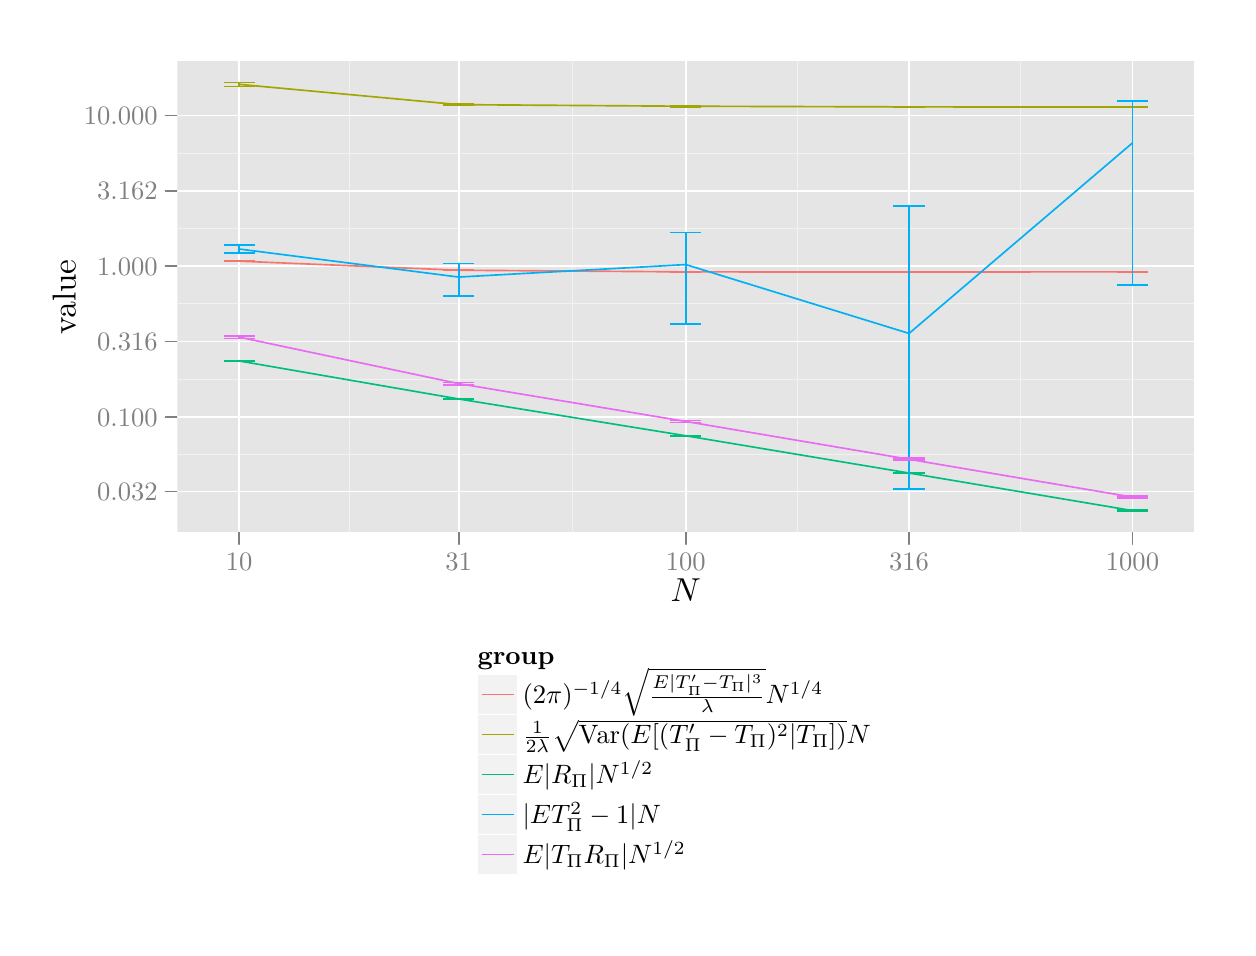
\begin{tikzpicture}[x=1pt,y=1pt]
\definecolor[named]{drawColor}{rgb}{0.00,0.00,0.00}
\definecolor[named]{fillColor}{rgb}{1.00,1.00,1.00}
\fill[color=fillColor,fill opacity=0.00,] (0,0) rectangle (433.62,325.21);
\begin{scope}
\path[clip] (  0.00,  0.00) rectangle (433.62,325.21);
\definecolor[named]{drawColor}{rgb}{0.41,0.16,0.58}
\end{scope}
\begin{scope}
\path[clip] (  0.00,  0.00) rectangle (433.62,325.21);
\definecolor[named]{drawColor}{rgb}{0.41,0.16,0.58}
\end{scope}
\begin{scope}
\path[clip] (  0.00,  0.00) rectangle (433.62,325.21);
\definecolor[named]{drawColor}{rgb}{0.41,0.16,0.58}
\end{scope}
\begin{scope}
\path[clip] (  0.00,  0.00) rectangle (433.62,325.21);
\definecolor[named]{drawColor}{rgb}{0.41,0.16,0.58}
\end{scope}
\begin{scope}
\path[clip] (  0.00,  0.00) rectangle (433.62,325.21);
\definecolor[named]{drawColor}{rgb}{0.41,0.16,0.58}
\end{scope}
\begin{scope}
\path[clip] (  0.00,  0.00) rectangle (433.62,325.21);
\definecolor[named]{drawColor}{rgb}{0.41,0.16,0.58}
\end{scope}
\begin{scope}
\path[clip] (  0.00,  0.00) rectangle (433.62,325.21);
\definecolor[named]{drawColor}{rgb}{0.41,0.16,0.58}
\end{scope}
\begin{scope}
\path[clip] (  0.00,  0.00) rectangle (433.62,325.21);
\definecolor[named]{drawColor}{rgb}{0.41,0.16,0.58}
\end{scope}
\begin{scope}
\path[clip] (  0.00,  0.00) rectangle (433.62,325.21);
\definecolor[named]{drawColor}{rgb}{0.41,0.16,0.58}
\end{scope}
\begin{scope}
\path[clip] (  0.00,  0.00) rectangle (433.62,325.21);
\definecolor[named]{drawColor}{rgb}{0.41,0.16,0.58}
\end{scope}
\begin{scope}
\path[clip] (  0.00,  0.00) rectangle (433.62,325.21);
\definecolor[named]{drawColor}{rgb}{0.41,0.16,0.58}
\end{scope}
\begin{scope}
\path[clip] (  0.00,  0.00) rectangle (433.62,325.21);
\definecolor[named]{drawColor}{rgb}{0.41,0.16,0.58}
\end{scope}
\begin{scope}
\path[clip] ( 54.08,142.81) rectangle (421.57,313.17);
\definecolor[named]{drawColor}{rgb}{0.41,0.16,0.58}
\end{scope}
\begin{scope}
\path[clip] (  0.00,  0.00) rectangle (433.62,325.21);
\definecolor[named]{drawColor}{rgb}{0.41,0.16,0.58}
\end{scope}
\begin{scope}
\path[clip] (  0.00,  0.00) rectangle (433.62,325.21);
\definecolor[named]{drawColor}{rgb}{0.41,0.16,0.58}
\end{scope}
\begin{scope}
\path[clip] (  0.00,  0.00) rectangle (433.62,325.21);
\definecolor[named]{drawColor}{rgb}{0.41,0.16,0.58}
\end{scope}
\begin{scope}
\path[clip] (  0.00,  0.00) rectangle (433.62,325.21);
\definecolor[named]{drawColor}{rgb}{0.41,0.16,0.58}
\end{scope}
\begin{scope}
\path[clip] (  0.00,  0.00) rectangle (433.62,325.21);
\definecolor[named]{drawColor}{rgb}{0.41,0.16,0.58}
\end{scope}
\begin{scope}
\path[clip] (  0.00,  0.00) rectangle (433.62,325.21);
\definecolor[named]{drawColor}{rgb}{0.41,0.16,0.58}
\end{scope}
\begin{scope}
\path[clip] (  0.00,  0.00) rectangle (433.62,325.21);
\definecolor[named]{drawColor}{rgb}{0.41,0.16,0.58}
\end{scope}
\begin{scope}
\path[clip] (  0.00,  0.00) rectangle (433.62,325.21);
\definecolor[named]{drawColor}{rgb}{0.41,0.16,0.58}
\end{scope}
\begin{scope}
\path[clip] (  0.00,  0.00) rectangle (433.62,325.21);
\definecolor[named]{drawColor}{rgb}{0.41,0.16,0.58}
\end{scope}
\begin{scope}
\path[clip] (  0.00,  0.00) rectangle (433.62,325.21);
\definecolor[named]{drawColor}{rgb}{0.41,0.16,0.58}
\end{scope}
\begin{scope}
\path[clip] (  0.00,  0.00) rectangle (433.62,325.21);
\definecolor[named]{drawColor}{rgb}{0.41,0.16,0.58}
\end{scope}
\begin{scope}
\path[clip] (  0.00,  0.00) rectangle (433.62,325.21);
\definecolor[named]{drawColor}{rgb}{0.41,0.16,0.58}
\definecolor[named]{fillColor}{rgb}{1.00,1.00,1.00}

\draw[fill=fillColor,draw opacity=0.00,] (  0.00,  0.00) rectangle (433.62,325.21);
\end{scope}
\begin{scope}
\path[clip] (  0.00,  0.00) rectangle (433.62,325.21);
\definecolor[named]{drawColor}{rgb}{0.41,0.16,0.58}
\end{scope}
\begin{scope}
\path[clip] (  0.00,  0.00) rectangle (433.62,325.21);
\definecolor[named]{drawColor}{rgb}{0.41,0.16,0.58}
\definecolor[named]{drawColor}{rgb}{0.50,0.50,0.50}

\node[color=drawColor,anchor=base east,inner sep=0pt, outer sep=0pt, scale=  0.96] at ( 46.97,154.31) {0.032};

\node[color=drawColor,anchor=base east,inner sep=0pt, outer sep=0pt, scale=  0.96] at ( 46.97,181.26) {0.100};

\node[color=drawColor,anchor=base east,inner sep=0pt, outer sep=0pt, scale=  0.96] at ( 46.97,208.47) {0.316};

\node[color=drawColor,anchor=base east,inner sep=0pt, outer sep=0pt, scale=  0.96] at ( 46.97,235.72) {1.000};

\node[color=drawColor,anchor=base east,inner sep=0pt, outer sep=0pt, scale=  0.96] at ( 46.97,262.94) {3.162};

\node[color=drawColor,anchor=base east,inner sep=0pt, outer sep=0pt, scale=  0.96] at ( 46.97,290.17) {10.000};
\end{scope}
\begin{scope}
\path[clip] (  0.00,  0.00) rectangle (433.62,325.21);
\definecolor[named]{drawColor}{rgb}{0.41,0.16,0.58}
\definecolor[named]{drawColor}{rgb}{0.50,0.50,0.50}

\draw[color=drawColor,line width= 0.6pt,line cap=round,line join=round,fill opacity=0.00,] ( 49.82,157.62) -- ( 54.08,157.62);

\draw[color=drawColor,line width= 0.6pt,line cap=round,line join=round,fill opacity=0.00,] ( 49.82,184.56) -- ( 54.08,184.56);

\draw[color=drawColor,line width= 0.6pt,line cap=round,line join=round,fill opacity=0.00,] ( 49.82,211.78) -- ( 54.08,211.78);

\draw[color=drawColor,line width= 0.6pt,line cap=round,line join=round,fill opacity=0.00,] ( 49.82,239.02) -- ( 54.08,239.02);

\draw[color=drawColor,line width= 0.6pt,line cap=round,line join=round,fill opacity=0.00,] ( 49.82,266.25) -- ( 54.08,266.25);

\draw[color=drawColor,line width= 0.6pt,line cap=round,line join=round,fill opacity=0.00,] ( 49.82,293.48) -- ( 54.08,293.48);
\end{scope}
\begin{scope}
\path[clip] (  0.00,  0.00) rectangle (433.62,325.21);
\definecolor[named]{drawColor}{rgb}{0.41,0.16,0.58}
\end{scope}
\begin{scope}
\path[clip] (  0.00,  0.00) rectangle (433.62,325.21);
\definecolor[named]{drawColor}{rgb}{0.41,0.16,0.58}
\end{scope}
\begin{scope}
\path[clip] (  0.00,  0.00) rectangle (433.62,325.21);
\definecolor[named]{drawColor}{rgb}{0.41,0.16,0.58}
\end{scope}
\begin{scope}
\path[clip] (  0.00,  0.00) rectangle (433.62,325.21);
\definecolor[named]{drawColor}{rgb}{0.41,0.16,0.58}
\end{scope}
\begin{scope}
\path[clip] (  0.00,  0.00) rectangle (433.62,325.21);
\definecolor[named]{drawColor}{rgb}{0.41,0.16,0.58}
\end{scope}
\begin{scope}
\path[clip] ( 54.08,142.81) rectangle (421.57,313.17);
\definecolor[named]{drawColor}{rgb}{0.41,0.16,0.58}
\definecolor[named]{fillColor}{rgb}{0.90,0.90,0.90}

\draw[fill=fillColor,draw opacity=0.00,] ( 54.08,142.81) rectangle (421.57,313.17);
\definecolor[named]{drawColor}{rgb}{0.95,0.95,0.95}

\draw[color=drawColor,line width= 0.3pt,line cap=round,line join=round,fill opacity=0.00,] ( 54.08,171.09) --
	(421.57,171.09);

\draw[color=drawColor,line width= 0.3pt,line cap=round,line join=round,fill opacity=0.00,] ( 54.08,198.17) --
	(421.57,198.17);

\draw[color=drawColor,line width= 0.3pt,line cap=round,line join=round,fill opacity=0.00,] ( 54.08,225.40) --
	(421.57,225.40);

\draw[color=drawColor,line width= 0.3pt,line cap=round,line join=round,fill opacity=0.00,] ( 54.08,252.64) --
	(421.57,252.64);

\draw[color=drawColor,line width= 0.3pt,line cap=round,line join=round,fill opacity=0.00,] ( 54.08,279.87) --
	(421.57,279.87);

\draw[color=drawColor,line width= 0.3pt,line cap=round,line join=round,fill opacity=0.00,] (116.09,142.81) --
	(116.09,313.17);

\draw[color=drawColor,line width= 0.3pt,line cap=round,line join=round,fill opacity=0.00,] (196.78,142.81) --
	(196.78,313.17);

\draw[color=drawColor,line width= 0.3pt,line cap=round,line join=round,fill opacity=0.00,] (278.15,142.81) --
	(278.15,313.17);

\draw[color=drawColor,line width= 0.3pt,line cap=round,line join=round,fill opacity=0.00,] (358.85,142.81) --
	(358.85,313.17);
\definecolor[named]{drawColor}{rgb}{1.00,1.00,1.00}

\draw[color=drawColor,line width= 0.6pt,line cap=round,line join=round,fill opacity=0.00,] ( 54.08,157.62) --
	(421.57,157.62);

\draw[color=drawColor,line width= 0.6pt,line cap=round,line join=round,fill opacity=0.00,] ( 54.08,184.56) --
	(421.57,184.56);

\draw[color=drawColor,line width= 0.6pt,line cap=round,line join=round,fill opacity=0.00,] ( 54.08,211.78) --
	(421.57,211.78);

\draw[color=drawColor,line width= 0.6pt,line cap=round,line join=round,fill opacity=0.00,] ( 54.08,239.02) --
	(421.57,239.02);

\draw[color=drawColor,line width= 0.6pt,line cap=round,line join=round,fill opacity=0.00,] ( 54.08,266.25) --
	(421.57,266.25);

\draw[color=drawColor,line width= 0.6pt,line cap=round,line join=round,fill opacity=0.00,] ( 54.08,293.48) --
	(421.57,293.48);

\draw[color=drawColor,line width= 0.6pt,line cap=round,line join=round,fill opacity=0.00,] ( 76.44,142.81) --
	( 76.44,313.17);

\draw[color=drawColor,line width= 0.6pt,line cap=round,line join=round,fill opacity=0.00,] (155.74,142.81) --
	(155.74,313.17);

\draw[color=drawColor,line width= 0.6pt,line cap=round,line join=round,fill opacity=0.00,] (237.83,142.81) --
	(237.83,313.17);

\draw[color=drawColor,line width= 0.6pt,line cap=round,line join=round,fill opacity=0.00,] (318.48,142.81) --
	(318.48,313.17);

\draw[color=drawColor,line width= 0.6pt,line cap=round,line join=round,fill opacity=0.00,] (399.22,142.81) --
	(399.22,313.17);
\definecolor[named]{drawColor}{rgb}{0.97,0.46,0.43}

\draw[color=drawColor,line width= 0.6pt,line join=round,fill opacity=0.00,] ( 76.44,240.84) --
	(155.74,237.56) --
	(237.83,236.96) --
	(318.48,236.91) --
	(399.22,236.98);
\definecolor[named]{drawColor}{rgb}{0.64,0.65,0.00}

\draw[color=drawColor,line width= 0.6pt,line join=round,fill opacity=0.00,] ( 76.44,304.72) --
	(155.74,297.39) --
	(237.83,296.82) --
	(318.48,296.58) --
	(399.22,296.53);
\definecolor[named]{drawColor}{rgb}{0.00,0.75,0.49}

\draw[color=drawColor,line width= 0.6pt,line join=round,fill opacity=0.00,] ( 76.44,204.77) --
	(155.74,191.04) --
	(237.83,177.74) --
	(318.48,164.27) --
	(399.22,150.70);
\definecolor[named]{drawColor}{rgb}{0.00,0.69,0.96}

\draw[color=drawColor,line width= 0.6pt,line join=round,fill opacity=0.00,] ( 76.44,245.22) --
	(155.74,235.09) --
	(237.83,239.60) --
	(318.48,214.72) --
	(399.22,283.56);
\definecolor[named]{drawColor}{rgb}{0.91,0.42,0.95}

\draw[color=drawColor,line width= 0.6pt,line join=round,fill opacity=0.00,] ( 76.44,213.38) --
	(155.74,196.58) --
	(237.83,182.91) --
	(318.48,169.24) --
	(399.22,155.57);
\definecolor[named]{drawColor}{rgb}{0.97,0.46,0.43}

\draw[color=drawColor,line width= 0.6pt,line join=round,fill opacity=0.00,] ( 70.79,240.89) --
	( 82.08,240.89);

\draw[color=drawColor,line width= 0.6pt,line join=round,fill opacity=0.00,] ( 76.44,240.89) --
	( 76.44,240.78);

\draw[color=drawColor,line width= 0.6pt,line join=round,fill opacity=0.00,] ( 70.79,240.78) --
	( 82.08,240.78);

\draw[color=drawColor,line width= 0.6pt,line join=round,fill opacity=0.00,] (150.09,237.57) --
	(161.39,237.57);

\draw[color=drawColor,line width= 0.6pt,line join=round,fill opacity=0.00,] (155.74,237.57) --
	(155.74,237.56);

\draw[color=drawColor,line width= 0.6pt,line join=round,fill opacity=0.00,] (150.09,237.56) --
	(161.39,237.56);

\draw[color=drawColor,line width= 0.6pt,line join=round,fill opacity=0.00,] (232.18,236.96) --
	(243.48,236.96);

\draw[color=drawColor,line width= 0.6pt,line join=round,fill opacity=0.00,] (237.83,236.96) --
	(237.83,236.96);

\draw[color=drawColor,line width= 0.6pt,line join=round,fill opacity=0.00,] (232.18,236.96) --
	(243.48,236.96);

\draw[color=drawColor,line width= 0.6pt,line join=round,fill opacity=0.00,] (312.83,236.91) --
	(324.12,236.91);

\draw[color=drawColor,line width= 0.6pt,line join=round,fill opacity=0.00,] (318.48,236.91) --
	(318.48,236.91);

\draw[color=drawColor,line width= 0.6pt,line join=round,fill opacity=0.00,] (312.83,236.91) --
	(324.12,236.91);

\draw[color=drawColor,line width= 0.6pt,line join=round,fill opacity=0.00,] (393.57,236.98) --
	(404.87,236.98);

\draw[color=drawColor,line width= 0.6pt,line join=round,fill opacity=0.00,] (399.22,236.98) --
	(399.22,236.98);

\draw[color=drawColor,line width= 0.6pt,line join=round,fill opacity=0.00,] (393.57,236.98) --
	(404.87,236.98);
\definecolor[named]{drawColor}{rgb}{0.64,0.65,0.00}

\draw[color=drawColor,line width= 0.6pt,line join=round,fill opacity=0.00,] ( 70.79,305.43) --
	( 82.08,305.43);

\draw[color=drawColor,line width= 0.6pt,line join=round,fill opacity=0.00,] ( 76.44,305.43) --
	( 76.44,304.01);

\draw[color=drawColor,line width= 0.6pt,line join=round,fill opacity=0.00,] ( 70.79,304.01) --
	( 82.08,304.01);

\draw[color=drawColor,line width= 0.6pt,line join=round,fill opacity=0.00,] (150.09,297.68) --
	(161.39,297.68);

\draw[color=drawColor,line width= 0.6pt,line join=round,fill opacity=0.00,] (155.74,297.68) --
	(155.74,297.13);

\draw[color=drawColor,line width= 0.6pt,line join=round,fill opacity=0.00,] (150.09,297.13) --
	(161.39,297.13);

\draw[color=drawColor,line width= 0.6pt,line join=round,fill opacity=0.00,] (232.18,297.05) --
	(243.48,297.05);

\draw[color=drawColor,line width= 0.6pt,line join=round,fill opacity=0.00,] (237.83,297.05) --
	(237.83,296.59);

\draw[color=drawColor,line width= 0.6pt,line join=round,fill opacity=0.00,] (232.18,296.59) --
	(243.48,296.59);

\draw[color=drawColor,line width= 0.6pt,line join=round,fill opacity=0.00,] (312.83,296.77) --
	(324.12,296.77);

\draw[color=drawColor,line width= 0.6pt,line join=round,fill opacity=0.00,] (318.48,296.77) --
	(318.48,296.39);

\draw[color=drawColor,line width= 0.6pt,line join=round,fill opacity=0.00,] (312.83,296.39) --
	(324.12,296.39);

\draw[color=drawColor,line width= 0.6pt,line join=round,fill opacity=0.00,] (393.57,296.72) --
	(404.87,296.72);

\draw[color=drawColor,line width= 0.6pt,line join=round,fill opacity=0.00,] (399.22,296.72) --
	(399.22,296.35);

\draw[color=drawColor,line width= 0.6pt,line join=round,fill opacity=0.00,] (393.57,296.35) --
	(404.87,296.35);
\definecolor[named]{drawColor}{rgb}{0.00,0.75,0.49}

\draw[color=drawColor,line width= 0.6pt,line join=round,fill opacity=0.00,] ( 70.79,204.94) --
	( 82.08,204.94);

\draw[color=drawColor,line width= 0.6pt,line join=round,fill opacity=0.00,] ( 76.44,204.94) --
	( 76.44,204.60);

\draw[color=drawColor,line width= 0.6pt,line join=round,fill opacity=0.00,] ( 70.79,204.60) --
	( 82.08,204.60);

\draw[color=drawColor,line width= 0.6pt,line join=round,fill opacity=0.00,] (150.09,191.19) --
	(161.39,191.19);

\draw[color=drawColor,line width= 0.6pt,line join=round,fill opacity=0.00,] (155.74,191.19) --
	(155.74,190.91);

\draw[color=drawColor,line width= 0.6pt,line join=round,fill opacity=0.00,] (150.09,190.91) --
	(161.39,190.91);

\draw[color=drawColor,line width= 0.6pt,line join=round,fill opacity=0.00,] (232.18,177.87) --
	(243.48,177.87);

\draw[color=drawColor,line width= 0.6pt,line join=round,fill opacity=0.00,] (237.83,177.87) --
	(237.83,177.59);

\draw[color=drawColor,line width= 0.6pt,line join=round,fill opacity=0.00,] (232.18,177.59) --
	(243.48,177.59);

\draw[color=drawColor,line width= 0.6pt,line join=round,fill opacity=0.00,] (312.83,164.39) --
	(324.12,164.39);

\draw[color=drawColor,line width= 0.6pt,line join=round,fill opacity=0.00,] (318.48,164.39) --
	(318.48,164.14);

\draw[color=drawColor,line width= 0.6pt,line join=round,fill opacity=0.00,] (312.83,164.14) --
	(324.12,164.14);

\draw[color=drawColor,line width= 0.6pt,line join=round,fill opacity=0.00,] (393.57,150.82) --
	(404.87,150.82);

\draw[color=drawColor,line width= 0.6pt,line join=round,fill opacity=0.00,] (399.22,150.82) --
	(399.22,150.56);

\draw[color=drawColor,line width= 0.6pt,line join=round,fill opacity=0.00,] (393.57,150.56) --
	(404.87,150.56);
\definecolor[named]{drawColor}{rgb}{0.00,0.69,0.96}

\draw[color=drawColor,line width= 0.6pt,line join=round,fill opacity=0.00,] ( 70.79,246.60) --
	( 82.08,246.60);

\draw[color=drawColor,line width= 0.6pt,line join=round,fill opacity=0.00,] ( 76.44,246.60) --
	( 76.44,243.72);

\draw[color=drawColor,line width= 0.6pt,line join=round,fill opacity=0.00,] ( 70.79,243.72) --
	( 82.08,243.72);

\draw[color=drawColor,line width= 0.6pt,line join=round,fill opacity=0.00,] (150.09,239.93) --
	(161.39,239.93);

\draw[color=drawColor,line width= 0.6pt,line join=round,fill opacity=0.00,] (155.74,239.93) --
	(155.74,228.31);

\draw[color=drawColor,line width= 0.6pt,line join=round,fill opacity=0.00,] (150.09,228.31) --
	(161.39,228.31);

\draw[color=drawColor,line width= 0.6pt,line join=round,fill opacity=0.00,] (232.18,251.16) --
	(243.48,251.16);

\draw[color=drawColor,line width= 0.6pt,line join=round,fill opacity=0.00,] (237.83,251.16) --
	(237.83,218.23);

\draw[color=drawColor,line width= 0.6pt,line join=round,fill opacity=0.00,] (232.18,218.23) --
	(243.48,218.23);

\draw[color=drawColor,line width= 0.6pt,line join=round,fill opacity=0.00,] (312.83,260.65) --
	(324.12,260.65);

\draw[color=drawColor,line width= 0.6pt,line join=round,fill opacity=0.00,] (318.48,260.65) --
	(318.48,158.40);

\draw[color=drawColor,line width= 0.6pt,line join=round,fill opacity=0.00,] (312.83,158.40) --
	(324.12,158.40);

\draw[color=drawColor,line width= 0.6pt,line join=round,fill opacity=0.00,] (393.57,298.71) --
	(404.87,298.71);

\draw[color=drawColor,line width= 0.6pt,line join=round,fill opacity=0.00,] (399.22,298.71) --
	(399.22,232.33);

\draw[color=drawColor,line width= 0.6pt,line join=round,fill opacity=0.00,] (393.57,232.33) --
	(404.87,232.33);
\definecolor[named]{drawColor}{rgb}{0.91,0.42,0.95}

\draw[color=drawColor,line width= 0.6pt,line join=round,fill opacity=0.00,] ( 70.79,213.89) --
	( 82.08,213.89);

\draw[color=drawColor,line width= 0.6pt,line join=round,fill opacity=0.00,] ( 76.44,213.89) --
	( 76.44,212.86);

\draw[color=drawColor,line width= 0.6pt,line join=round,fill opacity=0.00,] ( 70.79,212.86) --
	( 82.08,212.86);

\draw[color=drawColor,line width= 0.6pt,line join=round,fill opacity=0.00,] (150.09,196.96) --
	(161.39,196.96);

\draw[color=drawColor,line width= 0.6pt,line join=round,fill opacity=0.00,] (155.74,196.96) --
	(155.74,196.20);

\draw[color=drawColor,line width= 0.6pt,line join=round,fill opacity=0.00,] (150.09,196.20) --
	(161.39,196.20);

\draw[color=drawColor,line width= 0.6pt,line join=round,fill opacity=0.00,] (232.18,183.31) --
	(243.48,183.31);

\draw[color=drawColor,line width= 0.6pt,line join=round,fill opacity=0.00,] (237.83,183.31) --
	(237.83,182.54);

\draw[color=drawColor,line width= 0.6pt,line join=round,fill opacity=0.00,] (232.18,182.54) --
	(243.48,182.54);

\draw[color=drawColor,line width= 0.6pt,line join=round,fill opacity=0.00,] (312.83,169.60) --
	(324.12,169.60);

\draw[color=drawColor,line width= 0.6pt,line join=round,fill opacity=0.00,] (318.48,169.60) --
	(318.48,168.89);

\draw[color=drawColor,line width= 0.6pt,line join=round,fill opacity=0.00,] (312.83,168.89) --
	(324.12,168.89);

\draw[color=drawColor,line width= 0.6pt,line join=round,fill opacity=0.00,] (393.57,155.90) --
	(404.87,155.90);

\draw[color=drawColor,line width= 0.6pt,line join=round,fill opacity=0.00,] (399.22,155.90) --
	(399.22,155.26);

\draw[color=drawColor,line width= 0.6pt,line join=round,fill opacity=0.00,] (393.57,155.26) --
	(404.87,155.26);
\end{scope}
\begin{scope}
\path[clip] (  0.00,  0.00) rectangle (433.62,325.21);
\definecolor[named]{drawColor}{rgb}{0.41,0.16,0.58}
\end{scope}
\begin{scope}
\path[clip] (  0.00,  0.00) rectangle (433.62,325.21);
\definecolor[named]{drawColor}{rgb}{0.41,0.16,0.58}
\definecolor[named]{drawColor}{rgb}{0.50,0.50,0.50}

\node[color=drawColor,anchor=base,inner sep=0pt, outer sep=0pt, scale=  0.96] at ( 76.44,129.09) {10};

\node[color=drawColor,anchor=base,inner sep=0pt, outer sep=0pt, scale=  0.96] at (155.74,129.09) {31};

\node[color=drawColor,anchor=base,inner sep=0pt, outer sep=0pt, scale=  0.96] at (237.83,129.09) {100};

\node[color=drawColor,anchor=base,inner sep=0pt, outer sep=0pt, scale=  0.96] at (318.48,129.09) {316};

\node[color=drawColor,anchor=base,inner sep=0pt, outer sep=0pt, scale=  0.96] at (399.22,129.09) {1000};
\end{scope}
\begin{scope}
\path[clip] (  0.00,  0.00) rectangle (433.62,325.21);
\definecolor[named]{drawColor}{rgb}{0.41,0.16,0.58}
\definecolor[named]{drawColor}{rgb}{0.50,0.50,0.50}

\draw[color=drawColor,line width= 0.6pt,line cap=round,line join=round,fill opacity=0.00,] ( 76.44,138.55) -- ( 76.44,142.81);

\draw[color=drawColor,line width= 0.6pt,line cap=round,line join=round,fill opacity=0.00,] (155.74,138.55) -- (155.74,142.81);

\draw[color=drawColor,line width= 0.6pt,line cap=round,line join=round,fill opacity=0.00,] (237.83,138.55) -- (237.83,142.81);

\draw[color=drawColor,line width= 0.6pt,line cap=round,line join=round,fill opacity=0.00,] (318.48,138.55) -- (318.48,142.81);

\draw[color=drawColor,line width= 0.6pt,line cap=round,line join=round,fill opacity=0.00,] (399.22,138.55) -- (399.22,142.81);
\end{scope}
\begin{scope}
\path[clip] (  0.00,  0.00) rectangle (433.62,325.21);
\definecolor[named]{drawColor}{rgb}{0.41,0.16,0.58}
\end{scope}
\begin{scope}
\path[clip] (  0.00,  0.00) rectangle (433.62,325.21);
\definecolor[named]{drawColor}{rgb}{0.41,0.16,0.58}
\end{scope}
\begin{scope}
\path[clip] (  0.00,  0.00) rectangle (433.62,325.21);
\definecolor[named]{drawColor}{rgb}{0.41,0.16,0.58}
\end{scope}
\begin{scope}
\path[clip] (  0.00,  0.00) rectangle (433.62,325.21);
\definecolor[named]{drawColor}{rgb}{0.41,0.16,0.58}
\end{scope}
\begin{scope}
\path[clip] (  0.00,  0.00) rectangle (433.62,325.21);
\definecolor[named]{drawColor}{rgb}{0.41,0.16,0.58}
\end{scope}
\begin{scope}
\path[clip] (  0.00,  0.00) rectangle (433.62,325.21);
\definecolor[named]{drawColor}{rgb}{0.41,0.16,0.58}
\definecolor[named]{drawColor}{rgb}{0.00,0.00,0.00}

\node[color=drawColor,anchor=base,inner sep=0pt, outer sep=0pt, scale=  1.20] at (237.83,117.81) {$N$};
\end{scope}
\begin{scope}
\path[clip] (  0.00,  0.00) rectangle (433.62,325.21);
\definecolor[named]{drawColor}{rgb}{0.41,0.16,0.58}
\end{scope}
\begin{scope}
\path[clip] (  0.00,  0.00) rectangle (433.62,325.21);
\definecolor[named]{drawColor}{rgb}{0.41,0.16,0.58}
\definecolor[named]{drawColor}{rgb}{0.00,0.00,0.00}

\node[rotate= 90.00,color=drawColor,anchor=base,inner sep=0pt, outer sep=0pt, scale=  1.20] at ( 17.30,227.99) {value};
\end{scope}
\begin{scope}
\path[clip] (  0.00,  0.00) rectangle (433.62,325.21);
\definecolor[named]{drawColor}{rgb}{0.41,0.16,0.58}
\end{scope}
\begin{scope}
\path[clip] (  0.00,  0.00) rectangle (433.62,325.21);
\definecolor[named]{drawColor}{rgb}{0.41,0.16,0.58}
\end{scope}
\begin{scope}
\path[clip] (  0.00,  0.00) rectangle (433.62,325.21);
\definecolor[named]{drawColor}{rgb}{0.41,0.16,0.58}
\end{scope}
\begin{scope}
\path[clip] (  0.00,  0.00) rectangle (433.62,325.21);
\definecolor[named]{drawColor}{rgb}{0.41,0.16,0.58}
\end{scope}
\begin{scope}
\path[clip] (  0.00,  0.00) rectangle (433.62,325.21);
\definecolor[named]{drawColor}{rgb}{0.41,0.16,0.58}
\end{scope}
\begin{scope}
\path[clip] (  0.00,  0.00) rectangle (433.62,325.21);
\definecolor[named]{drawColor}{rgb}{0.41,0.16,0.58}
\end{scope}
\begin{scope}
\path[clip] (  0.00,  0.00) rectangle (433.62,325.21);
\definecolor[named]{drawColor}{rgb}{0.41,0.16,0.58}
\end{scope}
\begin{scope}
\path[clip] (  0.00,  0.00) rectangle (433.62,325.21);
\definecolor[named]{drawColor}{rgb}{0.41,0.16,0.58}
\end{scope}
\begin{scope}
\path[clip] (  0.00,  0.00) rectangle (433.62,325.21);
\definecolor[named]{drawColor}{rgb}{0.41,0.16,0.58}
\end{scope}
\begin{scope}
\path[clip] (  0.00,  0.00) rectangle (433.62,325.21);
\definecolor[named]{drawColor}{rgb}{0.41,0.16,0.58}
\end{scope}
\begin{scope}
\path[clip] (  0.00,  0.00) rectangle (433.62,325.21);
\definecolor[named]{drawColor}{rgb}{0.41,0.16,0.58}
\end{scope}
\begin{scope}
\path[clip] (  0.00,  0.00) rectangle (433.62,325.21);
\definecolor[named]{drawColor}{rgb}{0.41,0.16,0.58}
\end{scope}
\begin{scope}
\path[clip] (  0.00,  0.00) rectangle (433.62,325.21);
\definecolor[named]{drawColor}{rgb}{0.41,0.16,0.58}
\end{scope}
\begin{scope}
\path[clip] (  0.00,  0.00) rectangle (433.62,325.21);
\definecolor[named]{drawColor}{rgb}{0.41,0.16,0.58}
\end{scope}
\begin{scope}
\path[clip] (  0.00,  0.00) rectangle (433.62,325.21);
\definecolor[named]{drawColor}{rgb}{0.41,0.16,0.58}
\end{scope}
\begin{scope}
\path[clip] (  0.00,  0.00) rectangle (433.62,325.21);
\definecolor[named]{drawColor}{rgb}{0.41,0.16,0.58}
\end{scope}
\begin{scope}
\path[clip] (  0.00,  0.00) rectangle (433.62,325.21);
\definecolor[named]{drawColor}{rgb}{0.41,0.16,0.58}
\end{scope}
\begin{scope}
\path[clip] (  0.00,  0.00) rectangle (433.62,325.21);
\definecolor[named]{drawColor}{rgb}{0.41,0.16,0.58}
\end{scope}
\begin{scope}
\path[clip] (  0.00,  0.00) rectangle (433.62,325.21);
\definecolor[named]{drawColor}{rgb}{0.41,0.16,0.58}
\end{scope}
\begin{scope}
\path[clip] (  0.00,  0.00) rectangle (433.62,325.21);
\definecolor[named]{drawColor}{rgb}{0.41,0.16,0.58}
\end{scope}
\begin{scope}
\path[clip] (  0.00,  0.00) rectangle (433.62,325.21);
\definecolor[named]{drawColor}{rgb}{0.41,0.16,0.58}
\end{scope}
\begin{scope}
\path[clip] (  0.00,  0.00) rectangle (433.62,325.21);
\definecolor[named]{drawColor}{rgb}{0.41,0.16,0.58}
\end{scope}
\begin{scope}
\path[clip] (  0.00,  0.00) rectangle (433.62,325.21);
\definecolor[named]{drawColor}{rgb}{0.41,0.16,0.58}
\end{scope}
\begin{scope}
\path[clip] (  0.00,  0.00) rectangle (433.62,325.21);
\definecolor[named]{drawColor}{rgb}{0.41,0.16,0.58}
\end{scope}
\begin{scope}
\path[clip] (  0.00,  0.00) rectangle (433.62,325.21);
\definecolor[named]{drawColor}{rgb}{0.41,0.16,0.58}
\definecolor[named]{drawColor}{rgb}{1.00,1.00,1.00}

\draw[color=drawColor,line width= 0.6pt,line cap=round,line join=round,fill opacity=0.00,] (158.31, 14.89) rectangle (317.35,105.93);
\end{scope}
\begin{scope}
\path[clip] (  0.00,  0.00) rectangle (433.62,325.21);
\definecolor[named]{drawColor}{rgb}{0.41,0.16,0.58}
\definecolor[named]{drawColor}{rgb}{0.00,0.00,0.00}

\node[color=drawColor,anchor=base west,inner sep=0pt, outer sep=0pt, scale=  0.96] at (162.58, 95.04) {\bfseries group};
\end{scope}
\begin{scope}
\path[clip] (  0.00,  0.00) rectangle (433.62,325.21);
\definecolor[named]{drawColor}{rgb}{0.41,0.16,0.58}
\definecolor[named]{drawColor}{rgb}{1.00,1.00,1.00}
\definecolor[named]{fillColor}{rgb}{0.95,0.95,0.95}

\draw[color=drawColor,line width= 0.6pt,line cap=round,line join=round,fill=fillColor,] (162.58, 76.97) rectangle (177.03, 91.43);
\end{scope}
\begin{scope}
\path[clip] (  0.00,  0.00) rectangle (433.62,325.21);
\definecolor[named]{drawColor}{rgb}{0.41,0.16,0.58}
\definecolor[named]{drawColor}{rgb}{0.97,0.46,0.43}

\draw[color=drawColor,line width= 0.6pt,line join=round,fill opacity=0.00,] (164.02, 84.20) -- (175.58, 84.20);
\end{scope}
\begin{scope}
\path[clip] (  0.00,  0.00) rectangle (433.62,325.21);
\definecolor[named]{drawColor}{rgb}{0.41,0.16,0.58}
\definecolor[named]{drawColor}{rgb}{0.97,0.46,0.43}

\draw[color=drawColor,line width= 0.6pt,line join=round,fill opacity=0.00,] (164.02, 84.20) -- (175.58, 84.20);
\end{scope}
\begin{scope}
\path[clip] (  0.00,  0.00) rectangle (433.62,325.21);
\definecolor[named]{drawColor}{rgb}{0.41,0.16,0.58}
\definecolor[named]{drawColor}{rgb}{1.00,1.00,1.00}
\definecolor[named]{fillColor}{rgb}{0.95,0.95,0.95}

\draw[color=drawColor,line width= 0.6pt,line cap=round,line join=round,fill=fillColor,] (162.58, 62.52) rectangle (177.03, 76.97);
\end{scope}
\begin{scope}
\path[clip] (  0.00,  0.00) rectangle (433.62,325.21);
\definecolor[named]{drawColor}{rgb}{0.41,0.16,0.58}
\definecolor[named]{drawColor}{rgb}{0.64,0.65,0.00}

\draw[color=drawColor,line width= 0.6pt,line join=round,fill opacity=0.00,] (164.02, 69.75) -- (175.58, 69.75);
\end{scope}
\begin{scope}
\path[clip] (  0.00,  0.00) rectangle (433.62,325.21);
\definecolor[named]{drawColor}{rgb}{0.41,0.16,0.58}
\definecolor[named]{drawColor}{rgb}{0.64,0.65,0.00}

\draw[color=drawColor,line width= 0.6pt,line join=round,fill opacity=0.00,] (164.02, 69.75) -- (175.58, 69.75);
\end{scope}
\begin{scope}
\path[clip] (  0.00,  0.00) rectangle (433.62,325.21);
\definecolor[named]{drawColor}{rgb}{0.41,0.16,0.58}
\definecolor[named]{drawColor}{rgb}{1.00,1.00,1.00}
\definecolor[named]{fillColor}{rgb}{0.95,0.95,0.95}

\draw[color=drawColor,line width= 0.6pt,line cap=round,line join=round,fill=fillColor,] (162.58, 48.07) rectangle (177.03, 62.52);
\end{scope}
\begin{scope}
\path[clip] (  0.00,  0.00) rectangle (433.62,325.21);
\definecolor[named]{drawColor}{rgb}{0.41,0.16,0.58}
\definecolor[named]{drawColor}{rgb}{0.00,0.75,0.49}

\draw[color=drawColor,line width= 0.6pt,line join=round,fill opacity=0.00,] (164.02, 55.29) -- (175.58, 55.29);
\end{scope}
\begin{scope}
\path[clip] (  0.00,  0.00) rectangle (433.62,325.21);
\definecolor[named]{drawColor}{rgb}{0.41,0.16,0.58}
\definecolor[named]{drawColor}{rgb}{0.00,0.75,0.49}

\draw[color=drawColor,line width= 0.6pt,line join=round,fill opacity=0.00,] (164.02, 55.29) -- (175.58, 55.29);
\end{scope}
\begin{scope}
\path[clip] (  0.00,  0.00) rectangle (433.62,325.21);
\definecolor[named]{drawColor}{rgb}{0.41,0.16,0.58}
\definecolor[named]{drawColor}{rgb}{1.00,1.00,1.00}
\definecolor[named]{fillColor}{rgb}{0.95,0.95,0.95}

\draw[color=drawColor,line width= 0.6pt,line cap=round,line join=round,fill=fillColor,] (162.58, 33.61) rectangle (177.03, 48.07);
\end{scope}
\begin{scope}
\path[clip] (  0.00,  0.00) rectangle (433.62,325.21);
\definecolor[named]{drawColor}{rgb}{0.41,0.16,0.58}
\definecolor[named]{drawColor}{rgb}{0.00,0.69,0.96}

\draw[color=drawColor,line width= 0.6pt,line join=round,fill opacity=0.00,] (164.02, 40.84) -- (175.58, 40.84);
\end{scope}
\begin{scope}
\path[clip] (  0.00,  0.00) rectangle (433.62,325.21);
\definecolor[named]{drawColor}{rgb}{0.41,0.16,0.58}
\definecolor[named]{drawColor}{rgb}{0.00,0.69,0.96}

\draw[color=drawColor,line width= 0.6pt,line join=round,fill opacity=0.00,] (164.02, 40.84) -- (175.58, 40.84);
\end{scope}
\begin{scope}
\path[clip] (  0.00,  0.00) rectangle (433.62,325.21);
\definecolor[named]{drawColor}{rgb}{0.41,0.16,0.58}
\definecolor[named]{drawColor}{rgb}{1.00,1.00,1.00}
\definecolor[named]{fillColor}{rgb}{0.95,0.95,0.95}

\draw[color=drawColor,line width= 0.6pt,line cap=round,line join=round,fill=fillColor,] (162.58, 19.16) rectangle (177.03, 33.61);
\end{scope}
\begin{scope}
\path[clip] (  0.00,  0.00) rectangle (433.62,325.21);
\definecolor[named]{drawColor}{rgb}{0.41,0.16,0.58}
\definecolor[named]{drawColor}{rgb}{0.91,0.42,0.95}

\draw[color=drawColor,line width= 0.6pt,line join=round,fill opacity=0.00,] (164.02, 26.39) -- (175.58, 26.39);
\end{scope}
\begin{scope}
\path[clip] (  0.00,  0.00) rectangle (433.62,325.21);
\definecolor[named]{drawColor}{rgb}{0.41,0.16,0.58}
\definecolor[named]{drawColor}{rgb}{0.91,0.42,0.95}

\draw[color=drawColor,line width= 0.6pt,line join=round,fill opacity=0.00,] (164.02, 26.39) -- (175.58, 26.39);
\end{scope}
\begin{scope}
\path[clip] (  0.00,  0.00) rectangle (433.62,325.21);
\definecolor[named]{drawColor}{rgb}{0.41,0.16,0.58}
\definecolor[named]{drawColor}{rgb}{0.00,0.00,0.00}

\node[color=drawColor,anchor=base west,inner sep=0pt, outer sep=0pt, scale=  0.96] at (178.84, 80.90) {$(2\pi)^{-1/4}\sqrt{\frac{\mathbb{E}|T'_{\Pi}-T_{\Pi}|^3}{\lambda}}N^{1/4}\quad $};
\end{scope}
\begin{scope}
\path[clip] (  0.00,  0.00) rectangle (433.62,325.21);
\definecolor[named]{drawColor}{rgb}{0.41,0.16,0.58}
\definecolor[named]{drawColor}{rgb}{0.00,0.00,0.00}

\node[color=drawColor,anchor=base west,inner sep=0pt, outer sep=0pt, scale=  0.96] at (178.84, 66.44) {$\frac{1}{2\lambda}\sqrt{\mathrm{Var}(\mathbb{E}[(T'_{\Pi}-T_{\Pi})^2|T_{\Pi}])}N\quad $};
\end{scope}
\begin{scope}
\path[clip] (  0.00,  0.00) rectangle (433.62,325.21);
\definecolor[named]{drawColor}{rgb}{0.41,0.16,0.58}
\definecolor[named]{drawColor}{rgb}{0.00,0.00,0.00}

\node[color=drawColor,anchor=base west,inner sep=0pt, outer sep=0pt, scale=  0.96] at (178.84, 51.99) {$\mathbb{E}|R_{\Pi}|N^{1/2}\quad $};
\end{scope}
\begin{scope}
\path[clip] (  0.00,  0.00) rectangle (433.62,325.21);
\definecolor[named]{drawColor}{rgb}{0.41,0.16,0.58}
\definecolor[named]{drawColor}{rgb}{0.00,0.00,0.00}

\node[color=drawColor,anchor=base west,inner sep=0pt, outer sep=0pt, scale=  0.96] at (178.84, 37.53) {$|\mathbb{E}T_{\Pi}^2-1|N\quad $};
\end{scope}
\begin{scope}
\path[clip] (  0.00,  0.00) rectangle (433.62,325.21);
\definecolor[named]{drawColor}{rgb}{0.41,0.16,0.58}
\definecolor[named]{drawColor}{rgb}{0.00,0.00,0.00}

\node[color=drawColor,anchor=base west,inner sep=0pt, outer sep=0pt, scale=  0.96] at (178.84, 23.08) {$\mathbb{E}|T_{\Pi}R_{\Pi}|N^{1/2}\quad $};
\end{scope}
\begin{scope}
\path[clip] (  0.00,  0.00) rectangle (433.62,325.21);
\definecolor[named]{drawColor}{rgb}{0.41,0.16,0.58}
\end{scope}
\begin{scope}
\path[clip] (  0.00,  0.00) rectangle (433.62,325.21);
\definecolor[named]{drawColor}{rgb}{0.41,0.16,0.58}
\end{scope}
\begin{scope}
\path[clip] (  0.00,  0.00) rectangle (433.62,325.21);
\definecolor[named]{drawColor}{rgb}{0.41,0.16,0.58}
\end{scope}
\end{tikzpicture}

  \caption{Log-log plot of values for each term in the bound, calculating the conditional
    expectation exactly (200,000 permutations each).}
\end{figure}

Our bounds appear to be of the correct order or slightly conservative in some cases.  The bounds on
the remainder terms ($\E |R_{\Pi}|$ and $\E |T_{\Pi}R_{\Pi}|$) are of order $N^{1/2}$, but the true
rates are probably lower.
\clearpage

\section{True Rate}
To assess the true rate of convergence, we consider two settings: the earlier Normal setting and
group draws from a Cauchy distribution with location parameters $-1$ and $1$ depending on the
group.  Our bounds include a dependence on $u_{\Delta} = \max_i u_{i} - \min_i u_{i}$.  To better
understand the differences between these two models, we simulate the minimum and maximum scaled
(mean $0$ and sum of squares $2N$) values:
\begin{figure}[!ht]
  \centering
  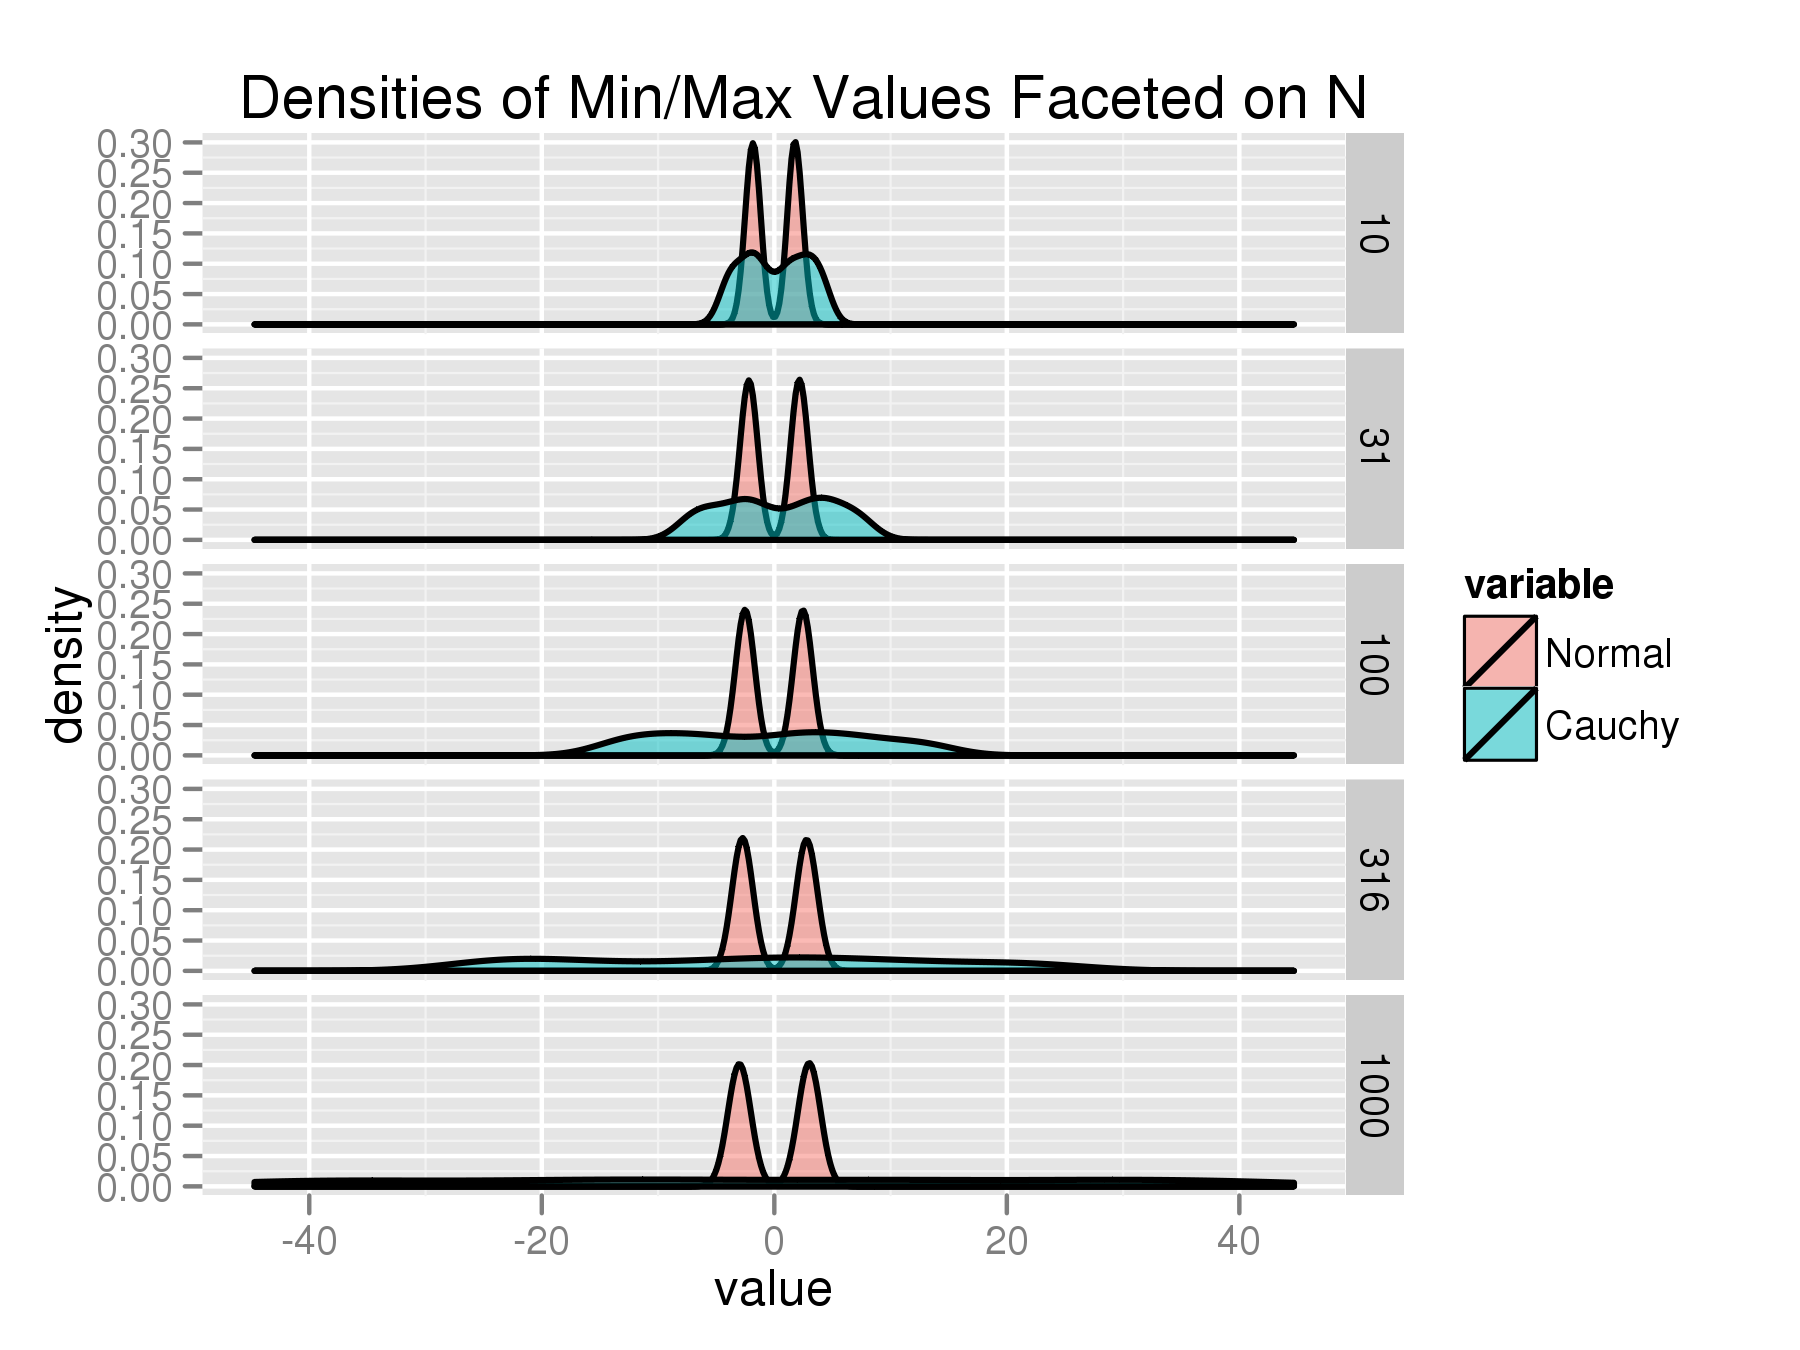
\includegraphics{./simulations/sim5.png}
\end{figure}

For $N=1000$, the Normal model typically has $u_{\Delta}$ values around 6.  In contrast, the Cauchy
model has $u_{\Delta}$ values closer to 40.  
\clearpage

Here, we plot the empirical Kolmogorov-Smirnov test statistic in the following three settings:
\begin{enumerate}
\item a standard Normal draw of size $N$ (repeated N times to get the empirical distribution)
\item the permutation $t$-statistic under Cauchy sampling (N permutations)
\item the permutation $t$-statistic under Normal sampling (N permutations)
\end{enumerate}
We also add the sum of the five unscaled, simulated bound terms ($200,000$ permutations) from the
previous section.

\begin{figure}[!ht]
  \centering
  % Created by tikzDevice version 0.6.2 on 2012-04-24 10:22:00
% !TEX encoding = UTF-8 Unicode
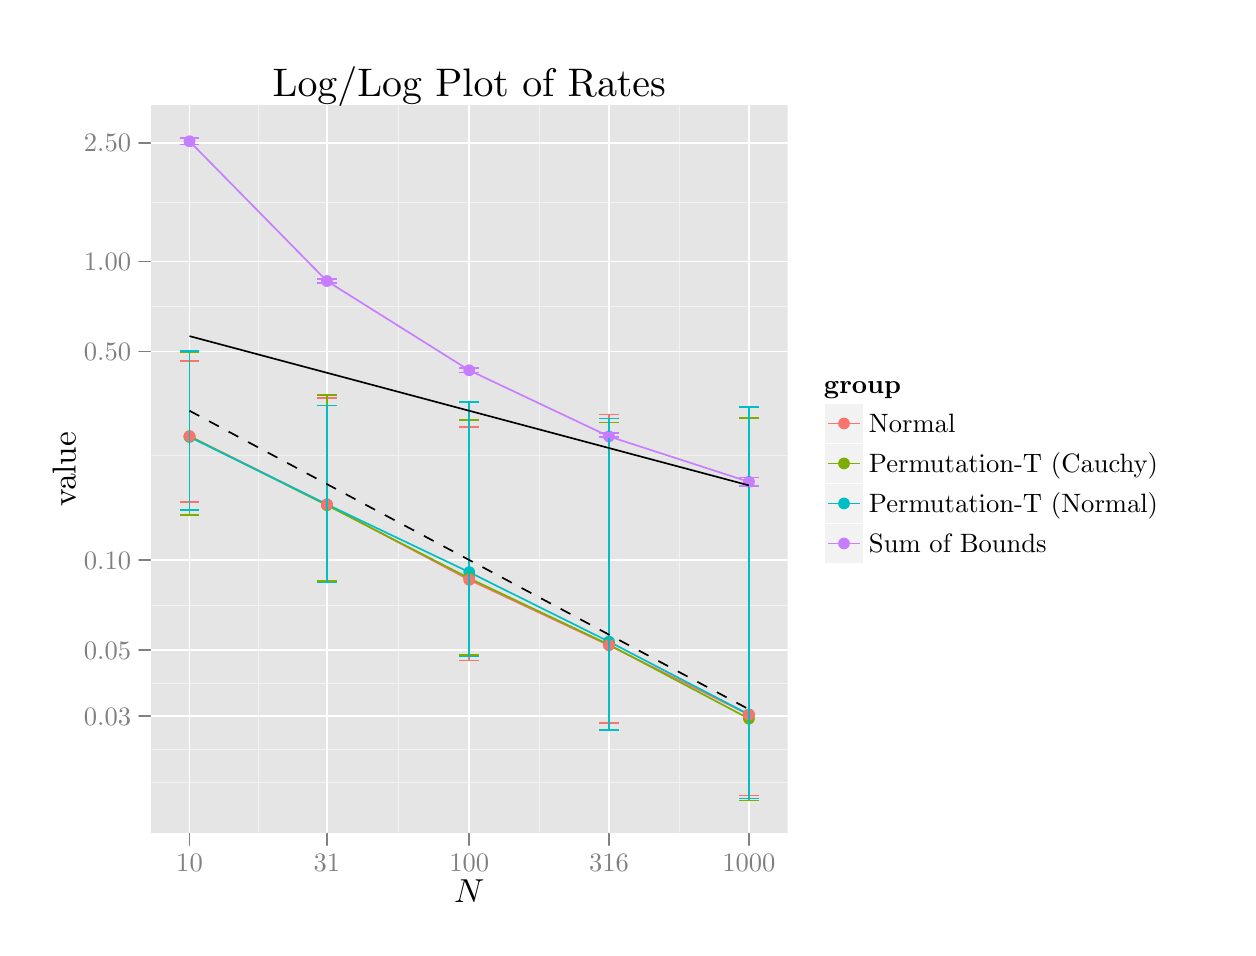
\begin{tikzpicture}[x=1pt,y=1pt]
\definecolor[named]{drawColor}{rgb}{0.00,0.00,0.00}
\definecolor[named]{fillColor}{rgb}{1.00,1.00,1.00}
\fill[color=fillColor,fill opacity=0.00,] (0,0) rectangle (433.62,325.21);
\begin{scope}
\path[clip] (  0.00,  0.00) rectangle (433.62,325.21);
\definecolor[named]{drawColor}{rgb}{0.41,0.16,0.58}
\end{scope}
\begin{scope}
\path[clip] (  0.00,  0.00) rectangle (433.62,325.21);
\definecolor[named]{drawColor}{rgb}{0.41,0.16,0.58}
\end{scope}
\begin{scope}
\path[clip] (  0.00,  0.00) rectangle (433.62,325.21);
\definecolor[named]{drawColor}{rgb}{0.41,0.16,0.58}
\end{scope}
\begin{scope}
\path[clip] (  0.00,  0.00) rectangle (433.62,325.21);
\definecolor[named]{drawColor}{rgb}{0.41,0.16,0.58}
\end{scope}
\begin{scope}
\path[clip] (  0.00,  0.00) rectangle (433.62,325.21);
\definecolor[named]{drawColor}{rgb}{0.41,0.16,0.58}
\end{scope}
\begin{scope}
\path[clip] (  0.00,  0.00) rectangle (433.62,325.21);
\definecolor[named]{drawColor}{rgb}{0.41,0.16,0.58}
\end{scope}
\begin{scope}
\path[clip] (  0.00,  0.00) rectangle (433.62,325.21);
\definecolor[named]{drawColor}{rgb}{0.41,0.16,0.58}
\end{scope}
\begin{scope}
\path[clip] (  0.00,  0.00) rectangle (433.62,325.21);
\definecolor[named]{drawColor}{rgb}{0.41,0.16,0.58}
\end{scope}
\begin{scope}
\path[clip] (  0.00,  0.00) rectangle (433.62,325.21);
\definecolor[named]{drawColor}{rgb}{0.41,0.16,0.58}
\end{scope}
\begin{scope}
\path[clip] (  0.00,  0.00) rectangle (433.62,325.21);
\definecolor[named]{drawColor}{rgb}{0.41,0.16,0.58}
\end{scope}
\begin{scope}
\path[clip] (  0.00,  0.00) rectangle (433.62,325.21);
\definecolor[named]{drawColor}{rgb}{0.41,0.16,0.58}
\end{scope}
\begin{scope}
\path[clip] (  0.00,  0.00) rectangle (433.62,325.21);
\definecolor[named]{drawColor}{rgb}{0.41,0.16,0.58}
\end{scope}
\begin{scope}
\path[clip] ( 44.49, 34.03) rectangle (274.61,297.23);
\definecolor[named]{drawColor}{rgb}{0.41,0.16,0.58}
\end{scope}
\begin{scope}
\path[clip] (  0.00,  0.00) rectangle (433.62,325.21);
\definecolor[named]{drawColor}{rgb}{0.41,0.16,0.58}
\end{scope}
\begin{scope}
\path[clip] (  0.00,  0.00) rectangle (433.62,325.21);
\definecolor[named]{drawColor}{rgb}{0.41,0.16,0.58}
\end{scope}
\begin{scope}
\path[clip] (  0.00,  0.00) rectangle (433.62,325.21);
\definecolor[named]{drawColor}{rgb}{0.41,0.16,0.58}
\end{scope}
\begin{scope}
\path[clip] (  0.00,  0.00) rectangle (433.62,325.21);
\definecolor[named]{drawColor}{rgb}{0.41,0.16,0.58}
\end{scope}
\begin{scope}
\path[clip] (  0.00,  0.00) rectangle (433.62,325.21);
\definecolor[named]{drawColor}{rgb}{0.41,0.16,0.58}
\end{scope}
\begin{scope}
\path[clip] (  0.00,  0.00) rectangle (433.62,325.21);
\definecolor[named]{drawColor}{rgb}{0.41,0.16,0.58}
\end{scope}
\begin{scope}
\path[clip] (  0.00,  0.00) rectangle (433.62,325.21);
\definecolor[named]{drawColor}{rgb}{0.41,0.16,0.58}
\end{scope}
\begin{scope}
\path[clip] (  0.00,  0.00) rectangle (433.62,325.21);
\definecolor[named]{drawColor}{rgb}{0.41,0.16,0.58}
\end{scope}
\begin{scope}
\path[clip] (  0.00,  0.00) rectangle (433.62,325.21);
\definecolor[named]{drawColor}{rgb}{0.41,0.16,0.58}
\end{scope}
\begin{scope}
\path[clip] (  0.00,  0.00) rectangle (433.62,325.21);
\definecolor[named]{drawColor}{rgb}{0.41,0.16,0.58}
\end{scope}
\begin{scope}
\path[clip] (  0.00,  0.00) rectangle (433.62,325.21);
\definecolor[named]{drawColor}{rgb}{0.41,0.16,0.58}
\end{scope}
\begin{scope}
\path[clip] (  0.00,  0.00) rectangle (433.62,325.21);
\definecolor[named]{drawColor}{rgb}{0.41,0.16,0.58}
\definecolor[named]{fillColor}{rgb}{1.00,1.00,1.00}

\draw[fill=fillColor,draw opacity=0.00,] (  0.00,  0.00) rectangle (433.62,325.21);
\end{scope}
\begin{scope}
\path[clip] (  0.00,  0.00) rectangle (433.62,325.21);
\definecolor[named]{drawColor}{rgb}{0.41,0.16,0.58}
\end{scope}
\begin{scope}
\path[clip] (  0.00,  0.00) rectangle (433.62,325.21);
\definecolor[named]{drawColor}{rgb}{0.41,0.16,0.58}
\definecolor[named]{drawColor}{rgb}{0.50,0.50,0.50}

\node[color=drawColor,anchor=base east,inner sep=0pt, outer sep=0pt, scale=  0.96] at ( 37.37, 73.13) {0.03};

\node[color=drawColor,anchor=base east,inner sep=0pt, outer sep=0pt, scale=  0.96] at ( 37.37, 97.07) {0.05};

\node[color=drawColor,anchor=base east,inner sep=0pt, outer sep=0pt, scale=  0.96] at ( 37.37,129.54) {0.10};

\node[color=drawColor,anchor=base east,inner sep=0pt, outer sep=0pt, scale=  0.96] at ( 37.37,204.94) {0.50};

\node[color=drawColor,anchor=base east,inner sep=0pt, outer sep=0pt, scale=  0.96] at ( 37.37,237.42) {1.00};

\node[color=drawColor,anchor=base east,inner sep=0pt, outer sep=0pt, scale=  0.96] at ( 37.37,280.34) {2.50};
\end{scope}
\begin{scope}
\path[clip] (  0.00,  0.00) rectangle (433.62,325.21);
\definecolor[named]{drawColor}{rgb}{0.41,0.16,0.58}
\definecolor[named]{drawColor}{rgb}{0.50,0.50,0.50}

\draw[color=drawColor,line width= 0.6pt,line cap=round,line join=round,fill opacity=0.00,] ( 40.22, 76.44) -- ( 44.49, 76.44);

\draw[color=drawColor,line width= 0.6pt,line cap=round,line join=round,fill opacity=0.00,] ( 40.22,100.37) -- ( 44.49,100.37);

\draw[color=drawColor,line width= 0.6pt,line cap=round,line join=round,fill opacity=0.00,] ( 40.22,132.85) -- ( 44.49,132.85);

\draw[color=drawColor,line width= 0.6pt,line cap=round,line join=round,fill opacity=0.00,] ( 40.22,208.25) -- ( 44.49,208.25);

\draw[color=drawColor,line width= 0.6pt,line cap=round,line join=round,fill opacity=0.00,] ( 40.22,240.72) -- ( 44.49,240.72);

\draw[color=drawColor,line width= 0.6pt,line cap=round,line join=round,fill opacity=0.00,] ( 40.22,283.65) -- ( 44.49,283.65);
\end{scope}
\begin{scope}
\path[clip] (  0.00,  0.00) rectangle (433.62,325.21);
\definecolor[named]{drawColor}{rgb}{0.41,0.16,0.58}
\end{scope}
\begin{scope}
\path[clip] (  0.00,  0.00) rectangle (433.62,325.21);
\definecolor[named]{drawColor}{rgb}{0.41,0.16,0.58}
\end{scope}
\begin{scope}
\path[clip] (  0.00,  0.00) rectangle (433.62,325.21);
\definecolor[named]{drawColor}{rgb}{0.41,0.16,0.58}
\end{scope}
\begin{scope}
\path[clip] (  0.00,  0.00) rectangle (433.62,325.21);
\definecolor[named]{drawColor}{rgb}{0.41,0.16,0.58}
\end{scope}
\begin{scope}
\path[clip] (  0.00,  0.00) rectangle (433.62,325.21);
\definecolor[named]{drawColor}{rgb}{0.41,0.16,0.58}
\end{scope}
\begin{scope}
\path[clip] ( 44.49, 34.03) rectangle (274.61,297.23);
\definecolor[named]{drawColor}{rgb}{0.41,0.16,0.58}
\definecolor[named]{fillColor}{rgb}{0.90,0.90,0.90}

\draw[fill=fillColor,draw opacity=0.00,] ( 44.49, 34.03) rectangle (274.61,297.23);
\definecolor[named]{drawColor}{rgb}{0.95,0.95,0.95}

\draw[color=drawColor,line width= 0.3pt,line cap=round,line join=round,fill opacity=0.00,] ( 44.49, 52.51) --
	(274.61, 52.51);

\draw[color=drawColor,line width= 0.3pt,line cap=round,line join=round,fill opacity=0.00,] ( 44.49, 64.47) --
	(274.61, 64.47);

\draw[color=drawColor,line width= 0.3pt,line cap=round,line join=round,fill opacity=0.00,] ( 44.49, 88.41) --
	(274.61, 88.41);

\draw[color=drawColor,line width= 0.3pt,line cap=round,line join=round,fill opacity=0.00,] ( 44.49,116.61) --
	(274.61,116.61);

\draw[color=drawColor,line width= 0.3pt,line cap=round,line join=round,fill opacity=0.00,] ( 44.49,170.55) --
	(274.61,170.55);

\draw[color=drawColor,line width= 0.3pt,line cap=round,line join=round,fill opacity=0.00,] ( 44.49,224.49) --
	(274.61,224.49);

\draw[color=drawColor,line width= 0.3pt,line cap=round,line join=round,fill opacity=0.00,] ( 44.49,262.19) --
	(274.61,262.19);

\draw[color=drawColor,line width= 0.3pt,line cap=round,line join=round,fill opacity=0.00,] ( 83.31, 34.03) --
	( 83.31,297.23);

\draw[color=drawColor,line width= 0.3pt,line cap=round,line join=round,fill opacity=0.00,] (133.85, 34.03) --
	(133.85,297.23);

\draw[color=drawColor,line width= 0.3pt,line cap=round,line join=round,fill opacity=0.00,] (184.80, 34.03) --
	(184.80,297.23);

\draw[color=drawColor,line width= 0.3pt,line cap=round,line join=round,fill opacity=0.00,] (235.33, 34.03) --
	(235.33,297.23);
\definecolor[named]{drawColor}{rgb}{1.00,1.00,1.00}

\draw[color=drawColor,line width= 0.6pt,line cap=round,line join=round,fill opacity=0.00,] ( 44.49, 76.44) --
	(274.61, 76.44);

\draw[color=drawColor,line width= 0.6pt,line cap=round,line join=round,fill opacity=0.00,] ( 44.49,100.37) --
	(274.61,100.37);

\draw[color=drawColor,line width= 0.6pt,line cap=round,line join=round,fill opacity=0.00,] ( 44.49,132.85) --
	(274.61,132.85);

\draw[color=drawColor,line width= 0.6pt,line cap=round,line join=round,fill opacity=0.00,] ( 44.49,208.25) --
	(274.61,208.25);

\draw[color=drawColor,line width= 0.6pt,line cap=round,line join=round,fill opacity=0.00,] ( 44.49,240.72) --
	(274.61,240.72);

\draw[color=drawColor,line width= 0.6pt,line cap=round,line join=round,fill opacity=0.00,] ( 44.49,283.65) --
	(274.61,283.65);

\draw[color=drawColor,line width= 0.6pt,line cap=round,line join=round,fill opacity=0.00,] ( 58.48, 34.03) --
	( 58.48,297.23);

\draw[color=drawColor,line width= 0.6pt,line cap=round,line join=round,fill opacity=0.00,] (108.14, 34.03) --
	(108.14,297.23);

\draw[color=drawColor,line width= 0.6pt,line cap=round,line join=round,fill opacity=0.00,] (159.55, 34.03) --
	(159.55,297.23);

\draw[color=drawColor,line width= 0.6pt,line cap=round,line join=round,fill opacity=0.00,] (210.05, 34.03) --
	(210.05,297.23);

\draw[color=drawColor,line width= 0.6pt,line cap=round,line join=round,fill opacity=0.00,] (260.62, 34.03) --
	(260.62,297.23);
\definecolor[named]{drawColor}{rgb}{0.97,0.46,0.43}

\draw[color=drawColor,line width= 0.6pt,line join=round,fill opacity=0.00,] ( 58.48,177.61) --
	(108.14,152.89) --
	(159.55,125.69) --
	(210.05,102.01) --
	(260.62, 76.96);
\definecolor[named]{drawColor}{rgb}{0.49,0.68,0.00}

\draw[color=drawColor,line width= 0.6pt,line join=round,fill opacity=0.00,] ( 58.48,177.55) --
	(108.14,152.64) --
	(159.55,126.25) --
	(210.05,102.26) --
	(260.62, 75.52);
\definecolor[named]{drawColor}{rgb}{0.00,0.75,0.77}

\draw[color=drawColor,line width= 0.6pt,line join=round,fill opacity=0.00,] ( 58.48,177.31) --
	(108.14,152.96) --
	(159.55,128.45) --
	(210.05,103.35) --
	(260.62, 77.05);
\definecolor[named]{drawColor}{rgb}{0.78,0.49,1.00}

\draw[color=drawColor,line width= 0.6pt,line join=round,fill opacity=0.00,] ( 58.48,284.15) --
	(108.14,233.65) --
	(159.55,201.40) --
	(210.05,177.51) --
	(260.62,161.10);
\definecolor[named]{fillColor}{rgb}{0.00,0.75,0.77}

\draw[fill=fillColor,draw opacity=0.00,] ( 58.48,177.31) circle (  2.13);
\definecolor[named]{fillColor}{rgb}{0.49,0.68,0.00}

\draw[fill=fillColor,draw opacity=0.00,] ( 58.48,177.55) circle (  2.13);
\definecolor[named]{fillColor}{rgb}{0.97,0.46,0.43}

\draw[fill=fillColor,draw opacity=0.00,] ( 58.48,177.61) circle (  2.13);
\definecolor[named]{fillColor}{rgb}{0.00,0.75,0.77}

\draw[fill=fillColor,draw opacity=0.00,] (108.14,152.96) circle (  2.13);
\definecolor[named]{fillColor}{rgb}{0.49,0.68,0.00}

\draw[fill=fillColor,draw opacity=0.00,] (108.14,152.64) circle (  2.13);
\definecolor[named]{fillColor}{rgb}{0.97,0.46,0.43}

\draw[fill=fillColor,draw opacity=0.00,] (108.14,152.89) circle (  2.13);
\definecolor[named]{fillColor}{rgb}{0.00,0.75,0.77}

\draw[fill=fillColor,draw opacity=0.00,] (159.55,128.45) circle (  2.13);
\definecolor[named]{fillColor}{rgb}{0.49,0.68,0.00}

\draw[fill=fillColor,draw opacity=0.00,] (159.55,126.25) circle (  2.13);
\definecolor[named]{fillColor}{rgb}{0.97,0.46,0.43}

\draw[fill=fillColor,draw opacity=0.00,] (159.55,125.69) circle (  2.13);
\definecolor[named]{fillColor}{rgb}{0.00,0.75,0.77}

\draw[fill=fillColor,draw opacity=0.00,] (210.05,103.35) circle (  2.13);
\definecolor[named]{fillColor}{rgb}{0.49,0.68,0.00}

\draw[fill=fillColor,draw opacity=0.00,] (210.05,102.26) circle (  2.13);
\definecolor[named]{fillColor}{rgb}{0.97,0.46,0.43}

\draw[fill=fillColor,draw opacity=0.00,] (210.05,102.01) circle (  2.13);
\definecolor[named]{fillColor}{rgb}{0.00,0.75,0.77}

\draw[fill=fillColor,draw opacity=0.00,] (260.62, 77.05) circle (  2.13);
\definecolor[named]{fillColor}{rgb}{0.49,0.68,0.00}

\draw[fill=fillColor,draw opacity=0.00,] (260.62, 75.52) circle (  2.13);
\definecolor[named]{fillColor}{rgb}{0.97,0.46,0.43}

\draw[fill=fillColor,draw opacity=0.00,] (260.62, 76.96) circle (  2.13);
\definecolor[named]{fillColor}{rgb}{0.78,0.49,1.00}

\draw[fill=fillColor,draw opacity=0.00,] ( 58.48,284.15) circle (  2.13);

\draw[fill=fillColor,draw opacity=0.00,] (108.14,233.65) circle (  2.13);

\draw[fill=fillColor,draw opacity=0.00,] (159.55,201.40) circle (  2.13);

\draw[fill=fillColor,draw opacity=0.00,] (210.05,177.51) circle (  2.13);

\draw[fill=fillColor,draw opacity=0.00,] (260.62,161.10) circle (  2.13);
\definecolor[named]{drawColor}{rgb}{0.97,0.46,0.43}

\draw[color=drawColor,line width= 0.6pt,line join=round,fill opacity=0.00,] ( 54.95,204.74) --
	( 62.02,204.74);

\draw[color=drawColor,line width= 0.6pt,line join=round,fill opacity=0.00,] ( 58.48,204.74) --
	( 58.48,153.80);

\draw[color=drawColor,line width= 0.6pt,line join=round,fill opacity=0.00,] ( 54.95,153.80) --
	( 62.02,153.80);

\draw[color=drawColor,line width= 0.6pt,line join=round,fill opacity=0.00,] (104.61,191.45) --
	(111.68,191.45);

\draw[color=drawColor,line width= 0.6pt,line join=round,fill opacity=0.00,] (108.14,191.45) --
	(108.14,125.00);

\draw[color=drawColor,line width= 0.6pt,line join=round,fill opacity=0.00,] (104.61,125.00) --
	(111.68,125.00);

\draw[color=drawColor,line width= 0.6pt,line join=round,fill opacity=0.00,] (156.01,181.01) --
	(163.09,181.01);

\draw[color=drawColor,line width= 0.6pt,line join=round,fill opacity=0.00,] (159.55,181.01) --
	(159.55, 96.56);

\draw[color=drawColor,line width= 0.6pt,line join=round,fill opacity=0.00,] (156.01, 96.56) --
	(163.09, 96.56);

\draw[color=drawColor,line width= 0.6pt,line join=round,fill opacity=0.00,] (206.51,185.42) --
	(213.59,185.42);

\draw[color=drawColor,line width= 0.6pt,line join=round,fill opacity=0.00,] (210.05,185.42) --
	(210.05, 73.96);

\draw[color=drawColor,line width= 0.6pt,line join=round,fill opacity=0.00,] (206.51, 73.96) --
	(213.59, 73.96);

\draw[color=drawColor,line width= 0.6pt,line join=round,fill opacity=0.00,] (257.08,184.36) --
	(264.15,184.36);

\draw[color=drawColor,line width= 0.6pt,line join=round,fill opacity=0.00,] (260.62,184.36) --
	(260.62, 47.72);

\draw[color=drawColor,line width= 0.6pt,line join=round,fill opacity=0.00,] (257.08, 47.72) --
	(264.15, 47.72);
\definecolor[named]{drawColor}{rgb}{0.49,0.68,0.00}

\draw[color=drawColor,line width= 0.6pt,line join=round,fill opacity=0.00,] ( 54.95,207.80) --
	( 62.02,207.80);

\draw[color=drawColor,line width= 0.6pt,line join=round,fill opacity=0.00,] ( 58.48,207.80) --
	( 58.48,149.16);

\draw[color=drawColor,line width= 0.6pt,line join=round,fill opacity=0.00,] ( 54.95,149.16) --
	( 62.02,149.16);

\draw[color=drawColor,line width= 0.6pt,line join=round,fill opacity=0.00,] (104.61,192.36) --
	(111.68,192.36);

\draw[color=drawColor,line width= 0.6pt,line join=round,fill opacity=0.00,] (108.14,192.36) --
	(108.14,125.24);

\draw[color=drawColor,line width= 0.6pt,line join=round,fill opacity=0.00,] (104.61,125.24) --
	(111.68,125.24);

\draw[color=drawColor,line width= 0.6pt,line join=round,fill opacity=0.00,] (156.01,183.42) --
	(163.09,183.42);

\draw[color=drawColor,line width= 0.6pt,line join=round,fill opacity=0.00,] (159.55,183.42) --
	(159.55, 98.53);

\draw[color=drawColor,line width= 0.6pt,line join=round,fill opacity=0.00,] (156.01, 98.53) --
	(163.09, 98.53);

\draw[color=drawColor,line width= 0.6pt,line join=round,fill opacity=0.00,] (206.51,182.54) --
	(213.59,182.54);

\draw[color=drawColor,line width= 0.6pt,line join=round,fill opacity=0.00,] (210.05,182.54) --
	(210.05, 71.65);

\draw[color=drawColor,line width= 0.6pt,line join=round,fill opacity=0.00,] (206.51, 71.65) --
	(213.59, 71.65);

\draw[color=drawColor,line width= 0.6pt,line join=round,fill opacity=0.00,] (257.08,184.20) --
	(264.15,184.20);

\draw[color=drawColor,line width= 0.6pt,line join=round,fill opacity=0.00,] (260.62,184.20) --
	(260.62, 46.00);

\draw[color=drawColor,line width= 0.6pt,line join=round,fill opacity=0.00,] (257.08, 46.00) --
	(264.15, 46.00);
\definecolor[named]{drawColor}{rgb}{0.00,0.75,0.77}

\draw[color=drawColor,line width= 0.6pt,line join=round,fill opacity=0.00,] ( 54.95,208.27) --
	( 62.02,208.27);

\draw[color=drawColor,line width= 0.6pt,line join=round,fill opacity=0.00,] ( 58.48,208.27) --
	( 58.48,150.80);

\draw[color=drawColor,line width= 0.6pt,line join=round,fill opacity=0.00,] ( 54.95,150.80) --
	( 62.02,150.80);

\draw[color=drawColor,line width= 0.6pt,line join=round,fill opacity=0.00,] (104.61,188.64) --
	(111.68,188.64);

\draw[color=drawColor,line width= 0.6pt,line join=round,fill opacity=0.00,] (108.14,188.64) --
	(108.14,124.72);

\draw[color=drawColor,line width= 0.6pt,line join=round,fill opacity=0.00,] (104.61,124.72) --
	(111.68,124.72);

\draw[color=drawColor,line width= 0.6pt,line join=round,fill opacity=0.00,] (156.01,189.99) --
	(163.09,189.99);

\draw[color=drawColor,line width= 0.6pt,line join=round,fill opacity=0.00,] (159.55,189.99) --
	(159.55, 98.00);

\draw[color=drawColor,line width= 0.6pt,line join=round,fill opacity=0.00,] (156.01, 98.00) --
	(163.09, 98.00);

\draw[color=drawColor,line width= 0.6pt,line join=round,fill opacity=0.00,] (206.51,183.95) --
	(213.59,183.95);

\draw[color=drawColor,line width= 0.6pt,line join=round,fill opacity=0.00,] (210.05,183.95) --
	(210.05, 71.48);

\draw[color=drawColor,line width= 0.6pt,line join=round,fill opacity=0.00,] (206.51, 71.48) --
	(213.59, 71.48);

\draw[color=drawColor,line width= 0.6pt,line join=round,fill opacity=0.00,] (257.08,188.23) --
	(264.15,188.23);

\draw[color=drawColor,line width= 0.6pt,line join=round,fill opacity=0.00,] (260.62,188.23) --
	(260.62, 46.65);

\draw[color=drawColor,line width= 0.6pt,line join=round,fill opacity=0.00,] (257.08, 46.65) --
	(264.15, 46.65);
\definecolor[named]{drawColor}{rgb}{0.78,0.49,1.00}

\draw[color=drawColor,line width= 0.6pt,line join=round,fill opacity=0.00,] ( 54.95,285.27) --
	( 62.02,285.27);

\draw[color=drawColor,line width= 0.6pt,line join=round,fill opacity=0.00,] ( 58.48,285.27) --
	( 58.48,283.02);

\draw[color=drawColor,line width= 0.6pt,line join=round,fill opacity=0.00,] ( 54.95,283.02) --
	( 62.02,283.02);

\draw[color=drawColor,line width= 0.6pt,line join=round,fill opacity=0.00,] (104.61,234.28) --
	(111.68,234.28);

\draw[color=drawColor,line width= 0.6pt,line join=round,fill opacity=0.00,] (108.14,234.28) --
	(108.14,233.01);

\draw[color=drawColor,line width= 0.6pt,line join=round,fill opacity=0.00,] (104.61,233.01) --
	(111.68,233.01);

\draw[color=drawColor,line width= 0.6pt,line join=round,fill opacity=0.00,] (156.01,202.24) --
	(163.09,202.24);

\draw[color=drawColor,line width= 0.6pt,line join=round,fill opacity=0.00,] (159.55,202.24) --
	(159.55,200.59);

\draw[color=drawColor,line width= 0.6pt,line join=round,fill opacity=0.00,] (156.01,200.59) --
	(163.09,200.59);

\draw[color=drawColor,line width= 0.6pt,line join=round,fill opacity=0.00,] (206.51,178.78) --
	(213.59,178.78);

\draw[color=drawColor,line width= 0.6pt,line join=round,fill opacity=0.00,] (210.05,178.78) --
	(210.05,177.26);

\draw[color=drawColor,line width= 0.6pt,line join=round,fill opacity=0.00,] (206.51,177.26) --
	(213.59,177.26);

\draw[color=drawColor,line width= 0.6pt,line join=round,fill opacity=0.00,] (257.08,162.61) --
	(264.15,162.61);

\draw[color=drawColor,line width= 0.6pt,line join=round,fill opacity=0.00,] (260.62,162.61) --
	(260.62,159.55);

\draw[color=drawColor,line width= 0.6pt,line join=round,fill opacity=0.00,] (257.08,159.55) --
	(264.15,159.55);
\definecolor[named]{drawColor}{rgb}{0.00,0.00,0.00}

\draw[color=drawColor,line width= 0.6pt,dash pattern=on 4pt off 4pt ,line join=round,fill opacity=0.00,] ( 58.48,186.78) --
	( 58.48,186.78) --
	( 58.48,186.78) --
	( 58.48,186.78) --
	(108.14,160.28) --
	(108.14,160.28) --
	(108.14,160.28) --
	(108.14,160.28) --
	(159.55,132.85) --
	(159.55,132.85) --
	(159.55,132.85) --
	(159.55,132.85) --
	(210.05,105.89) --
	(210.05,105.89) --
	(210.05,105.89) --
	(210.05,105.89) --
	(260.62, 78.91) --
	(260.62, 78.91) --
	(260.62, 78.91) --
	(260.62, 78.91);

\draw[color=drawColor,line width= 0.6pt,line join=round,fill opacity=0.00,] ( 58.48,213.75) --
	( 58.48,213.75) --
	( 58.48,213.75) --
	( 58.48,213.75) --
	(108.14,200.50) --
	(108.14,200.50) --
	(108.14,200.50) --
	(108.14,200.50) --
	(159.55,186.78) --
	(159.55,186.78) --
	(159.55,186.78) --
	(159.55,186.78) --
	(210.05,173.31) --
	(210.05,173.31) --
	(210.05,173.31) --
	(210.05,173.31) --
	(260.62,159.82) --
	(260.62,159.82) --
	(260.62,159.82) --
	(260.62,159.82);
\end{scope}
\begin{scope}
\path[clip] (  0.00,  0.00) rectangle (433.62,325.21);
\definecolor[named]{drawColor}{rgb}{0.41,0.16,0.58}
\end{scope}
\begin{scope}
\path[clip] (  0.00,  0.00) rectangle (433.62,325.21);
\definecolor[named]{drawColor}{rgb}{0.41,0.16,0.58}
\definecolor[named]{drawColor}{rgb}{0.50,0.50,0.50}

\node[color=drawColor,anchor=base,inner sep=0pt, outer sep=0pt, scale=  0.96] at ( 58.48, 20.31) {10};

\node[color=drawColor,anchor=base,inner sep=0pt, outer sep=0pt, scale=  0.96] at (108.14, 20.31) {31};

\node[color=drawColor,anchor=base,inner sep=0pt, outer sep=0pt, scale=  0.96] at (159.55, 20.31) {100};

\node[color=drawColor,anchor=base,inner sep=0pt, outer sep=0pt, scale=  0.96] at (210.05, 20.31) {316};

\node[color=drawColor,anchor=base,inner sep=0pt, outer sep=0pt, scale=  0.96] at (260.62, 20.31) {1000};
\end{scope}
\begin{scope}
\path[clip] (  0.00,  0.00) rectangle (433.62,325.21);
\definecolor[named]{drawColor}{rgb}{0.41,0.16,0.58}
\definecolor[named]{drawColor}{rgb}{0.50,0.50,0.50}

\draw[color=drawColor,line width= 0.6pt,line cap=round,line join=round,fill opacity=0.00,] ( 58.48, 29.77) -- ( 58.48, 34.03);

\draw[color=drawColor,line width= 0.6pt,line cap=round,line join=round,fill opacity=0.00,] (108.14, 29.77) -- (108.14, 34.03);

\draw[color=drawColor,line width= 0.6pt,line cap=round,line join=round,fill opacity=0.00,] (159.55, 29.77) -- (159.55, 34.03);

\draw[color=drawColor,line width= 0.6pt,line cap=round,line join=round,fill opacity=0.00,] (210.05, 29.77) -- (210.05, 34.03);

\draw[color=drawColor,line width= 0.6pt,line cap=round,line join=round,fill opacity=0.00,] (260.62, 29.77) -- (260.62, 34.03);
\end{scope}
\begin{scope}
\path[clip] (  0.00,  0.00) rectangle (433.62,325.21);
\definecolor[named]{drawColor}{rgb}{0.41,0.16,0.58}
\end{scope}
\begin{scope}
\path[clip] (  0.00,  0.00) rectangle (433.62,325.21);
\definecolor[named]{drawColor}{rgb}{0.41,0.16,0.58}
\end{scope}
\begin{scope}
\path[clip] (  0.00,  0.00) rectangle (433.62,325.21);
\definecolor[named]{drawColor}{rgb}{0.41,0.16,0.58}
\end{scope}
\begin{scope}
\path[clip] (  0.00,  0.00) rectangle (433.62,325.21);
\definecolor[named]{drawColor}{rgb}{0.41,0.16,0.58}
\definecolor[named]{drawColor}{rgb}{0.00,0.00,0.00}

\node[color=drawColor,anchor=base,inner sep=0pt, outer sep=0pt, scale=  1.44] at (159.55,300.24) {Log/Log Plot of Rates};
\end{scope}
\begin{scope}
\path[clip] (  0.00,  0.00) rectangle (433.62,325.21);
\definecolor[named]{drawColor}{rgb}{0.41,0.16,0.58}
\end{scope}
\begin{scope}
\path[clip] (  0.00,  0.00) rectangle (433.62,325.21);
\definecolor[named]{drawColor}{rgb}{0.41,0.16,0.58}
\definecolor[named]{drawColor}{rgb}{0.00,0.00,0.00}

\node[color=drawColor,anchor=base,inner sep=0pt, outer sep=0pt, scale=  1.20] at (159.55,  9.03) {$N$};
\end{scope}
\begin{scope}
\path[clip] (  0.00,  0.00) rectangle (433.62,325.21);
\definecolor[named]{drawColor}{rgb}{0.41,0.16,0.58}
\end{scope}
\begin{scope}
\path[clip] (  0.00,  0.00) rectangle (433.62,325.21);
\definecolor[named]{drawColor}{rgb}{0.41,0.16,0.58}
\definecolor[named]{drawColor}{rgb}{0.00,0.00,0.00}

\node[rotate= 90.00,color=drawColor,anchor=base,inner sep=0pt, outer sep=0pt, scale=  1.20] at ( 17.30,165.63) {value};
\end{scope}
\begin{scope}
\path[clip] (  0.00,  0.00) rectangle (433.62,325.21);
\definecolor[named]{drawColor}{rgb}{0.41,0.16,0.58}
\end{scope}
\begin{scope}
\path[clip] (  0.00,  0.00) rectangle (433.62,325.21);
\definecolor[named]{drawColor}{rgb}{0.41,0.16,0.58}
\end{scope}
\begin{scope}
\path[clip] (  0.00,  0.00) rectangle (433.62,325.21);
\definecolor[named]{drawColor}{rgb}{0.41,0.16,0.58}
\end{scope}
\begin{scope}
\path[clip] (  0.00,  0.00) rectangle (433.62,325.21);
\definecolor[named]{drawColor}{rgb}{0.41,0.16,0.58}
\end{scope}
\begin{scope}
\path[clip] (  0.00,  0.00) rectangle (433.62,325.21);
\definecolor[named]{drawColor}{rgb}{0.41,0.16,0.58}
\end{scope}
\begin{scope}
\path[clip] (  0.00,  0.00) rectangle (433.62,325.21);
\definecolor[named]{drawColor}{rgb}{0.41,0.16,0.58}
\end{scope}
\begin{scope}
\path[clip] (  0.00,  0.00) rectangle (433.62,325.21);
\definecolor[named]{drawColor}{rgb}{0.41,0.16,0.58}
\end{scope}
\begin{scope}
\path[clip] (  0.00,  0.00) rectangle (433.62,325.21);
\definecolor[named]{drawColor}{rgb}{0.41,0.16,0.58}
\end{scope}
\begin{scope}
\path[clip] (  0.00,  0.00) rectangle (433.62,325.21);
\definecolor[named]{drawColor}{rgb}{0.41,0.16,0.58}
\end{scope}
\begin{scope}
\path[clip] (  0.00,  0.00) rectangle (433.62,325.21);
\definecolor[named]{drawColor}{rgb}{0.41,0.16,0.58}
\end{scope}
\begin{scope}
\path[clip] (  0.00,  0.00) rectangle (433.62,325.21);
\definecolor[named]{drawColor}{rgb}{0.41,0.16,0.58}
\end{scope}
\begin{scope}
\path[clip] (  0.00,  0.00) rectangle (433.62,325.21);
\definecolor[named]{drawColor}{rgb}{0.41,0.16,0.58}
\end{scope}
\begin{scope}
\path[clip] (  0.00,  0.00) rectangle (433.62,325.21);
\definecolor[named]{drawColor}{rgb}{0.41,0.16,0.58}
\end{scope}
\begin{scope}
\path[clip] (  0.00,  0.00) rectangle (433.62,325.21);
\definecolor[named]{drawColor}{rgb}{0.41,0.16,0.58}
\end{scope}
\begin{scope}
\path[clip] (  0.00,  0.00) rectangle (433.62,325.21);
\definecolor[named]{drawColor}{rgb}{0.41,0.16,0.58}
\end{scope}
\begin{scope}
\path[clip] (  0.00,  0.00) rectangle (433.62,325.21);
\definecolor[named]{drawColor}{rgb}{0.41,0.16,0.58}
\end{scope}
\begin{scope}
\path[clip] (  0.00,  0.00) rectangle (433.62,325.21);
\definecolor[named]{drawColor}{rgb}{0.41,0.16,0.58}
\end{scope}
\begin{scope}
\path[clip] (  0.00,  0.00) rectangle (433.62,325.21);
\definecolor[named]{drawColor}{rgb}{0.41,0.16,0.58}
\end{scope}
\begin{scope}
\path[clip] (  0.00,  0.00) rectangle (433.62,325.21);
\definecolor[named]{drawColor}{rgb}{0.41,0.16,0.58}
\end{scope}
\begin{scope}
\path[clip] (  0.00,  0.00) rectangle (433.62,325.21);
\definecolor[named]{drawColor}{rgb}{0.41,0.16,0.58}
\end{scope}
\begin{scope}
\path[clip] (  0.00,  0.00) rectangle (433.62,325.21);
\definecolor[named]{drawColor}{rgb}{0.41,0.16,0.58}
\end{scope}
\begin{scope}
\path[clip] (  0.00,  0.00) rectangle (433.62,325.21);
\definecolor[named]{drawColor}{rgb}{0.41,0.16,0.58}
\end{scope}
\begin{scope}
\path[clip] (  0.00,  0.00) rectangle (433.62,325.21);
\definecolor[named]{drawColor}{rgb}{0.41,0.16,0.58}
\end{scope}
\begin{scope}
\path[clip] (  0.00,  0.00) rectangle (433.62,325.21);
\definecolor[named]{drawColor}{rgb}{0.41,0.16,0.58}
\end{scope}
\begin{scope}
\path[clip] (  0.00,  0.00) rectangle (433.62,325.21);
\definecolor[named]{drawColor}{rgb}{0.41,0.16,0.58}
\definecolor[named]{drawColor}{rgb}{1.00,1.00,1.00}

\draw[color=drawColor,line width= 0.6pt,line cap=round,line join=round,fill opacity=0.00,] (283.48,127.34) rectangle (412.71,203.93);
\end{scope}
\begin{scope}
\path[clip] (  0.00,  0.00) rectangle (433.62,325.21);
\definecolor[named]{drawColor}{rgb}{0.41,0.16,0.58}
\definecolor[named]{drawColor}{rgb}{0.00,0.00,0.00}

\node[color=drawColor,anchor=base west,inner sep=0pt, outer sep=0pt, scale=  0.96] at (287.75,193.03) {\bfseries group};
\end{scope}
\begin{scope}
\path[clip] (  0.00,  0.00) rectangle (433.62,325.21);
\definecolor[named]{drawColor}{rgb}{0.41,0.16,0.58}
\definecolor[named]{drawColor}{rgb}{1.00,1.00,1.00}
\definecolor[named]{fillColor}{rgb}{0.95,0.95,0.95}

\draw[color=drawColor,line width= 0.6pt,line cap=round,line join=round,fill=fillColor,] (287.75,174.97) rectangle (302.20,189.42);
\end{scope}
\begin{scope}
\path[clip] (  0.00,  0.00) rectangle (433.62,325.21);
\definecolor[named]{drawColor}{rgb}{0.41,0.16,0.58}
\definecolor[named]{drawColor}{rgb}{0.97,0.46,0.43}

\draw[color=drawColor,line width= 0.6pt,line join=round,fill opacity=0.00,] (289.20,182.19) -- (300.76,182.19);
\end{scope}
\begin{scope}
\path[clip] (  0.00,  0.00) rectangle (433.62,325.21);
\definecolor[named]{drawColor}{rgb}{0.41,0.16,0.58}
\definecolor[named]{fillColor}{rgb}{0.97,0.46,0.43}

\draw[fill=fillColor,draw opacity=0.00,] (294.98,182.19) circle (  2.13);
\end{scope}
\begin{scope}
\path[clip] (  0.00,  0.00) rectangle (433.62,325.21);
\definecolor[named]{drawColor}{rgb}{0.41,0.16,0.58}
\definecolor[named]{drawColor}{rgb}{0.97,0.46,0.43}

\draw[color=drawColor,line width= 0.6pt,line join=round,fill opacity=0.00,] (289.20,182.19) -- (300.76,182.19);
\end{scope}
\begin{scope}
\path[clip] (  0.00,  0.00) rectangle (433.62,325.21);
\definecolor[named]{drawColor}{rgb}{0.41,0.16,0.58}
\definecolor[named]{drawColor}{rgb}{1.00,1.00,1.00}
\definecolor[named]{fillColor}{rgb}{0.95,0.95,0.95}

\draw[color=drawColor,line width= 0.6pt,line cap=round,line join=round,fill=fillColor,] (287.75,160.51) rectangle (302.20,174.97);
\end{scope}
\begin{scope}
\path[clip] (  0.00,  0.00) rectangle (433.62,325.21);
\definecolor[named]{drawColor}{rgb}{0.41,0.16,0.58}
\definecolor[named]{drawColor}{rgb}{0.49,0.68,0.00}

\draw[color=drawColor,line width= 0.6pt,line join=round,fill opacity=0.00,] (289.20,167.74) -- (300.76,167.74);
\end{scope}
\begin{scope}
\path[clip] (  0.00,  0.00) rectangle (433.62,325.21);
\definecolor[named]{drawColor}{rgb}{0.41,0.16,0.58}
\definecolor[named]{fillColor}{rgb}{0.49,0.68,0.00}

\draw[fill=fillColor,draw opacity=0.00,] (294.98,167.74) circle (  2.13);
\end{scope}
\begin{scope}
\path[clip] (  0.00,  0.00) rectangle (433.62,325.21);
\definecolor[named]{drawColor}{rgb}{0.41,0.16,0.58}
\definecolor[named]{drawColor}{rgb}{0.49,0.68,0.00}

\draw[color=drawColor,line width= 0.6pt,line join=round,fill opacity=0.00,] (289.20,167.74) -- (300.76,167.74);
\end{scope}
\begin{scope}
\path[clip] (  0.00,  0.00) rectangle (433.62,325.21);
\definecolor[named]{drawColor}{rgb}{0.41,0.16,0.58}
\definecolor[named]{drawColor}{rgb}{1.00,1.00,1.00}
\definecolor[named]{fillColor}{rgb}{0.95,0.95,0.95}

\draw[color=drawColor,line width= 0.6pt,line cap=round,line join=round,fill=fillColor,] (287.75,146.06) rectangle (302.20,160.51);
\end{scope}
\begin{scope}
\path[clip] (  0.00,  0.00) rectangle (433.62,325.21);
\definecolor[named]{drawColor}{rgb}{0.41,0.16,0.58}
\definecolor[named]{drawColor}{rgb}{0.00,0.75,0.77}

\draw[color=drawColor,line width= 0.6pt,line join=round,fill opacity=0.00,] (289.20,153.29) -- (300.76,153.29);
\end{scope}
\begin{scope}
\path[clip] (  0.00,  0.00) rectangle (433.62,325.21);
\definecolor[named]{drawColor}{rgb}{0.41,0.16,0.58}
\definecolor[named]{fillColor}{rgb}{0.00,0.75,0.77}

\draw[fill=fillColor,draw opacity=0.00,] (294.98,153.29) circle (  2.13);
\end{scope}
\begin{scope}
\path[clip] (  0.00,  0.00) rectangle (433.62,325.21);
\definecolor[named]{drawColor}{rgb}{0.41,0.16,0.58}
\definecolor[named]{drawColor}{rgb}{0.00,0.75,0.77}

\draw[color=drawColor,line width= 0.6pt,line join=round,fill opacity=0.00,] (289.20,153.29) -- (300.76,153.29);
\end{scope}
\begin{scope}
\path[clip] (  0.00,  0.00) rectangle (433.62,325.21);
\definecolor[named]{drawColor}{rgb}{0.41,0.16,0.58}
\definecolor[named]{drawColor}{rgb}{1.00,1.00,1.00}
\definecolor[named]{fillColor}{rgb}{0.95,0.95,0.95}

\draw[color=drawColor,line width= 0.6pt,line cap=round,line join=round,fill=fillColor,] (287.75,131.60) rectangle (302.20,146.06);
\end{scope}
\begin{scope}
\path[clip] (  0.00,  0.00) rectangle (433.62,325.21);
\definecolor[named]{drawColor}{rgb}{0.41,0.16,0.58}
\definecolor[named]{drawColor}{rgb}{0.78,0.49,1.00}

\draw[color=drawColor,line width= 0.6pt,line join=round,fill opacity=0.00,] (289.20,138.83) -- (300.76,138.83);
\end{scope}
\begin{scope}
\path[clip] (  0.00,  0.00) rectangle (433.62,325.21);
\definecolor[named]{drawColor}{rgb}{0.41,0.16,0.58}
\definecolor[named]{fillColor}{rgb}{0.78,0.49,1.00}

\draw[fill=fillColor,draw opacity=0.00,] (294.98,138.83) circle (  2.13);
\end{scope}
\begin{scope}
\path[clip] (  0.00,  0.00) rectangle (433.62,325.21);
\definecolor[named]{drawColor}{rgb}{0.41,0.16,0.58}
\definecolor[named]{drawColor}{rgb}{0.78,0.49,1.00}

\draw[color=drawColor,line width= 0.6pt,line join=round,fill opacity=0.00,] (289.20,138.83) -- (300.76,138.83);
\end{scope}
\begin{scope}
\path[clip] (  0.00,  0.00) rectangle (433.62,325.21);
\definecolor[named]{drawColor}{rgb}{0.41,0.16,0.58}
\definecolor[named]{drawColor}{rgb}{0.00,0.00,0.00}

\node[color=drawColor,anchor=base west,inner sep=0pt, outer sep=0pt, scale=  0.96] at (304.01,178.89) {Normal};
\end{scope}
\begin{scope}
\path[clip] (  0.00,  0.00) rectangle (433.62,325.21);
\definecolor[named]{drawColor}{rgb}{0.41,0.16,0.58}
\definecolor[named]{drawColor}{rgb}{0.00,0.00,0.00}

\node[color=drawColor,anchor=base west,inner sep=0pt, outer sep=0pt, scale=  0.96] at (304.01,164.43) {Permutation-T (Cauchy)};
\end{scope}
\begin{scope}
\path[clip] (  0.00,  0.00) rectangle (433.62,325.21);
\definecolor[named]{drawColor}{rgb}{0.41,0.16,0.58}
\definecolor[named]{drawColor}{rgb}{0.00,0.00,0.00}

\node[color=drawColor,anchor=base west,inner sep=0pt, outer sep=0pt, scale=  0.96] at (304.01,149.98) {Permutation-T (Normal)};
\end{scope}
\begin{scope}
\path[clip] (  0.00,  0.00) rectangle (433.62,325.21);
\definecolor[named]{drawColor}{rgb}{0.41,0.16,0.58}
\definecolor[named]{drawColor}{rgb}{0.00,0.00,0.00}

\node[color=drawColor,anchor=base west,inner sep=0pt, outer sep=0pt, scale=  0.96] at (304.01,135.53) {Sum of Bounds};
\end{scope}
\begin{scope}
\path[clip] (  0.00,  0.00) rectangle (433.62,325.21);
\definecolor[named]{drawColor}{rgb}{0.41,0.16,0.58}
\end{scope}
\begin{scope}
\path[clip] (  0.00,  0.00) rectangle (433.62,325.21);
\definecolor[named]{drawColor}{rgb}{0.41,0.16,0.58}
\end{scope}
\begin{scope}
\path[clip] (  0.00,  0.00) rectangle (433.62,325.21);
\definecolor[named]{drawColor}{rgb}{0.41,0.16,0.58}
\end{scope}
\end{tikzpicture}

  \caption{Solid black line: $N^{-1/4}$; dashed black line: $N^{-1/2}$}
\end{figure}

It's not a fair comparison to place the sum of the bounds on the same plot because that was computed
over $200,000$ separate permutations instead of the $500$ shared by the other three.  Still, we can
draw some general conclusions.  The normal and two permutation-$t$ K-S statistics decay perfectly at
a rate of $N^{-1/2}$, and our bound follows a rate of $N^{-1/4}$, suggesting that the true rate of
convergence is the former.  Also, the error-bars seem to be increasing in size but are actually
roughly constant due to the log-log scale.

Chen et al. \cite{chen2010normal} provide a simple example
(pp.154-155) in which the sum of i.i.d. random variables yields
\begin{equation*}
  E|W' - W|^3 = \frac{4}{N^{3/2}}
\end{equation*}
with $\lambda = N^{-1}$.  This leads to an $O(N^{-1/4})$ bound, which is suboptimal and apparently
not uncommon when applying this kind of theorem.

\section{Efficient Updates}
Instead of conditioning on the value of $T_{\Pi}$, we condition on the
observed permutation $\pi$.  For $N$ observations in each group, there
are $N^2 \: T_{\Pi}'$ values that come from swapping one value in the first
group with one value in the second.  $T_{\Pi}'$ should not differ much from
$T_{\Pi}$, and calculating the $t$-statistics from scratch is inefficient.  

We use an efficient $t$-statistic update rule to easily calculate
millions of $t$-statistics.  The two sample $t$-statistic is given by
\begin{equation*}
  T_{\Pi} = \frac{\bar{x}-\bar{u}}
  {\sqrt{\frac{2}{n}}\sqrt{\frac{1}{2}(S_X^2+S_U^2)}},
\end{equation*}
where $S_X^2=\frac{1}{N-1}(\sum_{i=1}^Nx_i^2-n\bar{x}^2)$.

Let $T_{x_i,u_j}$ be the result of $T'$ by swapping $x_i$ with $u_j$:
\begin{align*}
  \Delta &\equiv u_j-x_i \\
  \bar{x}_{x_i,u_j} &= \bar{x}-\frac{1}{N}x_i+\frac{1}{N}u_j =
  \bar{x}+\frac{\Delta}{N} \\
  \bar{u}_{x_i,u_j} &= \bar{u}+\frac{1}{N}x_i-\frac{1}{N}u_j =
  \bar{u}-\frac{\Delta}{N} \\
  S_{X_{x_i,u_j}}^2 &= \frac{1}{N-1}(\sum_{k=1}^N x_k^2 - x_i^2 +
  u_j^2) - \frac{N}{N-1}\bar{x}^2_{x_i,u_j} \\
  S_{U_{x_i,u_j}}^2 &= \frac{1}{N-1}(\sum_{k=1}^N u_k^2 + x_i^2 -
  u_j^2) - \frac{N}{N-1}\bar{u}^2_{x_i,u_j} \\
  \bar{x}_{x_i,u_j}^2 &= \bar{x}^2 + \frac{2\Delta}{N}\bar{x} +
  \frac{\Delta^2}{N} \\
  \bar{u}_{x_i,u_j}^2 &= \bar{u}^2 - \frac{2\Delta}{N}\bar{u} + \frac{\Delta^2}{N}
\end{align*}

Then
\begin{align*}
  T_{x_i,u_j} &= \frac{\bar{x}_{x_i,u_j}-\bar{u}_{x_i,u_j}}
  {\sqrt{\frac{2}{N}}\sqrt{\frac{1}{2}(S_{X_{x_i,u_j}}^2+S_{U_{x_i,u_j}}^2)}}\\
  &= \frac{\bar{x}-\bar{u}+\frac{2\Delta}{N}}
  {\sqrt{\frac{2}{N}}\sqrt{\frac{1}{2(N-1)}[\sum_{k=1}^N (x_k^2+u_k^2)
      -N(\bar{x}^2+\bar{u}^2+\Delta(\frac{2\bar{x}}{n}
      -\frac{2\bar{u}}{n})+\frac{2}{n^2}\Delta^2)]}}.
\end{align*}
Only the terms involving $\Delta$ need to be recomputed for each of the $N^2$ swaps.

Consider a na\"{\i}ve implementation based on a double for-loop and recomputing each $t$-statistic
anew versus a vectorized approach using the update formula:
\begin{verbatim}
computeAllCond2 <- function(T, N, u, l, x, y){
    minus <- which(l == -1)
    plus <- which(l == 1)
    Tprime <- 1:(N^2)
    for(j in 1:N){
      for(k in 1:N){
        swap <- c(minus[j], plus[k])
        l[swap] <- l[rev(swap)]
        Tprime[N*(j-1)+k] <- t.test(u[l==1], u[l==-1], var.equal=TRUE)$statistic
        l[swap] <- l[rev(swap)]
      }
    }
    data.frame("T" = T, "Tprime" = Tprime, "N" = N, "lambda" = 2 / N)
}

computeAllCond <- function(T, N, u, l, x, y){
  del <- rep(y, length(x)) - rep(x, each = length(y))
  xbar <- mean(x)
  ybar <- mean(y)
  Tprime <- -(xbar - ybar + 2/N*del) /
    (sqrt(2/N)*sqrt(sum(u^2)/(2*(N-1)) - 1/2*N/(N-1)*(xbar^2 + ybar^2 + 2*del/N*(xbar-ybar) + 2*del^2/N^2)))
  data.frame("T" = T, "Tprime" = Tprime, "N" = N, "lambda" = 2 / N)
}
\end{verbatim}

We observe roughly a 2,000 times increase in speed on a problem instance of size $N=100$.  With
byte-compilation and additional tuning, a four order of magnitude increase is possible.  
\begin{verbatim}
> system.time(computeAllCond2(T, N, u, l, x, y))
   user  system elapsed 
  7.333   0.000   7.334 
> system.time(computeAllCond(T, N, u, l, x, y))
   user  system elapsed 
  0.005   0.000   0.004 
> sum((sort(computeAllCond(T, N, u, l, x, y)$Tprime) - sort(computeAllCond2(T, N, u, l, x, y)$Tprime))^2)
[1] 3.137579e-27
dat <- ldply(rep(floor(10^(seq(1, 3.5, by=.5))), each = 8),
simulateBounds, .parallel = TRUE, .progress = "text")
> print(object.size(dat), units = "Gb")
2.6 Gb
\end{verbatim}

\section{A Different Exchangeable Pair}
Rather than only consider transpositions that swap one element of the
first group with one from the second group, we have a few different
choices.  Let's take the other extreme, where we consider all $(2N)^2$
transpositions, including null transpositions.  There are $N^2$
transpositions within each group, for a total of $2N^2$.  Each of
these does not change the $t$-statistic.  We previously only
considered the $N^2$ transpositions where $I < J$.  There are another
$N^2$ with $I > J$.  These transpositions have exactly the same effect
as the previous group $(I, J) = (J, I)$, and all within-group
transpositions have no effect.  

The only changes should be to adjust the weights when taking
conditional expectations (the weights should be $1/2$) and to divide
$\lambda$ by 2.  The new $\lambda$ is $N^{-1}$.

However, every term involving the conditional expectation also has a
division by lambda, so any decrease in the c.e. is cancelled out by a
corresponding decrease in $\lambda$, so there is no change in any of
the simulations.

It's nice that the calculations are invariant to change in the
exchangeable pair.  Whether that holds true for more drastic changes
(e.g. swapping more than 2 elements) is not known.
